% This must be in the first 5 lines to tell arXiv to use pdfLaTeX, which is strongly recommended.
\pdfoutput=1
% In particular, the hyperref package requires pdfLaTeX in order to break URLs across lines.

\documentclass[11pt]{article}

% Change "review" to "final" to generate the final (sometimes called camera-ready) version.
% Change to "preprint" to generate a non-anonymous version with page numbers.
\usepackage[final]{acl}

% Standard package includes
\usepackage{times}
\usepackage{CJKutf8}
\usepackage{latexsym}
\usepackage{tabularx}
% For proper rendering and hyphenation of words containing Latin characters (including in bib files)
\usepackage[T1]{fontenc}
% For Vietnamese characters
% \usepackage[T5]{fontenc}
% See https://www.latex-project.org/help/documentation/encguide.pdf for other character sets

% This assumes your files are encoded as UTF8
\usepackage[utf8]{inputenc}

% This is not strictly necessary, and may be commented out,
% but it will improve the layout of the manuscript,
% and will typically save some space.
\usepackage{microtype}

% This is also not strictly necessary, and may be commented out.
% However, it will improve the aesthetics of text in
% the typewriter font.
\usepackage{inconsolata}

%Including images in your LaTeX document requires adding
%additional package(s)
\usepackage{graphicx}
\usepackage[skip=2pt]{caption}
\usepackage{booktabs}
\usepackage{multirow}
\usepackage{xcolor}
\usepackage{tcolorbox}
\usepackage{lipsum}
\usepackage{amsmath}
\usepackage{amssymb}
\usepackage{tikz}
\usepackage{subcaption}
\usepackage{algorithm}
\usepackage{algpseudocode}
\usepackage[hang,flushmargin]{footmisc}

% If the title and author information does not fit in the area allocated, uncomment the following
%
%\setlength\titlebox{<dim>}
%
% and set <dim> to something 5cm or larger.

\title{Trustworthy Answers, Messier Data: Bridging the Gap in Low-Resource Retrieval-Augmented Generation for Domain Expert Systems}
%\title{From PPT Slides to Answers: Bridging the Gap in Low-Resource Retrieval-Augmented Generation Question Answering Systems}
% Domain-specific Retrieval-Augmented Generation System for Automotive Engineers: Question Answering on Vehicle Collision Tests

% Author information can be set in various styles:
% For several authors from the same institution:
% \author{Author 1 \and ... \and Author n \\
%         Address line \\ ... \\ Address line}
% if the names do not fit well on one line use
%         Author 1 \\ {\bf Author 2} \\ ... \\ {\bf Author n} \\
% For authors from different institutions:
% \author{Author 1 \\ Address line \\  ... \\ Address line
%         \And  ... \And
%         Author n \\ Address line \\ ... \\ Address line}
% To start a separate ``row'' of authors use \AND, as in
% \author{Author 1 \\ Address line \\  ... \\ Address line
%         \AND
%         Author 2 \\ Address line \\ ... \\ Address line \And
%         Author 3 \\ Address line \\ ... \\ Address line}

\author{
  \textbf{Nayoung Choi}\textsuperscript{1}, \textbf{Grace Byun}\textsuperscript{1}, \textbf{Andrew Chung}\textsuperscript{1}, \textbf{Ellie S. Paek}\textsuperscript{1}, \\
  \textbf{Shinsun Lee}\thanks{Work done while at Emory University as a visiting scholar.}\textbf{\textsuperscript{1,2}}, \textbf{Jinho D. Choi\textsuperscript{1}} \\
  \textsuperscript{1}Emory University, \textsuperscript{2}Hyundai Motor Company \\
  \small{\texttt{\{nayoung.choi, grace.byun, andrew.chung, ellie.paek, shinsun.lee, jinho.choi\}@emory.edu}}
}

%\author{
%  \textbf{First Author\textsuperscript{1}},
%  \textbf{Second Author\textsuperscript{1,2}},
%  \textbf{Third T. Author\textsuperscript{1}},
%  \textbf{Fourth Author\textsuperscript{1}},
%\\
%  \textbf{Fifth Author\textsuperscript{1,2}},
%  \textbf{Sixth Author\textsuperscript{1}},
%  \textbf{Seventh Author\textsuperscript{1}},
%  \textbf{Eighth Author \textsuperscript{1,2,3,4}},
%\\
%  \textbf{Ninth Author\textsuperscript{1}},
%  \textbf{Tenth Author\textsuperscript{1}},
%  \textbf{Eleventh E. Author\textsuperscript{1,2,3,4,5}},
%  \textbf{Twelfth Author\textsuperscript{1}},
%\\
%  \textbf{Thirteenth Author\textsuperscript{3}},
%  \textbf{Fourteenth F. Author\textsuperscript{2,4}},
%  \textbf{Fifteenth Author\textsuperscript{1}},
%  \textbf{Sixteenth Author\textsuperscript{1}},
%\\
%  \textbf{Seventeenth S. Author\textsuperscript{4,5}},
%  \textbf{Eighteenth Author\textsuperscript{3,4}},
%  \textbf{Nineteenth N. Author\textsuperscript{2,5}},
%  \textbf{Twentieth Author\textsuperscript{1}}
%\\
%\\
%  \textsuperscript{1}Affiliation 1,
%  \textsuperscript{2}Affiliation 2,
%  \textsuperscript{3}Affiliation 3,
%  \textsuperscript{4}Affiliation 4,
%  \textsuperscript{5}Affiliation 5
%\\
%  \small{
%    \textbf{Correspondence:} \href{mailto:email@domain}{email@domain}
%  }
%}

\begin{document}
\maketitle
\begin{abstract}
\begin{abstract}  
Test time scaling is currently one of the most active research areas that shows promise after training time scaling has reached its limits.
Deep-thinking (DT) models are a class of recurrent models that can perform easy-to-hard generalization by assigning more compute to harder test samples.
However, due to their inability to determine the complexity of a test sample, DT models have to use a large amount of computation for both easy and hard test samples.
Excessive test time computation is wasteful and can cause the ``overthinking'' problem where more test time computation leads to worse results.
In this paper, we introduce a test time training method for determining the optimal amount of computation needed for each sample during test time.
We also propose Conv-LiGRU, a novel recurrent architecture for efficient and robust visual reasoning. 
Extensive experiments demonstrate that Conv-LiGRU is more stable than DT, effectively mitigates the ``overthinking'' phenomenon, and achieves superior accuracy.
\end{abstract}  
\end{abstract}

\section{Introduction}
\section{Introduction}


\begin{figure}[t]
\centering
\includegraphics[width=0.6\columnwidth]{figures/evaluation_desiderata_V5.pdf}
\vspace{-0.5cm}
\caption{\systemName is a platform for conducting realistic evaluations of code LLMs, collecting human preferences of coding models with real users, real tasks, and in realistic environments, aimed at addressing the limitations of existing evaluations.
}
\label{fig:motivation}
\end{figure}

\begin{figure*}[t]
\centering
\includegraphics[width=\textwidth]{figures/system_design_v2.png}
\caption{We introduce \systemName, a VSCode extension to collect human preferences of code directly in a developer's IDE. \systemName enables developers to use code completions from various models. The system comprises a) the interface in the user's IDE which presents paired completions to users (left), b) a sampling strategy that picks model pairs to reduce latency (right, top), and c) a prompting scheme that allows diverse LLMs to perform code completions with high fidelity.
Users can select between the top completion (green box) using \texttt{tab} or the bottom completion (blue box) using \texttt{shift+tab}.}
\label{fig:overview}
\end{figure*}

As model capabilities improve, large language models (LLMs) are increasingly integrated into user environments and workflows.
For example, software developers code with AI in integrated developer environments (IDEs)~\citep{peng2023impact}, doctors rely on notes generated through ambient listening~\citep{oberst2024science}, and lawyers consider case evidence identified by electronic discovery systems~\citep{yang2024beyond}.
Increasing deployment of models in productivity tools demands evaluation that more closely reflects real-world circumstances~\citep{hutchinson2022evaluation, saxon2024benchmarks, kapoor2024ai}.
While newer benchmarks and live platforms incorporate human feedback to capture real-world usage, they almost exclusively focus on evaluating LLMs in chat conversations~\citep{zheng2023judging,dubois2023alpacafarm,chiang2024chatbot, kirk2024the}.
Model evaluation must move beyond chat-based interactions and into specialized user environments.



 

In this work, we focus on evaluating LLM-based coding assistants. 
Despite the popularity of these tools---millions of developers use Github Copilot~\citep{Copilot}---existing
evaluations of the coding capabilities of new models exhibit multiple limitations (Figure~\ref{fig:motivation}, bottom).
Traditional ML benchmarks evaluate LLM capabilities by measuring how well a model can complete static, interview-style coding tasks~\citep{chen2021evaluating,austin2021program,jain2024livecodebench, white2024livebench} and lack \emph{real users}. 
User studies recruit real users to evaluate the effectiveness of LLMs as coding assistants, but are often limited to simple programming tasks as opposed to \emph{real tasks}~\citep{vaithilingam2022expectation,ross2023programmer, mozannar2024realhumaneval}.
Recent efforts to collect human feedback such as Chatbot Arena~\citep{chiang2024chatbot} are still removed from a \emph{realistic environment}, resulting in users and data that deviate from typical software development processes.
We introduce \systemName to address these limitations (Figure~\ref{fig:motivation}, top), and we describe our three main contributions below.


\textbf{We deploy \systemName in-the-wild to collect human preferences on code.} 
\systemName is a Visual Studio Code extension, collecting preferences directly in a developer's IDE within their actual workflow (Figure~\ref{fig:overview}).
\systemName provides developers with code completions, akin to the type of support provided by Github Copilot~\citep{Copilot}. 
Over the past 3 months, \systemName has served over~\completions suggestions from 10 state-of-the-art LLMs, 
gathering \sampleCount~votes from \userCount~users.
To collect user preferences,
\systemName presents a novel interface that shows users paired code completions from two different LLMs, which are determined based on a sampling strategy that aims to 
mitigate latency while preserving coverage across model comparisons.
Additionally, we devise a prompting scheme that allows a diverse set of models to perform code completions with high fidelity.
See Section~\ref{sec:system} and Section~\ref{sec:deployment} for details about system design and deployment respectively.



\textbf{We construct a leaderboard of user preferences and find notable differences from existing static benchmarks and human preference leaderboards.}
In general, we observe that smaller models seem to overperform in static benchmarks compared to our leaderboard, while performance among larger models is mixed (Section~\ref{sec:leaderboard_calculation}).
We attribute these differences to the fact that \systemName is exposed to users and tasks that differ drastically from code evaluations in the past. 
Our data spans 103 programming languages and 24 natural languages as well as a variety of real-world applications and code structures, while static benchmarks tend to focus on a specific programming and natural language and task (e.g. coding competition problems).
Additionally, while all of \systemName interactions contain code contexts and the majority involve infilling tasks, a much smaller fraction of Chatbot Arena's coding tasks contain code context, with infilling tasks appearing even more rarely. 
We analyze our data in depth in Section~\ref{subsec:comparison}.



\textbf{We derive new insights into user preferences of code by analyzing \systemName's diverse and distinct data distribution.}
We compare user preferences across different stratifications of input data (e.g., common versus rare languages) and observe which affect observed preferences most (Section~\ref{sec:analysis}).
For example, while user preferences stay relatively consistent across various programming languages, they differ drastically between different task categories (e.g. frontend/backend versus algorithm design).
We also observe variations in user preference due to different features related to code structure 
(e.g., context length and completion patterns).
We open-source \systemName and release a curated subset of code contexts.
Altogether, our results highlight the necessity of model evaluation in realistic and domain-specific settings.






\section{Related Work}
\section{RELATED WORK}
\label{sec:relatedwork}
In this section, we describe the previous works related to our proposal, which are divided into two parts. In Section~\ref{sec:relatedwork_exoplanet}, we present a review of approaches based on machine learning techniques for the detection of planetary transit signals. Section~\ref{sec:relatedwork_attention} provides an account of the approaches based on attention mechanisms applied in Astronomy.\par

\subsection{Exoplanet detection}
\label{sec:relatedwork_exoplanet}
Machine learning methods have achieved great performance for the automatic selection of exoplanet transit signals. One of the earliest applications of machine learning is a model named Autovetter \citep{MCcauliff}, which is a random forest (RF) model based on characteristics derived from Kepler pipeline statistics to classify exoplanet and false positive signals. Then, other studies emerged that also used supervised learning. \cite{mislis2016sidra} also used a RF, but unlike the work by \citet{MCcauliff}, they used simulated light curves and a box least square \citep[BLS;][]{kovacs2002box}-based periodogram to search for transiting exoplanets. \citet{thompson2015machine} proposed a k-nearest neighbors model for Kepler data to determine if a given signal has similarity to known transits. Unsupervised learning techniques were also applied, such as self-organizing maps (SOM), proposed \citet{armstrong2016transit}; which implements an architecture to segment similar light curves. In the same way, \citet{armstrong2018automatic} developed a combination of supervised and unsupervised learning, including RF and SOM models. In general, these approaches require a previous phase of feature engineering for each light curve. \par

%DL is a modern data-driven technology that automatically extracts characteristics, and that has been successful in classification problems from a variety of application domains. The architecture relies on several layers of NNs of simple interconnected units and uses layers to build increasingly complex and useful features by means of linear and non-linear transformation. This family of models is capable of generating increasingly high-level representations \citep{lecun2015deep}.

The application of DL for exoplanetary signal detection has evolved rapidly in recent years and has become very popular in planetary science.  \citet{pearson2018} and \citet{zucker2018shallow} developed CNN-based algorithms that learn from synthetic data to search for exoplanets. Perhaps one of the most successful applications of the DL models in transit detection was that of \citet{Shallue_2018}; who, in collaboration with Google, proposed a CNN named AstroNet that recognizes exoplanet signals in real data from Kepler. AstroNet uses the training set of labelled TCEs from the Autovetter planet candidate catalog of Q1–Q17 data release 24 (DR24) of the Kepler mission \citep{catanzarite2015autovetter}. AstroNet analyses the data in two views: a ``global view'', and ``local view'' \citep{Shallue_2018}. \par


% The global view shows the characteristics of the light curve over an orbital period, and a local view shows the moment at occurring the transit in detail

%different = space-based

Based on AstroNet, researchers have modified the original AstroNet model to rank candidates from different surveys, specifically for Kepler and TESS missions. \citet{ansdell2018scientific} developed a CNN trained on Kepler data, and included for the first time the information on the centroids, showing that the model improves performance considerably. Then, \citet{osborn2020rapid} and \citet{yu2019identifying} also included the centroids information, but in addition, \citet{osborn2020rapid} included information of the stellar and transit parameters. Finally, \citet{rao2021nigraha} proposed a pipeline that includes a new ``half-phase'' view of the transit signal. This half-phase view represents a transit view with a different time and phase. The purpose of this view is to recover any possible secondary eclipse (the object hiding behind the disk of the primary star).


%last pipeline applies a procedure after the prediction of the model to obtain new candidates, this process is carried out through a series of steps that include the evaluation with Discovery and Validation of Exoplanets (DAVE) \citet{kostov2019discovery} that was adapted for the TESS telescope.\par
%



\subsection{Attention mechanisms in astronomy}
\label{sec:relatedwork_attention}
Despite the remarkable success of attention mechanisms in sequential data, few papers have exploited their advantages in astronomy. In particular, there are no models based on attention mechanisms for detecting planets. Below we present a summary of the main applications of this modeling approach to astronomy, based on two points of view; performance and interpretability of the model.\par
%Attention mechanisms have not yet been explored in all sub-areas of astronomy. However, recent works show a successful application of the mechanism.
%performance

The application of attention mechanisms has shown improvements in the performance of some regression and classification tasks compared to previous approaches. One of the first implementations of the attention mechanism was to find gravitational lenses proposed by \citet{thuruthipilly2021finding}. They designed 21 self-attention-based encoder models, where each model was trained separately with 18,000 simulated images, demonstrating that the model based on the Transformer has a better performance and uses fewer trainable parameters compared to CNN. A novel application was proposed by \citet{lin2021galaxy} for the morphological classification of galaxies, who used an architecture derived from the Transformer, named Vision Transformer (VIT) \citep{dosovitskiy2020image}. \citet{lin2021galaxy} demonstrated competitive results compared to CNNs. Another application with successful results was proposed by \citet{zerveas2021transformer}; which first proposed a transformer-based framework for learning unsupervised representations of multivariate time series. Their methodology takes advantage of unlabeled data to train an encoder and extract dense vector representations of time series. Subsequently, they evaluate the model for regression and classification tasks, demonstrating better performance than other state-of-the-art supervised methods, even with data sets with limited samples.

%interpretation
Regarding the interpretability of the model, a recent contribution that analyses the attention maps was presented by \citet{bowles20212}, which explored the use of group-equivariant self-attention for radio astronomy classification. Compared to other approaches, this model analysed the attention maps of the predictions and showed that the mechanism extracts the brightest spots and jets of the radio source more clearly. This indicates that attention maps for prediction interpretation could help experts see patterns that the human eye often misses. \par

In the field of variable stars, \citet{allam2021paying} employed the mechanism for classifying multivariate time series in variable stars. And additionally, \citet{allam2021paying} showed that the activation weights are accommodated according to the variation in brightness of the star, achieving a more interpretable model. And finally, related to the TESS telescope, \citet{morvan2022don} proposed a model that removes the noise from the light curves through the distribution of attention weights. \citet{morvan2022don} showed that the use of the attention mechanism is excellent for removing noise and outliers in time series datasets compared with other approaches. In addition, the use of attention maps allowed them to show the representations learned from the model. \par

Recent attention mechanism approaches in astronomy demonstrate comparable results with earlier approaches, such as CNNs. At the same time, they offer interpretability of their results, which allows a post-prediction analysis. \par



\section{Approach}
\section{Temporal Representation Alignment}
\label{sec:approach}

When training a series of short-horizon goal-reaching and instruction-following tasks, our goal is to learn a representation space such that our policy can generalize to a new (long-horizon) task that can be viewed as a sequence of known subtasks.
We propose to structure this representation space by aligning the representations of states, goals, and language in a way that is more amenable to compositional generalization.

\paragraph{Notation.}
We take the setting of a goal- and language-conditioned MDP $\cM$ with state space $\cS$, continuous action space $\cA \subseteq (0,1)^{d_{\cA}}$, initial state distribution $p_0$, dynamics $\p(s'\mid s,a)$, discount factor $\gamma$, and language task distribution $p_{\ell}$.
A policy $\pi(a\mid s)$ maps states to a distribution over actions. We inductively define the $k$-step (action-conditioned) policy visitation distribution as:
\begin{align*}
    p^{\pi}_{1}(s_{1} \mid s_1, a_{1})
    &\triangleq p(s_1 \mid s_1, a_1),\\
    p^{\pi}_{k+1}(s_{k+1} \mid s_1, a_1)
    &\triangleq \nonumber\\*
      &\mspace{-120mu} \int_{\cA}\int_{\cS} p(s_{k+1} \mid s,a) \dd p^{\pi}_{k}(s \mid s_{1},a_1) \dd
        \pi(a \mid s)\\
    p^{\pi}_{k+t}(s_{k+t} \mid s_t,a_t)
    &\triangleq p^{\pi}(s_{k} \mid s_1, a_1) . \eqmark
        \label{eq:successor_distribution}
\end{align*}
Then, the discounted state visitation distribution can be defined as the distribution over $s^{+}$\llap, the state reached after $K\sim \operatorname{Geom}(1-\gamma)$ steps:
\begin{equation}
    p^{\pi}_{\gamma}(s^{+}  \mid  s,a) \triangleq \sum_{k=0}^{\infty} \gamma^{k} p^{\pi}_{k}(s^{+} \mid s,a).
    \label{eq:discounted_state_visitation}
\end{equation}

We assume access to a dataset of expert demonstrations $\cD = \{\tau_{i},\ell_i\}_{i=1}^{K}$, where each trajectory
\begin{equation}
    \tau_{i} = \{s_{t,i},a_{t,i}\}_{t=1}^{H} \in \cS \times \cA
    \label{eq:trajectory}
\end{equation}
is gathered by an expert policy $\expert$, and is then annotated with $p_{\ell}(\ell_{i} \mid s_{1,i}, s_{H,i})$.
Our aim is to learn a policy $\pi$ that can select actions conditioned on a new language instruction $\ell$.
As in prior work~\citep{walke2023bridgedata}, we handle the continuous action space by representing both our policy and the expert policy as an isotropic Gaussian with fixed variance; we will equivalently write $\pi(a\mid s, \varphi)$ or denote the mode as $\hat{a} = \pi(s,\varphi)$ for a task $\varphi$.

\begin{rebuttal}
    \subsection{Representations for Reaching Distant Goals}
    \label{sec:reaching_goals}

    We learn a goal-conditioned policy $\pi(a\mid s,g)$ that selects actions to reach a goal $g$ from expert demonstrations with behavioral cloning.
    Suppose we directly selected actions to imitate the expert on two trajectories in $\cD$:
    
    \begin{equation}
        \mspace{-100mu}\begin{tikzcd}[remember picture,sep=small]
            s_1 \rar & s_2 \rar  & \ldots \rar & s_{H} \rar & w      \quad \\
            w \rar   & s_1' \rar & \ldots \rar & s_{H}' \rar & g\quad
        \end{tikzcd}
        \begin{tikzpicture}[remember picture,overlay] \coordinate (a) at (\tikzcdmatrixname-1-5.north east);
            \coordinate (b) at (\tikzcdmatrixname-2-5.south east);
            \coordinate (c) at (a|-b);
            \draw[decorate,line width=1.5pt,decoration={brace,raise=3pt,amplitude=5pt}]
        (a) -- node[right=1.5em] {$\tau_{i}\in \cD$} (c); \end{tikzpicture}
        \label{eq:trajectory_diagram}
    \end{equation}
    When conditioned with the composed goal $g$, we would be unable to imitate effectively
        as the composed state-goal $(s,g)$ is jointly out of the training distribution.

    What \emph{would} work for reaching $g$ is to first condition the policy on the intermediate waypoint $w$, then upon reaching $w$, condition on the goal $g$, as the state-goal pairs $(s_{i},w)$, $(w,g)$, and $(s_{i}',g)$ are all in the training distribution.
    If we condition the policy on some intermediate waypoint distribution $p(w)$ (or sufficient statistics thereof) that captures all of these cases, we can stitch together the expert behaviors to reach the goal $g$.

    Our approach is to learn a representation space that captures this ability, so that a GCBC objective used in this space can effectively imitate the expert on the composed task.
     We begin with the goal-conditioned behavioral cloning~\citep{kaelbling1993learning}
        loss $\cL_{\textsc{bc}}^{\phi,\psi,\xi}$ conditioned with waypoints $w$.
    \begin{equation}
        \cL_{\textsc{bc}}\bigl(\{s_{i},a_{i},s_{i}^{+},g_{i}\}_{i=1}^{K}\bigr) = \sum_{{i=1}}^{K} \log \pi\bigl(a_{i} \mid s_{i},\psi(g_{i})\bigr).
        \label{eq:goal_conditioned_bc}
    \end{equation}
    Enforcing the invariance needed to stitch \cref{eq:trajectory_diagram} then reduces to aligning \mbox{$\psi(g) \leftrightarrow \psi(w).$}
    The temporal alignment objective $\phi(s)\leftrightarrow \phi(s^{+})$ accomplishes this indirectly by aligning both $\psi(w)$ and $\psi(g)$ to the shared waypoint representation $\phi(w)$:

    \csuse{color indices}
    \begin{align}
        &\cL_{\textsc{nce}}\bigl(\{s_{i},s_{i}^{+}\}_{i=1}^{K};\phi,\psi\bigr) =
        \log \biggl( {\frac{e^{\phi(s^+_{\i})^{T}\psi(s_{\i})}}{\sum_{{\j=1}}^{K}
                e^{\phi(s^+_{\i})^{T}\psi(s_{\j})}}} \biggr)  \nonumber\\*
                &\mspace{100mu} +
        \sum_{{\j=1}}^{K} \log \biggl( {\frac{e^{\phi(s^+_{\i})^{T}\psi(s_{\i})}}{\sum_{{\i=1}}^{K}
                e^{\phi(s^+_{\i})^{T}\psi(s_{\j})}}} \biggr)
        \label{eq:goal_alignment}
    \end{align}

        
\end{rebuttal}
\subsection{Interfacing with Language Instructions}
\label{sec:language_instructions}

To extend the representations from \cref{sec:reaching_goals} to compositional instruction following with language tasks, we need some way to ground language into the $\psi$ (future state)
representation space.
We use a similar approach to GRIF~\citep{myers2023goal}, which uses an additional CLIP-style \citep{radford2021learning} contrastive alignment loss with an additional pretrained language encoder $\xi$:
\csuse{no color indices}
\begin{align}
    &\cL_{\textsc{nce}}\bigl(\{g_{i},\ell_{i}\}_{i=1}^{K};\psi,\xi\bigr)
    = \sum_{{i=1}}^{K} \log \biggl( {\frac{e^{\psi(g_{\i})^{T}\xi(\ell_{\i})}}{\sum_{{\j=1}}^{K}
            e^{\psi(g_{\i})^{T}\xi(\ell_{\j})}}} \biggr)  \nonumber\\*
            &\mspace{100mu} +
    \sum_{{\j=1}}^{K} \log \biggl( {\frac{e^{\psi(g_{\i})^{T}\xi(\ell_{\i})}}{\sum_{{\i=1}}^{K}
            e^{\psi(g_{\i})^{T}\xi(\ell_{\j})}}} \biggr)
    \label{eq:task_alignment}
\end{align}

\subsection{Temporal Alignment}
\label{sec:temporal_alignment}

Putting together the objectives from \cref{sec:reaching_goals,sec:language_instructions} yields the Temporal Representation Alignment (\Method) approach.
\Method{} structures the representation space of goals and language instructions to better enable compositional generalization.
We learn encoders $\phi, \psi ,$ and $\xi$ to map states, goals, and language instructions to a shared representation space.

\csuse{color indices}
\begin{align}
    \cL_{\textsc{nce}} \label{eq:NCE}
    &(\{x_{i}, y_{i}\}_{i=1}^{K};f,h) =
        \sum_{{\i=1}}^{K} \log \biggl( {\frac{e^{f(y_{\i})^{T}h(x_{\i})}}{\sum_{{\j=1}}^{K}
        e^{f(y_{\i})^{T}h(x_{\j})}}} \biggr) \nonumber\\*
      &\mspace{100mu} +
        \sum_{{\j=1}}^{K} \log \biggl( {\frac{e^{f(y_{\i})^{T}h(x_{\i})}}{\sum_{{\i=1}}^{K}
        e^{f(y_{\i})^{T}h(x_{\j})}}} \biggr) \\
    \cL_{\textsc{bc}} \label{eq:BC}
    &\bigl(\{s_{i},a_{i},s^{+}_{i},\ell_{i}\}_{i=1}^{K};\pi,\psi,\xi\bigr) = \nonumber\\*
      &\mspace{-10mu} \sum_{{i=1}}^{K} \log
        \pi\bigl(a_{i} \mid s_{i},\xi(\ell_{i})\bigr) + \log \pi\bigl(a_{i} \mid
        s_{i},\psi(s^{+}_{i})\bigr) \\
    \cL_{\textsc{tra}}
    &\label{eq:TRA} \bigl( \{s_{i},a_{i},s_{i}^{+},g_{i},\ell_{i}\}_{i=1}^{K}; \pi,\phi,\psi,\xi\bigr)
        \\
    &= \underbrace{\cL_{\textsc{bc}}\bigl(\{s_{i},a_{i},s_{i}^{+},\ell_{i}\}_{i=1}^{K};\pi,\psi,\xi\bigr)}_{\text{behavioral
    cloning}} \nonumber\\*
    &+
        \underbrace{\cL_{\textsc{nce}}\bigl(\{s_{i},s_{i}^{+}\}_{i=1}^{K};\phi,\psi\bigr)}_{\text{temporal alignment}}
        + \underbrace{\cL_{\textsc{nce}}\bigl(\{g_{i},\ell_{i}\}_{i=1}^{K};\psi,\xi\bigr)}_{\text{task alignment}} \nonumber
\end{align}Note that the NCE alignment loss uses a CLIP-style symmetric contrastive objective~\citep{radford2021learning,eysenbach2024inference} \-- we highlight the indices in the NCE alignment loss~\eqref{eq:NCE} for clarity.

Our overall objective is to minimize \cref{eq:TRA} across states, actions, future states, goals, and language tasks within the training data:
\begin{align}
    &\min_{\pi,\phi,\psi,\xi} \mathbb{E}_{\substack{(s_{1,i},a_{1,i},\ldots,s_{H,i},a_{H,i},\ell) \sim \mathcal{D} \\
    i\sim\operatorname{Unif}(1\ldots H) \\
    k\sim\operatorname{Geom}(1-\gamma)}} \\*
    &\mspace{10mu}
    \Bigl[\cL_{\text{TRA}}\bigl(\{s_{t,i},a_{t,i},s_{\min(t+k,H),i},s_{H,i},\ell\}_{i=1}^{K};\pi,\phi,\psi,\xi\bigr)\Bigr].
    \label{eq:overall_objective}
\end{align}

\begin{algorithm}
    \caption{Temporal Representation Alignment}
    \label{alg:tra}
    \begin{algorithmic}[1]
        \State \textbf{input:} dataset $\mathcal{D} = (\{s_{t,i},a_{t,i}\}_{t=1}^{H},\ell_i)_{i=1}^N$
        \State initialize networks $\Theta \triangleq (\pi,\phi,\psi,\xi)$
        \While{training}
        \State sample batch $\bigl\{(s_{t,i},a_{t,i},s_{t+k,i},\ell_i)\bigr\}_{i=1}^K\sim\mathcal{D}$ \\
        \hspace*{2ex} for $k\sim\operatorname{Geom}(1-\gamma)$
        \State $\Theta \gets \Theta - \alpha \nabla_{\Theta} \cL_{\text{TRA}}\bigl(\{s_{t,i},a_{t,i},s_{t+k,i},\ell_i\}_{i=1}^K; \Theta\bigr)$
        \EndWhile
        \smallskip
        \State \textbf{output:} \parbox[t]{\linewidth}{language-conditioned policy $\pi(a_{t} | s_{t}, \xi(\ell))$ \\
            goal-conditioned policy $\pi(a_{t} | s_{t}, \psi(g))$
        }
    \end{algorithmic}
\end{algorithm}

\subsection{Implementation}
\label{sec:implementation}

A summary of our approach is shown in \cref{alg:tra}.
In essence, TRA learns three encoders: $\phi$, which encodes states, $\psi$ which encodes future goals, and $\xi$ which encodes language instructions.
Contrastive losses are used to align state representations $\phi(s_{t})$ with future goal representations $\psi(s_{t+k})$, which are in turn aligned with equivalent language task specifications $\xi(\ell)$ when available.
We then learn a behavior cloning policy $\pi$ that can be conditioned on either the goal or language instruction through the representation $\psi(g)$ or $\xi(\ell)$, respectively.

\begin{rebuttal}
    \subsection{Temporal Alignment and Compositionality}
    \label{sec:compositionality}

    We will formalize the intuition from \cref{sec:reaching_goals} that \Method{} enables compositional generalization by considering the error on a ``compositional'' version of $\cD,$ denoted $\cD^{*}$.
    Using the notation from \cref{eq:trajectory}, we can say $\cD$ is distributed according to:
    \begin{align}
        &\cD \triangleq \cD^{H} \sim \prod_{i=1}^{K} p_0(s_{1,i}) p_{\ell}(\ell_{i} \mid s_{1,i}, s_{H,i})
            \nonumber\\*
          &\mspace{60mu} \prod_{t=1}^{H} \expert(a_{t,i} \mid s_{t,i}) \p(s_{t+1,i} \mid s_{t,i}, a_{t,i}) ,
            \label{eq:dataset_distribution}
    \end{align}
    or equivalently
    \begin{align}
            &\cD^{H} \sim \prod_{i=1}^{K} p_0(s_{1,i}) p_{\ell}(\ell_{i} \mid s_{1,i}, s_{H,i}) \nonumber\\*
            &\mspace{60mu} \prod_{t=1}^{H}
            e^{\sigma^2\|\expert(s_{t,i}) - a_{t,i}\|^2}\p(s_{t+1,i} \mid s_{t,i}, a_{t,i}) ,
            \label{eq:dataset_distribution_2}
    \end{align}
    by the isotropic Gaussian assumption.
    We will define $\cD^{*} \triangleq \cD^{H'}$ to be a longer-horizon version of $\cD$ extending the behaviors gathered under $\expert$ across a horizon $\alpha H \ge H' \ge H$ that additionally satisfies a ``time-isotropy'' property: the marginal distribution of the states is uniform across the horizon, i.e., $p_0(s_{1,i}) = p_0(s_{t,i})$ for all $t \in \{1\ldots H'\}$.

    We will relate the in-distribution imitation error $\textsc{Err}(\bullet; \cD)$ to the compositional out-of-distribution imitation error $\textsc{Err}(\bullet;\cD^{*})$.
    We define
    \begin{align}
        \textsc{Err}(\hat{\pi}; \tilde{\cD})
        &= \E_{\tilde{\cD}}\Bigl[\frac{1}{H}\sum_{t=1}^{H} \mathbb{E}_{\hat{\pi}}\left[\|\tilde{a}_{t,i} -
        \hat{\pi}(\tilde{s}_{t,i}, \tilde{s}_{H, i})\|^{2}/d_{\cA}\right]\Bigr] \nonumber\\
        &\quad \text{for} \quad \{\tilde{s}_{t,i},\tilde{a}_{t,i},\tilde{\ell}_{i}\}_{t=1}^{H} \sim
            \tilde{\cD}.
            \label{eq:imitation_error}
    \end{align}
    On the training dataset this is equivalent to the expected behavioral cloning loss from \cref{eq:BC}.

                            
    \begin{assumption}
        \label{asm:policy_factorization}
        The policy factorizes through inferred waypoints as:
\begin{align}
    &\textrm{goals: }\pi(a \mid s, g)
        = \nonumber\\*
      &\mspace{50mu} \int \pi(a\mid s, w) \p(s_{t}=w \mid s_{t+k}=g) \dd{w}
        \label{eq:goal-conditioned} \\
    &\textrm{language: } \pi(a \mid s, \ell)
        = \int \pi(a\mid s, w) \nonumber\\*
      &\mspace{20mu} \p(s_{t}=w \mid s_{t+k}=g) \p(s_{t+k}=g \mid \ell) \dd{w} \dd{g} ,
        \label{eq:language-conditioned}
        \end{align}
        where denote by $\pi(s,g)$ the MLE estimate of the action $a$.

    \end{assumption}

    \makerestatable
    \begin{theorem}
        \label{thm:compositionality}
        Suppose $\cD$ is distributed according to \cref{eq:dataset_distribution} and $\cD^{*}$ is distributed according to \cref{eq:dataset_distribution}.
        When $\gamma > 1-1/H$ and $\alpha > 1$, for optimal features $\phi$ and $\psi$ under \cref{eq:overall_objective}, we have
        \begin{gather}
            \textsc{Err}(\pi; \cD^{*}) \le \textsc{Err}(\pi; \cD) +  \frac{\alpha -1}{2 \alpha }+\Bigl(\frac{ \alpha - 2 }{2\alpha}\Bigr) \1 \{\alpha >2\}  .
            \label{eq:compositionality}
        \end{gather}
    \end{theorem}

    We can also define a notion of the language-conditioned compositional generalization error:
    \begin{equation*}
        \errl(\pi; \cD^{*}) \triangleq \E_{\cD^{*}}\Bigl[\frac{1}{H}\sum_{t=1}^{H}
            \mathbb{E}_{\pi}\bigl[\|\tilde{a}_{t,i} - \pi(\tilde{s}_{t,i}, \tilde{\ell}_{i})\|^{2}\bigr]\Bigr].
            \label{eq:language_error}
    \end{equation*}

    \makerestatable
    \begin{corollary}
        \label{thm:language}
        Under the same conditions as \cref{thm:compositionality},
        \begin{equation*}
            \errl(\pi; \cD^{*}) \le \errl(\pi; \cD) +  \frac{\alpha -1}{2 \alpha }+\Bigl(\frac{ \alpha - 2 }{2\alpha}\Bigr) \1 \{\alpha >2\}  .
            \label{eq:compositionality_language}
        \end{equation*}

    \end{corollary}

    The proofs as well as a visualization of the bound are in \cref{app:compositionality}. Policy implementation details can be found in \cref{app:tra_impl}

    
                
        
    \end{rebuttal}


\section{Experiment 1: Retrieval \& Ranking}
\subsection{Models}
For retriever training, we use BGE-M3 \cite{chen-etal-2024-m3} as the backbone, a multilingual Encoder capable of processing Korean, and fine-tune it on our training dataset with the publicly available code\footnote{\url{https://github.com/FlagOpen/FlagEmbedding}}. For re-ranker training, we initialize the weights using the fine-tuned retriever. Further experimental details are in \ref{subsubsec:model_training}.

\subsection{Evaluation}
We evaluate the retriever and re-ranker using Mean Average Precision (MAP@k) and Success@k \cite{Manning2008IR}. MAP@k measures the ranking quality by averaging precision over relevant results up to rank $k$, while Success@k indicates the proportion of queries with at least one relevant result in the top $k$. The high Success@k score indicates that relevant chunks are retrieved, while the improved MAP@k highlights better ranking of those retrieved chunks. The evaluation is conducted using test set questions, but the chunk pool for retrieval included all splits (training, validation, and test) to ensure sufficient data and avoid biases from the limited test set size.

\subsection{Result}
\label{sec:retriever_ranker_result}
Table \ref{tab:retriever_performance} shows that prepending a header to each chunk—adding only a small number of tokens (see Table \ref{tab:data_token_stat})—significantly enhances retrieval performance. Fine-tuning the BGE-M3 model on \texttt{Ver.1} (BGE-FT) further improves results notably, demonstrating the importance of task-specific model adaptation to optimize performance. Table \ref{tab:ranker_performance} shows that the re-ranking phase notably enhances the precision of retrieved information. The results indicate that ranking performance is optimal when the number of retrieved chunks is limited to 10. Despite the constraints of retriever failure, this improves retrieval results by about $+$4\% in terms of MAP@1. In addition, incorporating TS+TCL during training boosts ranking performance (See \ref{subsubsec:ts_tcl}).

%\begin{figure}[t!]
%    \centering
%    \includegraphics[width=1.0\linewidth]{latex/figures/retriever_ranker.png}
%    \caption{Ranking performance across retrieval depths for the top 10, 20, and 30 results.}
%    \label{fig:retriever_ranker}
%\end{figure}

\begin{table}[h!]
\centering
%\small
\resizebox{\columnwidth}{!}{%
\begin{tabular}{cllrrr}
\toprule
\textbf{Model}                                                                              & \multicolumn{1}{c}{\textbf{Train}}           & \multicolumn{1}{c}{\textbf{Test}} & \multicolumn{1}{c}{\textbf{MAP@1}} & \multicolumn{1}{c}{\textbf{MAP@5}} & \multicolumn{1}{c}{\textbf{MAP@10}} \\ \midrule
\multicolumn{1}{c|}{\multirow{2}{*}{\begin{tabular}[c]{@{}c@{}}BGE-\\ Vanilla\end{tabular}}} & \multicolumn{1}{l|}{\multirow{2}{*}{N/A}}    & \multicolumn{1}{l|}{\texttt{Ver.0}}       & 0.1978                             & 0.2672                             & 0.2766                              \\
\multicolumn{1}{c|}{}                                                                       & \multicolumn{1}{l|}{}                        & \multicolumn{1}{l|}{\texttt{Ver.1}}       & 0.2991                             & 0.3978                             & 0.4091                              \\
\midrule
\multicolumn{1}{c|}{\multirow{1}{*}{BGE-FT}} & \multicolumn{1}{l|}{\multirow{1}{*}{\texttt{Ver.1}}} & \multicolumn{1}{l|}{\texttt{Ver.1}}       & \textbf{0.6048}                             & \textbf{0.7111}                             & \textbf{0.7175}                              \\ \bottomrule
\end{tabular}%
}
\caption{Retrieval performance comparison between models across different data configurations. \texttt{Ver.0} refers to the raw chunk without the prepended header, while \texttt{Ver.1} includes header.}
\label{tab:retriever_performance}
\vspace{-1em}
\end{table}

\begin{table}[h!]
\centering
\small
\centering
\resizebox{\columnwidth}{!}{%
\begin{tabular}{c|rrrr} % Unified column alignment
\toprule
\textbf{$k$} & \textbf{MAP@1}                              & \textbf{MAP@5}                              & \textbf{MAP@10}                             & \textbf{Success@5}                           \\ \midrule
10 & \textbf{\begin{tabular}[c]{@{}r@{}}0.6444\\ \scriptsize(± 0.014)\end{tabular}} & \textbf{\begin{tabular}[c]{@{}r@{}}0.7416\\ \scriptsize(± 0.009)\end{tabular}} & \textbf{\begin{tabular}[c]{@{}r@{}}0.7464\\ \scriptsize(± 0.009)\end{tabular}} & \textbf{\begin{tabular}[c]{@{}r@{}}0.8839\\ \scriptsize(± 0.004)\end{tabular}} \\
20 & \begin{tabular}[c]{@{}r@{}}0.6362\\ \scriptsize(± 0.017)\end{tabular} & \begin{tabular}[c]{@{}r@{}}0.7353\\ \scriptsize(± 0.013)\end{tabular} & \begin{tabular}[c]{@{}r@{}}0.7413\\ \scriptsize(± 0.013)\end{tabular} & \begin{tabular}[c]{@{}r@{}}0.8822\\ \scriptsize(± 0.008)\end{tabular} \\
30 & \begin{tabular}[c]{@{}r@{}}0.6328\\ \scriptsize(± 0.019)\end{tabular} & \begin{tabular}[c]{@{}r@{}}0.7316\\ \scriptsize(± 0.015)\end{tabular} & \begin{tabular}[c]{@{}r@{}}0.7378\\ \scriptsize(± 0.015)\end{tabular} & \begin{tabular}[c]{@{}r@{}}0.8796\\ \scriptsize(± 0.011)\end{tabular} \\ \bottomrule
\end{tabular}%
}
\caption{Ranking performance based on the number of retrieved chunks $k$. Instances that failed during the retrieval phase were scored as 0.}
\vspace{-1em}
\label{tab:ranker_performance}
\end{table}

\subsubsection{Multi-modal Specific Questions}
\label{sec:retriever_ranker_result_table_specific}
Table \ref{tab:ranker_performance_mutimodal_specific} summarizes the performance on questions requiring information from tables, graphs, and images. Compared to general questions (Section \ref{sec:retriever_ranker_result}), the results are notably lower, with the retriever facing significant challenges. Even at $k$ = 30, Success@k only reaches 83.61\%, underscoring a major bottleneck in the retrieval phase. Despite these challenges, the re-ranker proved effective, delivering a substantial performance improvement of approximately $+$15\% in MAP@1 at $k$ = 20. These results underscore the need for further advancements to better handle multi-modal questions.

\begin{table}[h!]
\centering
\small
\centering
\resizebox{\columnwidth}{!}{%
\begin{tabular}{l|c|rrr}
\toprule
\multicolumn{1}{c|}{\textbf{Phase}}                                    & \textbf{$k$} & \multicolumn{1}{c}{\textbf{MAP@1}} & \multicolumn{1}{c}{\textbf{MAP@5}} & \multicolumn{1}{c}{\textbf{MAP@10}} \\ \midrule
\begin{tabular}[c]{@{}l@{}}\textbf{Retrieval}\\ \scriptsize{w/ BGE-FT}\end{tabular} & N/A        & 0.3482                             & 0.4561                             & 0.4684                              \\ \midrule
\multirow{3}{*}{\textbf{Reranking}}                                    & 10         & 0.4723                             & 0.5587                             & 0.5630                              \\
                                                                       & 20         & \textbf{0.4949}                    & 0.5923                             & 0.5995                              \\
                                                                       & 30         & 0.4933                             & \textbf{0.5965}                    & \textbf{0.6041}                     \\ \bottomrule
\end{tabular}%
}
\caption{Performance of retrieval and ranking on multi-modal specific questions. The same models and evaluation methods described in Section \ref{sec:retriever_ranker_result} were used.}
\label{tab:ranker_performance_mutimodal_specific}
\vspace{-1em}
\end{table}

\subsection{Analysis}
\label{subsec:retriever_ranker_analysis}
Figure \ref{fig:retriever_ranker} illustrates the trade-off between retrieval success and re-ranking performance as the number of retrieved chunks $n$ increases. While increasing $n$ improves the retrieval success rate (e.g., from 92\% at $n$ = 10 to 96\% at $n$ = 30), it can lead to diminishing improvements in re-ranking performance (e.g., MAP@5 decreases from 0.74 at $n$ = 10 to 0.73 at $n$ = 30). This result highlights the importance of carefully selecting $n$ to balance retrieval success and re-ranking quality, as overly increasing $n$ may not yield proportional benefits for re-ranking.

\vspace{-0.5em}
\begin{figure}[h!]
    \centering
    \includegraphics[width=1.0\linewidth]{latex/figures/retriever_ranker.png}
    \caption{The impact of the number of retrieved chunks $n$ on retrieval success rates and ranking performance.}
    \label{fig:retriever_ranker}
\vspace{-0.5em}
\end{figure}

\noindent An analysis of the failed cases during the retrieval and ranking phase identified two error types: (a) Top-10 retrieval failure (23.3\%) and (b) Retrieval success but incorrect re-ranker top-1 (76.7\%). Type (a) were mainly caused by the open-ended nature of the questions, which led to multiple relevant documents beyond the gold context (Figure \ref{fig:error_analysis_retrieval} in \ref{subsubsec:analysis_retrieval_ranking}). In contrast, type (b) occurred with more specific and detailed questions, where there were several relevant chunks from the same vehicle crash collision test, in addition to the gold chunk, making it difficult to identify a single correct one (Figure \ref{fig:error_analysis_ranking} in \ref{subsubsec:analysis_retrieval_ranking}). Failures in both types were often due to the presence of multiple valid chunks, rather than the ranking of irrelevant chunks. Table \ref{fig:retrieval_ranking_error_type} presents a human evaluation of 100 sampled cases for each error type, assessing whether the re-ranker top-1 was relevant to the given question, even though it did not match the gold chunk. A screenshot of the human evaluation interface is in Figure \ref{fig:humaneval_screen_retrieval_ranking} (\ref{sec:appendix_humaneval}).

\vspace{-0.5em}
\begin{figure}[h!]
    \centering
    \includegraphics[width=1.0\linewidth]{latex/figures/retrieval_ranking_error_type.png}
    \caption{Human evaluation of the re-ranker top-1 for each error type, based on 100 sampled cases, assessing whether it is relevant to the given question.}
    \label{fig:retrieval_ranking_error_type}
\vspace{-0.5em}
\end{figure}



\section{Experiment 2: Answer Generation}
\section{Synthesizing Polyglots}\label{sec:generation}
The generation of a polyglot is a challenging task. 
Unlike attack payloads designed for a single environment, we are faced with multiple programming languages and contexts.
Although a polyglot is basically just a string of characters, conceptually it is a chimera made up of terminal symbols from different grammars. Some of these characters are even ambiguous and only parsed correctly when the respective injection context is known.
To cope with this complexity and ambiguity, we develop an automated approach that phrases the synthesis of a polyglot as a discrete optimization problem.
The objective is to find a string that maximizes the number of exploitable injection contexts on a given testbed, regardless of the underlying languages and grammars.

This optimization has several constraints:
First, evaluating a polyglot on the testbed involves running an entire browser, including HTML parser and JavaScript engine.
Second, during the polyglot evaluation, we receive only binary feedback indicating success or failure, making gradient-based optimization unfeasible.
Lastly, as discussed in \Cref{sec:polyglots-background}, some test cases are mutually exclusive. Therefore, we must identify a \emph{set} of polyglots that collectively solve the testbed.


\subsection{Monte Carlo Tree Search}%
\label{sec:mcts}%

Interestingly, the described optimization problem can be cast into a game in which a player iteratively modifies a polyglot to exploit as many contexts as possible. In this game, moves correspond to changes of the polyglot, while its reward is determined by the number of exploited contexts. Different algorithms exist for solving such games, ranging from simple search strategies to reinforcement learning \cite{russell2010artificial}.

For our analysis, we focus on the concept of \montecarlo{} (\mcts{})~\cite[][]{browneMcts:2012} that is known to find strong moves in round-based games, such as Chess and Go \cite{silver2016mastering}. The generation of polyglots, however, is agnostic to this algorithm and thus we present a comparison of \mcts{} with other strategies for solving the underlying game in Appendix \ref{appendix:alternative-generation}. %

Technically, \mcts{} simulates multiple games to conclusion to gather knowledge about promising game states.
To keep track of the performance, \mcts{} constructs a game tree in which each node corresponds to a polyglot and contains two attributes: a visit and a win counter. The algorithm explores a path in this tree using four steps:

\begin{enumerate}
\setlength\itemsep{-0.3em} %
\item \emph{Selection:} Starting from the root node of the game tree, an unexplored child or the most-promising child node is selected until a leaf node is reached.
\item \emph{Expansion:} If the selected leaf node is non-terminal, the game tree is expanded by generating the child nodes of the leaf node.
\item \emph{Playout:} Starting from the leaf node, random nodes are explored until a terminal node is reached. This is equivalent to performing random moves until the game ends.
\item \emph{Backpropagation:} On the path back to the root, the visit counter is incremented by one and the win counter is updated according to the result of the simulated game.
\end{enumerate}

During the selection phase, \mcts{} balances exploitation (selecting moves that were successful in the past) and exploration (gathering knowledge about unexplored areas).
To rank each child $i$, we use the upper confidence bound $\frac{w_i}{n_i} + \sqrt{\frac{2 \ln N_i}{n_i}}$ where $w_i$ is the number of wins, $n_i$ is the number of visits and $N_i$ is the number of visits of the parent node. If a child has not been explored before, \ie, $n_i=0$, it takes precedence.

\definecolor{gfrcolor}{HTML}{7DBA91}
\definecolor{gfrred}{HTML}{8D0400}
\definecolor{gfryellow}{HTML}{F8CC00}
\definecolor{gfrdiamond}{HTML}{297A8C}

\begin{figure*}[ht]
	\centering
    \includegraphics[width=\linewidth]{polyglot-gfr-performance.pdf}\vspace{-3mm}%
	\caption{%
	Composition of our minimal polyglot set solving all \num{111} test cases of our testbed. 
	Squares (\textcolor{gfrcolor}{$\blacksquare$}) indicates solved tests.
	The top row (\textrm{D}) visualizes the overall difficulty of each test case, calculated from the total ratio of polyglots we generated that solve this test \ie, \emph{difficult tests} with fewer solutions are red (\textcolor{gfrred}{$\blacksquare$}), while the color of more \emph{frequently solved} tests gradually shifts to yellow (\textcolor{gfryellow}{$\blacksquare$}).
	The numbered rows show the performance of our polyglot set.
	Diamonds (\textcolor{gfrdiamond}{$\blacklozenge$}) are placed instead of squares, where only one polyglot in the set solves a test.
	For comparison, the bottom row (*) shows the performance of the Ultimate polyglot. 
	}%
    %
    \label{fig:set-gfr-perfomance}
\end{figure*}

\subsection{Synthesizing Polyglots with \mcts{}}%
\label{sec:synthesizing-with-mcts}


To reduce the extensive search space, we incorporate expert knowledge into the construction of the game tree:
Instead of operating on all characters, we generate polyglots only from a set of tokens, such as \code{<} and \code{script}. We refine these tokens with simple rules that prevent invalid combinations form appearing, such as \code{svg} appended to \code{iframe}.
As a result of this reduction, \mcts{} omits moves that are impossible to yield reasonable polyglots.
The resulting token set consists of HTML literals, HTML tag names, HTML event handler content attribute, and other HTML tokens.
The complete list including the rules can be found in our companion repository. %



Starting from an empty string, \mcts{} iteratively appends tokens to it to expand the game tree and measure the polyglot's reward.
Unlike conventional games, however, this game has no clear end state, since polyglots can be arbitrary long.
We therefore set a fixed limit of 400 characters, after which we stop appending tokens to the polyglot.
Since this fixed length condition might lead to superfluous tokens, we employ a minimization strategy afterwards (see Section~\ref{sec:polyglot-minimization}).

To evaluate a polyglot during search, we implement a fast, manually created testbed covering \num{27} common XSS injection contexts using Puppeteer (13.1.3) based on Chromium (98.0.4758.0).
The complete testbed is included in our companion repository.
In the regular \mcts{} backpropagation, each polyglot would be assigned a score used to update the win counters on its path. Since we evaluate the polyglot on multiple test cases simultaneously, however, we receive a list of scores on each playout. Instead of saving only one score, we thus save the entire list and sum it up, once we need the total score $w_i$ for a particular node in the tree. As a result, we can keep track of the individual tests solved by a particular polyglot during construction.
This gives us more flexibility: When some test cases have already been covered, we can exclude them from the score calculation in later runs. %

The final synthesis of one polyglot is shown in Algorithm~\ref{alg:gen-polyglots}:
Starting from the root node, we use \mcts{} to explore the game tree for $N$ rounds until we fix the first move, \ie, select the first token of the polyglot.
With the first token in place, we repeat the process $N$ times and select the second token.
We continuously start the game from a deeper root node until the depth limit $D$ is reached.
At the end, the polyglot with the highest score is returned.

\begin{algorithm}[htb]
\caption{Generating a polyglot}%
\label{alg:gen-polyglots}
\tablesize
\DontPrintSemicolon
\SetKwInput{KwInput}{Input}
\SetKwInput{KwOutput}{Output}
\SetAlgoNlRelativeSize{-2} %
\SetNlSty{normalfont}{}{} %
\KwInput{root, start node for generation}
\KwInput{$D$, maximum depth of the root node}
\KwInput{$N$, iterations until a move is chosen}
\KwOutput{polyglot string}
bestPolyglot, bestScore $\gets$ null, 0 \;
\For{$i \gets 1$ \KwTo $D$}{
    \For{$j \gets 1$ \KwTo $N$}{
        leaf $\gets$ select(root)\;
        expand(leaf)\;
        polyglot, score $\gets$ playout(leaf)\;
        backpropagate(leaf, score)\;

        \If{score > bestScore} {
            bestScore, bestPolyglot $\gets$ score, polyglot \;
        }
    }
    root $\gets$ choose\_best(root)\;
}
\KwRet~bestPolyglot\;
\end{algorithm}


At best, our approach would generate a single polyglot to ``rule them all'', that is, solve all provided test cases.
However, our analysis reveals that depending on the test cases, this might not be possible.
For example, as discussed in \Cref{sec:polyglots-background}, some injection contexts are mutually exclusive and a polyglot providing proper execution of JavaScript code in both cannot exist.
As a remedy, we develop a strategy for combining multiple polyglots into a set. 

In particular, after one polyglot is created, we remove the test cases it solves and start over the search process of \mcts{}.
As result, by design, we seek a complementing polyglot that focuses only on those cases the previous one cannot solve.
We continue generating new polyglots using Algorithm~\ref{alg:gen-polyglots}, until all tests have been covered or a maximum number of tries is reached.
Finally, we obtain a set of polyglots that solves the entire testbed of the synthesis process.

\subsection{Selecting a Final Polyglot Set}%
\label{sec:polyglot-evaluation}

While we synthesize polyglots on a fast testbed, we use a larger testbed to determine the quality of the generated polyglots.
For this purpose, we set up a local instance of the Google Firing Range (GFR)~\cite{github-firing-range}, which is a state-of-the-art XSS testbed~\cite{BazCriMag16}.
We manually choose a subset of GFR tests for our scope, based on the following criteria:
First, we exclude non XSS-related test cases.
Second, in cooperation with Google, we obtain a list of GFR tests that have a known solution which we manually confirm.
We further exclude tests exceeding our scope, namely exploits relying on specific frameworks and those requiring a specific encoding.
Tests that aggressively block special characters with an error page, \eg, any request that contains \code{<} or \code{>}, are also excluded.
While solutions for these tests exist, their solution needs to be so narrow that they are no longer a polyglot and thus also out-of-scope. 
We confirmed all solutions and verified that an applicable solution exists for our requirements.
A detailed list of the excluded tests and the specific reasons can be found in Appendix~\ref{appendix:gfr-exclusions}. %

After generating \num{4000} polyglots over multiple runs from different seeds, we utilize a greedy min-set cover approach to select a minimal subset that solves all GFR test cases.
We build this minimal set by adding the polyglot to the set that solves the most tests yet unsolved by the set, until no additional solutions can be added.
Our final set of polyglots that is used in our study consists of 7 instances.
Thus, we answer \ref{rq:1} and show that it is possible to automatically create a set of XSS polyglots that cover common injection contexts.
To compare the efficacy of our final polyglot set with a publicly available polyglot, we chose the best polyglot from the blog posts mentioned in \Cref{sec:rqs}---the \emph{Ultimate \xss{} Polyglot}~\cite{ultimate-polyglot}---as our reference. 
Now, to display the composition of our polyglot set, \Cref{fig:set-gfr-perfomance} visualizes our evaluation results for each polyglot on the \num{111} test cases.
We give an indication of the difficulty of synthesizing a solution for each test by assigning a color to each of them. 
The number of polyglots from our full set that successfully solve a test, determines its difficulty.
Tests for which we synthesized fewer solutions tend to be more challenging and are depicted in red.
In contrast, the color of easier tests, \ie, those with more solutions, gradually shifts to yellow.
The numbered rows below correspond to each polyglot of our final set, while the bottom row displays the Ultimate polyglot's score.
Indicated by diamond symbols in the corresponding rows, each polyglot in the final set contributes at least one unique solution, \eg, polyglot \num{4} is the only in the set solving test \num{36}.
The plot shows that our polyglots cover all test cases, ranging from \num{31} to \num{89} tests covered by each individual polyglot.
The Ultimate polyglot works surprisingly well and manages to cover \num{88} tests.
However, our automatic polyglot set creation outperforms manual engineering, as our generation process can target gaps left by previously synthesized polyglots.

\subsection{Minimizing Polyglots}%
\label{sec:polyglot-minimization}

Since our generation uses a termination criterion that sets a fixed minimum length for a polyglot, it is possible that some tokens in the polyglot are superfluous.
In general, this would not constitute a problem, but some websites have length constraints to the inputs in their backend. %
To make sure that such obstacles do not obstruct our polyglots, we minimize the lengths of our final polyglots.
The objective is to find the smallest polyglot with equivalent test results on the GFR testbed\@.
The minimization is done automatically and at token level, \ie, we first deconstruct each polyglot into its tokens.
Since each token could be removed independently, there are $2^N$ minimization candidates where $N$ is the number of tokens in the polyglot.
Instead of testing all $2^N$ options, we build our minimization strategy on a single assumption:
If removing a token changes the test results, then all minimizations in which that token is removed are invalid.
Although there might be edge cases, where this does not hold true, this drastically reduces the search space as we can first test each token separately.
Our polyglot minimization then involves iteratively removing combinations of tokens until no more tokens can be removed without altering the evaluation result.
Overall, in every polyglot (except for one), some unnecessary tokens have been identified and removed.
For the other polyglots we achieve a reduction between 6\% and 24\%.


\section{Experiment 3: Reference Matching}
\begin{figure*}[t!]
\centering
%\small
\renewcommand{\arraystretch}{1.15}
\resizebox{\textwidth}{!}{%
\begin{tabular}{cclc}
\toprule
\multicolumn{4}{c}{\textbf{Question:} Has there been an example where improving the vehicle structure prevented the fracture of components?} \\ \midrule
\multicolumn{1}{c|}{\textbf{Segment 1}} & \textbf{Sentence 1} & \multicolumn{1}{l|}{Yes, there have been cases where improving the vehicle structure prevented the fracture of components.} & \textbf{Chunk 1,2,3} \\ \midrule
\multicolumn{1}{c|}{\multirow{2}{*}{\textbf{Segment 2}}} & \textbf{Sentence 2} & \multicolumn{1}{l|}{First, in the 'HDC EV' project, the design of the front bumper beam (FRT B/Beam) was changed to prevent fracture.} & \multirow{2}{*}{\textbf{Chunk 2}} \\ \cline{2-3}
\multicolumn{1}{c|}{} & \textbf{Sentence 3} & \multicolumn{1}{l|}{\begin{tabular}[c]{@{}l@{}}In the T-CAR model, fracture occurred in the FRT B/Beam, but in the Proto model, it was modified to a closed \\ cross-section shape, preventing fracture.\end{tabular}} & \\ \midrule
\multicolumn{1}{c|}{\multirow{3}{*}{\textbf{Segment 3}}} & \textbf{Sentence 4} & \multicolumn{1}{l|}{\begin{tabular}[c]{@{}l@{}}Additionally, in the 'HGC' project, body structure improvements were made to reduce the risk of deformation \\ and fracture of several components.\end{tabular}} & \multirow{3}{*}{\textbf{Chunk 1}} \\ \cline{2-3}
\multicolumn{1}{c|}{} & \textbf{Sentence 5} & \multicolumn{1}{l|}{For example, reinforcing the upper part of the A-pillar and the COWL BAR improved bending deformation.} & \\ \cline{2-3}
\multicolumn{1}{c|}{} & \textbf{Sentence 6} & \multicolumn{1}{l|}{Adding UPR HINGE B/H beads and other deformation-guiding methods reduced opening misalignment.} & \\ \midrule
\multicolumn{1}{c|}{\textbf{Segment 4}} & \textbf{Sentence 7} & \multicolumn{1}{l|}{\begin{tabular}[c]{@{}l@{}}Finally, in the 'QYZ' project, a plan was proposed to improve the tendency of fracture by adding reinforcements \\ to the S/MBR RR lower end.\end{tabular}} & \textbf{Chunk 3} \\ \midrule
\multicolumn{1}{c|}{\textbf{Segment 5}} & \textbf{Sentence 8} & \multicolumn{1}{l|}{All of these improvements aim to optimize the body structure and prevent component fracture during collisions.} & \textbf{Chunk 1,2,3} \\ \bottomrule
\end{tabular}%
}
\caption{An example where multiple chunks need to be referred to in order to answer the question, in contrast to Figure \ref{fig:reference_case_1} (\ref{sec:appendix_ref}), which requires a single chunk.}
\vspace{-1em}
\label{fig:reference_case_2}
\end{figure*}


\subsection{Evaluation}
To evaluate the reference matching task, we randomly sample 100 triplets ($q, \mathbf{D}_{\text{top}_n}, a'$) from the test set and perform human annotation to identify which chunk ($d_i \in \mathbf{D}_{\text{top}_n}$) each sentence in the generated answer ($a'$) referenced. Each sentence is annotated with one or more chunks, allowing for multiple references. The interface of the annotation tool is in Figure \ref{fig:ref_annotation_tool} (\ref{sec:appendix_humaneval}). We use sentence-level precision as the evaluation metric, defined as the proportion of sentences where the model prediction is included in the annotated reference set for an answer, averaged over the entire evaluation set. Since references are identified for concatenated sentences, selecting the best match for the grouped information is key. Recall would unfairly penalize valid predictions for not selecting every reference.
% To assess the performance with varying numbers of reference chunks, we created two versions of the evaluation set by adjusting the number of top-ranked chunks ($D_{\text{top}_k}, k = [5, 10]$) passed to the generation model along with the $(q, a)$ pairs.

\subsection{Result}
\label{subsec:reference_matching_result}
Table \ref{tab:result_ref} compares the reference matching performance of our algorithm (Section \ref{sec:reference_matching_algorithm}) without thresholding and the fine-tuned Qwen 72B, while Figure \ref{fig:ref_threshold} illustrates the score distribution and the increase in precision with score thresholding for our algorithm. Without thresholding, our algorithm achieves a sentence-level precision of 0.72, while the LLM reaches 0.81, showing a noticeable gap in performance. However, when thresholding is applied, the precision reaches 0.86 at a threshold of 0.5, with performance improving proportionally as the threshold is increased further. This demonstrates the reliability of our algorithm's scoring, allowing for controlled adjustment of reference matching quality through threshold selection. Our re-ranker used in the matching algorithm has only 0.5B parameters, compared to the LLM's 72B, demonstrating that our algorithm can achieve impressive performance with a smaller model and faster inference speed. The LLM prompt used for reference matching is in Figure \ref{fig:prompt_ref} (\ref{subsubsec:ref_prompt}). The answers are divided into 2-3 segments on average, and we identify two types of reference matching: one where all the necessary information to answer the question is contained within a single chunk, resulting in a single-segment answer, and another where information from multiple chunks is needed to answer the question, leading to a multi-segment answer. The first type often occurs in factual questions related to specific vehicle crash collision test, while the second type is more common in open-ended questions that require referencing multiple tests (Figure \ref{fig:reference_case_2}).

\begin{table}[h!]
\centering
\tiny
\centering
\resizebox{\columnwidth}{!}{%
\begin{tabular}{c|rrr}
\toprule
\textbf{Method}                                              & \multicolumn{1}{c}{\textbf{Segment}}                       & \multicolumn{1}{c}{\textbf{\begin{tabular}[c]{@{}c@{}}Sentence-level \\ Precision\end{tabular}}} & \multicolumn{1}{c}{\textbf{\begin{tabular}[c]{@{}c@{}}Inference\\ Time\end{tabular}}} \\ \midrule
\begin{tabular}[c]{@{}c@{}}Matching\\ Algorithm\end{tabular} & \begin{tabular}[c]{@{}r@{}}2.7 \\ ($\pm$ 1.5)\end{tabular} & \begin{tabular}[c]{@{}r@{}}0.72\\ ($\pm$ 0.27)\end{tabular}                               & 3.92                                                                                      \\ \midrule
LLM                                                          & \begin{tabular}[c]{@{}r@{}}1.9 \\ ($\pm$ 0.9)\end{tabular} & \begin{tabular}[c]{@{}r@{}}0.81\\ ($\pm$ 0.26)\end{tabular}                               & 13.54                                                                                      \\ \bottomrule
\end{tabular}%
}
\caption{Performance comparison of our reference matching algorithm (without thresholding) and the fine-tuned Qwen 72B. \textbf{Segment} is the average number of segments per answer, \textbf{Sentence-level Precision} is the average proportion of successfully matched sentences, and \textbf{Inference Time} is the average time (in seconds) to complete reference matching for one answer.}
\label{tab:result_ref}
\vspace{-1em}
\end{table}

\begin{figure}[h!]
    \centering
    \includegraphics[width=1.0\linewidth]{latex/figures/ref_threshold_subplots.png}
    \caption{Distribution of matching scores from our reference matching algorithm (left) and the relationship between precision and the score threshold (right). Increasing the threshold leads to a proportional improvement in matching precision.}
    \label{fig:ref_threshold}
\vspace{-1em}
\end{figure}

% (1) 필요한 정보가 chunk 하나에 다 있는 경우
% - NE 북미(미국) P2 40kph 경사 30˚(RH) 시험에서 사용된 백빔 재질은 무엇이었나요?

% (2) 여러 chunk에서 필요한 정보를 참조해야하는 경우
% - SG2 북미(미국) P2 62kph 측면 27˚(LH) USMDB 시험의 주요 목적은 무엇이었습니까?
% - 차체 구조 개선을 통해 부품의 파단을 방지한 사례가 있었나요?
% - 안전성 평가에서 목표를 초과 달성한 사례가 있었나요?
% - 후석 승객의 왼쪽 복합력(Left Combined force)이 가장 높게 나타난 시험은 어떤 것이었나요?



%\section{Experiment}
%\section{Experiments}
\label{sec:exp}
Following the settings in Section \ref{sec:existing}, we evaluate \textit{NovelSum}'s correlation with the fine-tuned model performance across 53 IT datasets and compare it with previous diversity metrics. Additionally, we conduct a correlation analysis using Qwen-2.5-7B \cite{yang2024qwen2} as the backbone model, alongside previous LLaMA-3-8B experiments, to further demonstrate the metric's effectiveness across different scenarios. Qwen is used for both instruction tuning and deriving semantic embeddings. Due to resource constraints, we run each strategy on Qwen for two rounds, resulting in 25 datasets. 

\subsection{Main Results}

\begin{table*}[!t]
    \centering
    \resizebox{\linewidth}{!}{
    \begin{tabular}{lcccccccccc}
    \toprule
    \multirow{3}*{\textbf{Diversity Metrics}} & \multicolumn{10}{c}{\textbf{Data Selection Strategies}} \\
    \cmidrule(lr){2-11}
    & \multirow{2}*{\textbf{K-means}} & \multirow{2}*{\vtop{\hbox{\textbf{K-Center}}\vspace{1mm}\hbox{\textbf{-Greedy}}}}  & \multirow{2}*{\textbf{QDIT}} & \multirow{2}*{\vtop{\hbox{\textbf{Repr}}\vspace{1mm}\hbox{\textbf{Filter}}}} & \multicolumn{5}{c}{\textbf{Random}} & \multirow{2}{*}{\textbf{Duplicate}} \\ 
    \cmidrule(lr){6-10}
    & & & & & \textbf{$\mathcal{X}^{all}$} & ShareGPT & WizardLM & Alpaca & Dolly &  \\
    \midrule
    \rowcolor{gray!15} \multicolumn{11}{c}{\textit{LLaMA-3-8B}} \\
    Facility Loc. $_{\times10^5}$ & \cellcolor{BLUE!40} 2.99 & \cellcolor{ORANGE!10} 2.73 & \cellcolor{BLUE!40} 2.99 & \cellcolor{BLUE!20} 2.86 & \cellcolor{BLUE!40} 2.99 & \cellcolor{BLUE!0} 2.83 & \cellcolor{BLUE!30} 2.88 & \cellcolor{BLUE!0} 2.83 & \cellcolor{ORANGE!20} 2.59 & \cellcolor{ORANGE!30} 2.52 \\    
    DistSum$_{cosine}$  & \cellcolor{BLUE!30} 0.648 & \cellcolor{BLUE!60} 0.746 & \cellcolor{BLUE!0} 0.629 & \cellcolor{BLUE!50} 0.703 & \cellcolor{BLUE!10} 0.634 & \cellcolor{BLUE!40} 0.656 & \cellcolor{ORANGE!30} 0.578 & \cellcolor{ORANGE!10} 0.605 & \cellcolor{ORANGE!20} 0.603 & \cellcolor{BLUE!10} 0.634 \\
    Vendi Score $_{\times10^7}$ & \cellcolor{BLUE!30} 1.70 & \cellcolor{BLUE!60} 2.53 & \cellcolor{BLUE!10} 1.59 & \cellcolor{BLUE!50} 2.23 & \cellcolor{BLUE!20} 1.61 & \cellcolor{BLUE!30} 1.70 & \cellcolor{ORANGE!10} 1.44 & \cellcolor{ORANGE!20} 1.32 & \cellcolor{ORANGE!10} 1.44 & \cellcolor{ORANGE!30} 0.05 \\
    \textbf{NovelSum (Ours)} & \cellcolor{BLUE!60} 0.693 & \cellcolor{BLUE!50} 0.687 & \cellcolor{BLUE!30} 0.673 & \cellcolor{BLUE!20} 0.671 & \cellcolor{BLUE!40} 0.675 & \cellcolor{BLUE!10} 0.628 & \cellcolor{BLUE!0} 0.591 & \cellcolor{ORANGE!10} 0.572 & \cellcolor{ORANGE!20} 0.50 & \cellcolor{ORANGE!30} 0.461 \\
    \midrule    
    \textbf{Model Performance} & \cellcolor{BLUE!60}1.32 & \cellcolor{BLUE!50}1.31 & \cellcolor{BLUE!40}1.25 & \cellcolor{BLUE!30}1.05 & \cellcolor{BLUE!20}1.20 & \cellcolor{BLUE!10}0.83 & \cellcolor{BLUE!0}0.72 & \cellcolor{ORANGE!10}0.07 & \cellcolor{ORANGE!20}-0.14 & \cellcolor{ORANGE!30}-1.35 \\
    \midrule
    \midrule
    \rowcolor{gray!15} \multicolumn{11}{c}{\textit{Qwen-2.5-7B}} \\
    Facility Loc. $_{\times10^5}$ & \cellcolor{BLUE!40} 3.54 & \cellcolor{ORANGE!30} 3.42 & \cellcolor{BLUE!40} 3.54 & \cellcolor{ORANGE!20} 3.46 & \cellcolor{BLUE!40} 3.54 & \cellcolor{BLUE!30} 3.51 & \cellcolor{BLUE!10} 3.50 & \cellcolor{BLUE!10} 3.50 & \cellcolor{ORANGE!20} 3.46 & \cellcolor{BLUE!0} 3.48 \\ 
    DistSum$_{cosine}$ & \cellcolor{BLUE!30} 0.260 & \cellcolor{BLUE!60} 0.440 & \cellcolor{BLUE!0} 0.223 & \cellcolor{BLUE!50} 0.421 & \cellcolor{BLUE!10} 0.230 & \cellcolor{BLUE!40} 0.285 & \cellcolor{ORANGE!20} 0.211 & \cellcolor{ORANGE!30} 0.189 & \cellcolor{ORANGE!10} 0.221 & \cellcolor{BLUE!20} 0.243 \\
    Vendi Score $_{\times10^6}$ & \cellcolor{ORANGE!10} 1.60 & \cellcolor{BLUE!40} 3.09 & \cellcolor{BLUE!10} 2.60 & \cellcolor{BLUE!60} 7.15 & \cellcolor{ORANGE!20} 1.41 & \cellcolor{BLUE!50} 3.36 & \cellcolor{BLUE!20} 2.65 & \cellcolor{BLUE!0} 1.89 & \cellcolor{BLUE!30} 3.04 & \cellcolor{ORANGE!30} 0.20 \\
    \textbf{NovelSum (Ours)}  & \cellcolor{BLUE!40} 0.440 & \cellcolor{BLUE!60} 0.505 & \cellcolor{BLUE!20} 0.403 & \cellcolor{BLUE!50} 0.495 & \cellcolor{BLUE!30} 0.408 & \cellcolor{BLUE!10} 0.392 & \cellcolor{BLUE!0} 0.349 & \cellcolor{ORANGE!10} 0.336 & \cellcolor{ORANGE!20} 0.320 & \cellcolor{ORANGE!30} 0.309 \\
    \midrule
    \textbf{Model Performance} & \cellcolor{BLUE!30} 1.06 & \cellcolor{BLUE!60} 1.45 & \cellcolor{BLUE!40} 1.23 & \cellcolor{BLUE!50} 1.35 & \cellcolor{BLUE!20} 0.87 & \cellcolor{BLUE!10} 0.07 & \cellcolor{BLUE!0} -0.08 & \cellcolor{ORANGE!10} -0.38 & \cellcolor{ORANGE!30} -0.49 & \cellcolor{ORANGE!20} -0.43 \\
    \bottomrule
    \end{tabular}
    }
    \caption{Measuring the diversity of datasets selected by different strategies using \textit{NovelSum} and baseline metrics. Fine-tuned model performances (Eq. \ref{eq:perf}), based on MT-bench and AlpacaEval, are also included for cross reference. Darker \colorbox{BLUE!60}{blue} shades indicate higher values for each metric, while darker \colorbox{ORANGE!30}{orange} shades indicate lower values. While data selection strategies vary in performance on LLaMA-3-8B and Qwen-2.5-7B, \textit{NovelSum} consistently shows a stronger correlation with model performance than other metrics. More results are provided in Appendix \ref{app:results}.}
    \label{tbl:main}
    \vspace{-4mm}
\end{table*}


\begin{table}[t!]
\centering
\resizebox{\linewidth}{!}{
\begin{tabular}{lcccc}
\toprule
\multirow{2}*{\textbf{Diversity Metrics}} & \multicolumn{3}{c}{\textbf{LLaMA}} & \textbf{Qwen}\\
\cmidrule(lr){2-4} \cmidrule(lr){5-5} 
& \textbf{Pearson} & \textbf{Spearman} & \textbf{Avg.} & \textbf{Avg.} \\
\midrule
TTR & -0.38 & -0.16 & -0.27 & -0.30 \\
vocd-D & -0.43 & -0.17 & -0.30 & -0.31 \\
\midrule
Facility Loc. & 0.86 & 0.69 & 0.77 & 0.08 \\
Entropy & 0.93 & 0.80 & 0.86 & 0.63 \\
\midrule
LDD & 0.61 & 0.75 & 0.68 & 0.60 \\
KNN Distance & 0.59 & 0.80 & 0.70 & 0.67 \\
DistSum$_{cosine}$ & 0.85 & 0.67 & 0.76 & 0.51 \\
Vendi Score & 0.70 & 0.85 & 0.78 & 0.60 \\
DistSum$_{L2}$ & 0.86 & 0.76 & 0.81 & 0.51 \\
Cluster Inertia & 0.81 & 0.85 & 0.83 & 0.76 \\
Radius & 0.87 & 0.81 & 0.84 & 0.48 \\
\midrule
NovelSum & \textbf{0.98} & \textbf{0.95} & \textbf{0.97} & \textbf{0.90} \\
\bottomrule
\end{tabular}
}
\caption{Correlations between different metrics and model performance on LLaMA-3-8B and Qwen-2.5-7B.  “Avg.” denotes the average correlation (Eq. \ref{eq:cor}).}
\label{tbl:correlations}
\vspace{-2mm}
\end{table}

\paragraph{\textit{NovelSum} consistently achieves state-of-the-art correlation with model performance across various data selection strategies, backbone LLMs, and correlation measures.}
Table \ref{tbl:main} presents diversity measurement results on datasets constructed by mainstream data selection methods (based on $\mathcal{X}^{all}$), random selection from various sources, and duplicated samples (with only $m=100$ unique samples). 
Results from multiple runs are averaged for each strategy.
Although these strategies yield varying performance rankings across base models, \textit{NovelSum} consistently tracks changes in IT performance by accurately measuring dataset diversity. For instance, K-means achieves the best performance on LLaMA with the highest NovelSum score, while K-Center-Greedy excels on Qwen, also correlating with the highest NovelSum. Table \ref{tbl:correlations} shows the correlation coefficients between various metrics and model performance for both LLaMA and Qwen experiments, where \textit{NovelSum} achieves state-of-the-art correlation across different models and measures.

\paragraph{\textit{NovelSum} can provide valuable guidance for data engineering practices.}
As a reliable indicator of data diversity, \textit{NovelSum} can assess diversity at both the dataset and sample levels, directly guiding data selection and construction decisions. For example, Table \ref{tbl:main} shows that the combined data source $\mathcal{X}^{all}$ is a better choice for sampling diverse IT data than other sources. Moreover, \textit{NovelSum} can offer insights through comparative analyses, such as: (1) ShareGPT, which collects data from real internet users, exhibits greater diversity than Dolly, which relies on company employees, suggesting that IT samples from diverse sources enhance dataset diversity \cite{wang2024diversity-logD}; (2) In LLaMA experiments, random selection can outperform some mainstream strategies, aligning with prior work \cite{xia2024rethinking,diddee2024chasing}, highlighting gaps in current data selection methods for optimizing diversity.



\subsection{Ablation Study}


\textit{NovelSum} involves several flexible hyperparameters and variations. In our main experiments, \textit{NovelSum} uses cosine distance to compute $d(x_i, x_j)$ in Eq. \ref{eq:dad}. We set $\alpha = 1$, $\beta = 0.5$, and $K = 10$ nearest neighbors in Eq. \ref{eq:pws} and \ref{eq:dad}. Here, we conduct an ablation study to investigate the impact of these settings based on LLaMA-3-8B.

\begin{table}[ht!]
\centering
\resizebox{\linewidth}{!}{
\begin{tabular}{lccc}
\toprule
\textbf{Variants} & \textbf{Pearson} & \textbf{Spearman} & \textbf{Avg.} \\
\midrule
NovelSum & 0.98 & 0.96 & 0.97 \\
\midrule
\hspace{0.10cm} - Use $L2$ distance & 0.97 & 0.83 & 0.90\textsubscript{↓ 0.08} \\
\hspace{0.10cm} - $K=20$ & 0.98 & 0.96 & 0.97\textsubscript{↓ 0.00} \\
\hspace{0.10cm} - $\alpha=0$ (w/o proximity) & 0.79 & 0.31 & 0.55\textsubscript{↓ 0.42} \\
\hspace{0.10cm} - $\alpha=2$ & 0.73 & 0.88 & 0.81\textsubscript{↓ 0.16} \\
\hspace{0.10cm} - $\beta=0$ (w/o density) & 0.92 & 0.89 & 0.91\textsubscript{↓ 0.07} \\
\hspace{0.10cm} - $\beta=1$ & 0.90 & 0.62 & 0.76\textsubscript{↓ 0.21} \\
\bottomrule
\end{tabular}
}
\caption{Ablation Study for \textit{NovelSum}.}
\label{tbl:ablation}
\vspace{-2mm}
\end{table}

In Table \ref{tbl:ablation}, $\alpha=0$ removes the proximity weights, and $\beta=0$ eliminates the density multiplier. We observe that both $\alpha=0$ and $\beta=0$ significantly weaken the correlation, validating the benefits of the proximity-weighted sum and density-aware distance. Additionally, improper values for $\alpha$ and $\beta$ greatly reduce the metric's reliability, highlighting that \textit{NovelSum} strikes a delicate balance between distances and distribution. Replacing cosine distance with Euclidean distance and using more neighbors for density approximation have minimal impact, particularly on Pearson's correlation, demonstrating \textit{NovelSum}'s robustness to different distance measures.







%\section{Evaluation}
%\definecolor{darkgreen}{rgb}{0.0, 0.5, 0.0}
\definecolor{violet}{rgb}{0.56, 0.0, 1.0}
\section{Evaluation}
We apply our methodology to derive counterfactual policies for various MDPs, addressing three main research questions: (1) how does our policy's performance compare to the Gumbel-max SCM approach; (2) how do the counterfactual stability and monotonicity assumptions impact the probability bounds; and (3) how fast is our approach compared with the Gumbel-max SCM method?

\begin{figure*}
    \centering
    %
    \resizebox{0.6\textwidth}{!}{
        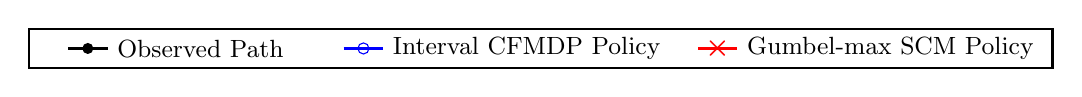
\begin{tikzpicture}[scale=1.0, every node/.style={scale=1.0}]
            \draw[thick, black] (-3, -0.25) rectangle (10, 0.25);
            %
            \draw[black, line width=1pt] (-2.5, 0.0) -- (-2,0.0);
            \fill[black] (-2.25,0.0) circle (2pt); %
            \node[right] at (-2,0.0) {\small Observed Path};
            
            %
            \draw[blue, line width=1pt] (1.0,0.0) -- (1.5,0.0);
            \node[draw=blue, circle, minimum size=4pt, inner sep=0pt] at (1.25,0.0) {}; %
            \node[right] at (1.5,0.0) {\small Interval CFMDP Policy};
            
            %
            \draw[red, line width=1pt] (5.5,0) -- (6,0);
            \node[red] at (5.75,0) {$\boldsymbol{\times}$}; %
            \node[right] at (6,0) {\small Gumbel-max SCM Policy};
        \end{tikzpicture}
    }\\
    %
    \subfigure[\footnotesize Lowest cumulative reward: Interval CFMDP ($312$), Gumbel-max SCM ($312$)]{%
        \resizebox{0.76\columnwidth}{!}{
             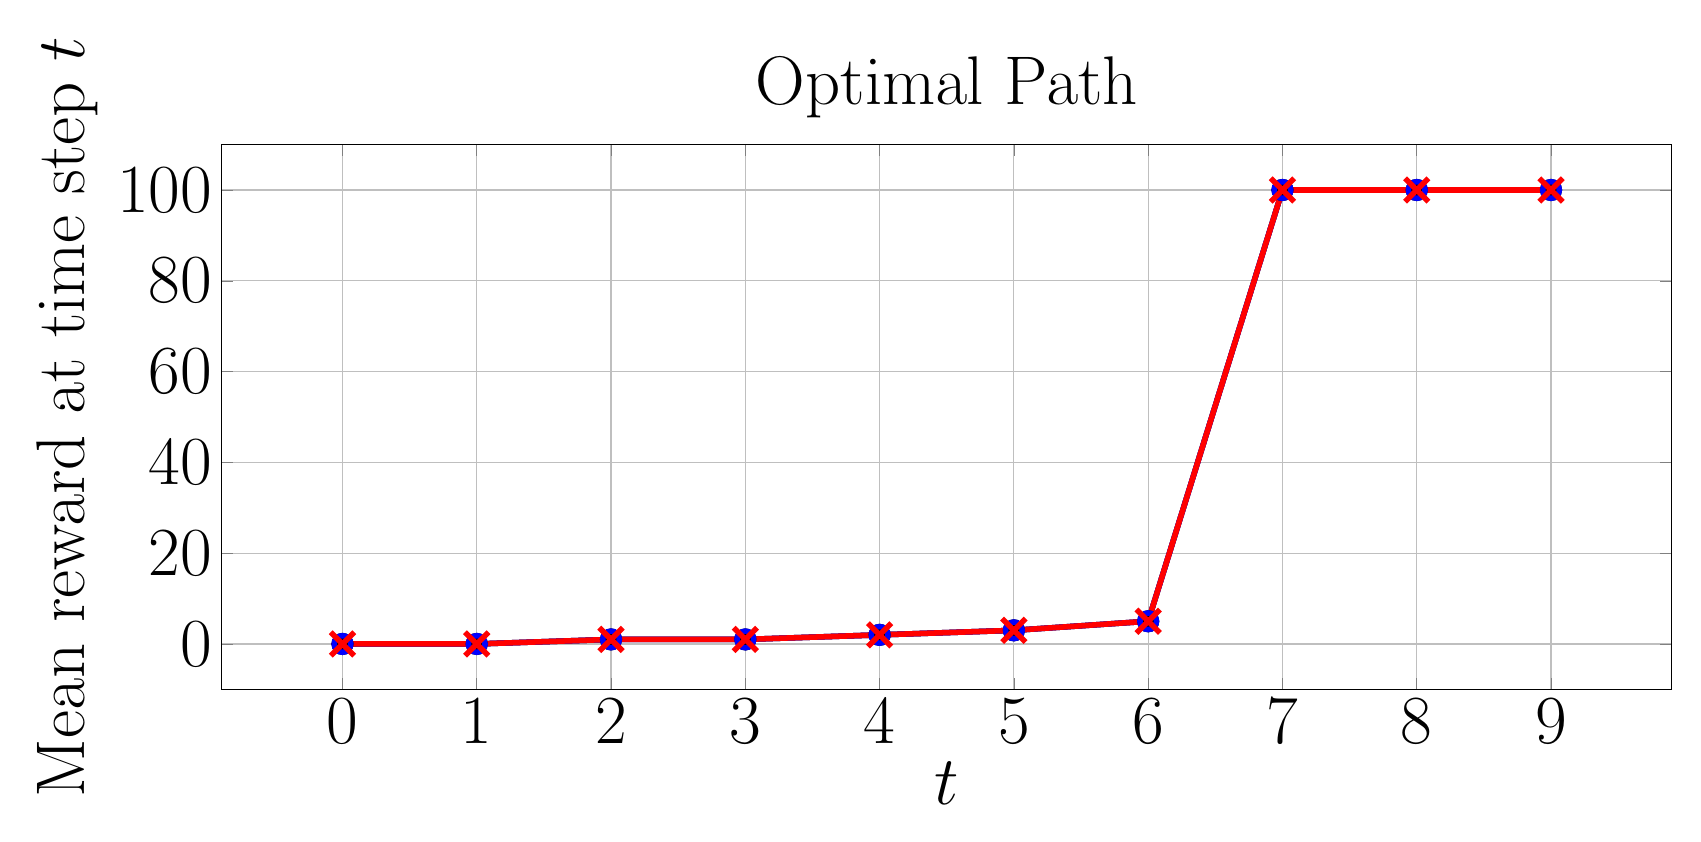
\begin{tikzpicture}
                \begin{axis}[
                    xlabel={$t$},
                    ylabel={Mean reward at time step $t$},
                    title={Optimal Path},
                    grid=both,
                    width=20cm, height=8.5cm,
                    every axis/.style={font=\Huge},
                    %
                ]
                \addplot[
                    color=black, %
                    mark=*, %
                    line width=2pt,
                    mark size=3pt,
                    error bars/.cd,
                    y dir=both, %
                    y explicit, %
                    error bar style={line width=1pt,solid},
                    error mark options={line width=1pt,mark size=4pt,rotate=90}
                ]
                coordinates {
                    (0, 0.0)  +- (0, 0.0)
                    (1, 0.0)  +- (0, 0.0) 
                    (2, 1.0)  +- (0, 0.0) 
                    (3, 1.0)  +- (0, 0.0)
                    (4, 2.0)  +- (0, 0.0)
                    (5, 3.0) +- (0, 0.0)
                    (6, 5.0) +- (0, 0.0)
                    (7, 100.0) +- (0, 0.0)
                    (8, 100.0) +- (0, 0.0)
                    (9, 100.0) +- (0, 0.0)
                };
                %
                \addplot[
                    color=blue, %
                    mark=o, %
                    line width=2pt,
                    mark size=3pt,
                    error bars/.cd,
                    y dir=both, %
                    y explicit, %
                    error bar style={line width=1pt,solid},
                    error mark options={line width=1pt,mark size=4pt,rotate=90}
                ]
                 coordinates {
                    (0, 0.0)  +- (0, 0.0)
                    (1, 0.0)  +- (0, 0.0) 
                    (2, 1.0)  +- (0, 0.0) 
                    (3, 1.0)  +- (0, 0.0)
                    (4, 2.0)  +- (0, 0.0)
                    (5, 3.0) +- (0, 0.0)
                    (6, 5.0) +- (0, 0.0)
                    (7, 100.0) +- (0, 0.0)
                    (8, 100.0) +- (0, 0.0)
                    (9, 100.0) +- (0, 0.0)
                };
                %
                \addplot[
                    color=red, %
                    mark=x, %
                    line width=2pt,
                    mark size=6pt,
                    error bars/.cd,
                    y dir=both, %
                    y explicit, %
                    error bar style={line width=1pt,solid},
                    error mark options={line width=1pt,mark size=4pt,rotate=90}
                ]
                coordinates {
                    (0, 0.0)  +- (0, 0.0)
                    (1, 0.0)  +- (0, 0.0) 
                    (2, 1.0)  +- (0, 0.0) 
                    (3, 1.0)  +- (0, 0.0)
                    (4, 2.0)  +- (0, 0.0)
                    (5, 3.0) +- (0, 0.0)
                    (6, 5.0) +- (0, 0.0)
                    (7, 100.0) +- (0, 0.0)
                    (8, 100.0) +- (0, 0.0)
                    (9, 100.0) +- (0, 0.0)
                };
                \end{axis}
            \end{tikzpicture}
         }
    }
    \hspace{1cm}
    \subfigure[\footnotesize Lowest cumulative reward: Interval CFMDP ($19$), Gumbel-max SCM ($-88$)]{%
         \resizebox{0.76\columnwidth}{!}{
            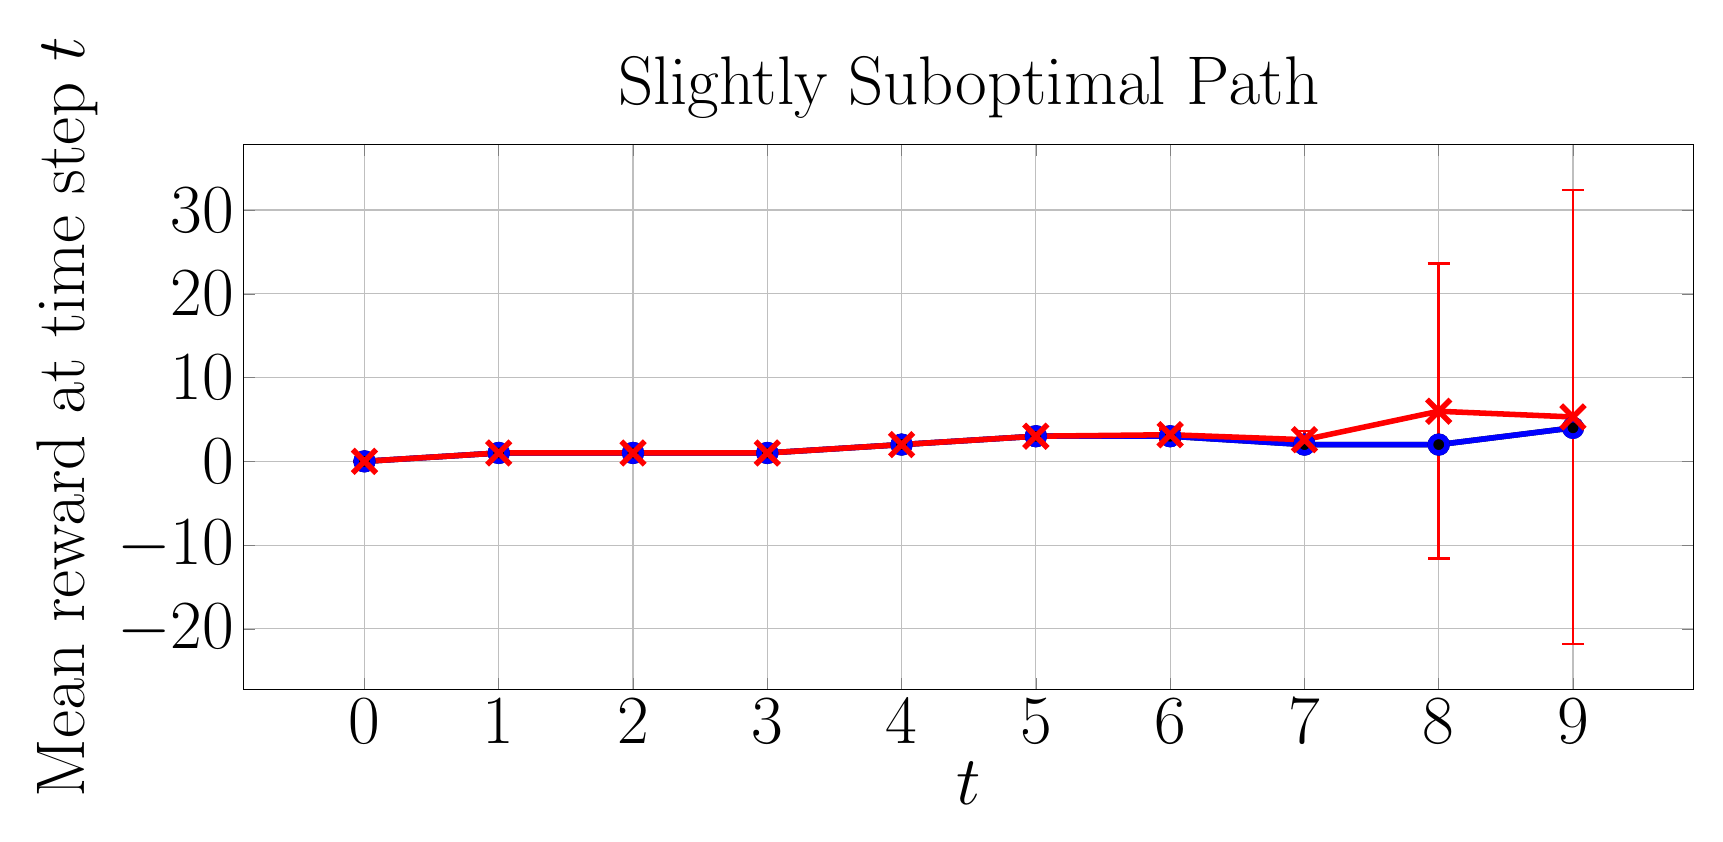
\begin{tikzpicture}
                \begin{axis}[
                    xlabel={$t$},
                    ylabel={Mean reward at time step $t$},
                    title={Slightly Suboptimal Path},
                    grid=both,
                    width=20cm, height=8.5cm,
                    every axis/.style={font=\Huge},
                    %
                ]
                \addplot[
                    color=black, %
                    mark=*, %
                    line width=2pt,
                    mark size=3pt,
                    error bars/.cd,
                    y dir=both, %
                    y explicit, %
                    error bar style={line width=1pt,solid},
                    error mark options={line width=1pt,mark size=4pt,rotate=90}
                ]
              coordinates {
                    (0, 0.0)  +- (0, 0.0)
                    (1, 1.0)  +- (0, 0.0) 
                    (2, 1.0)  +- (0, 0.0) 
                    (3, 1.0)  +- (0, 0.0)
                    (4, 2.0)  +- (0, 0.0)
                    (5, 3.0) +- (0, 0.0)
                    (6, 3.0) +- (0, 0.0)
                    (7, 2.0) +- (0, 0.0)
                    (8, 2.0) +- (0, 0.0)
                    (9, 4.0) +- (0, 0.0)
                };
                %
                \addplot[
                    color=blue, %
                    mark=o, %
                    line width=2pt,
                    mark size=3pt,
                    error bars/.cd,
                    y dir=both, %
                    y explicit, %
                    error bar style={line width=1pt,solid},
                    error mark options={line width=1pt,mark size=4pt,rotate=90}
                ]
              coordinates {
                    (0, 0.0)  +- (0, 0.0)
                    (1, 1.0)  +- (0, 0.0) 
                    (2, 1.0)  +- (0, 0.0) 
                    (3, 1.0)  +- (0, 0.0)
                    (4, 2.0)  +- (0, 0.0)
                    (5, 3.0) +- (0, 0.0)
                    (6, 3.0) +- (0, 0.0)
                    (7, 2.0) +- (0, 0.0)
                    (8, 2.0) +- (0, 0.0)
                    (9, 4.0) +- (0, 0.0)
                };
                %
                \addplot[
                    color=red, %
                    mark=x, %
                    line width=2pt,
                    mark size=6pt,
                    error bars/.cd,
                    y dir=both, %
                    y explicit, %
                    error bar style={line width=1pt,solid},
                    error mark options={line width=1pt,mark size=4pt,rotate=90}
                ]
                coordinates {
                    (0, 0.0)  +- (0, 0.0)
                    (1, 1.0)  +- (0, 0.0) 
                    (2, 1.0)  +- (0, 0.0) 
                    (3, 1.0)  +- (0, 0.0)
                    (4, 2.0)  += (0, 0.0)
                    (5, 3.0)  += (0, 0.0)
                    (6, 3.17847) += (0, 0.62606746) -= (0, 0.62606746)
                    (7, 2.5832885) += (0, 1.04598233) -= (0, 1.04598233)
                    (8, 5.978909) += (0, 17.60137623) -= (0, 17.60137623)
                    (9, 5.297059) += (0, 27.09227512) -= (0, 27.09227512)
                };
                \end{axis}
            \end{tikzpicture}
         }
    }\\[-1.5pt]
    \subfigure[\footnotesize Lowest cumulative reward: Interval CFMDP ($14$), Gumbel-max SCM ($-598$)]{%
         \resizebox{0.76\columnwidth}{!}{
             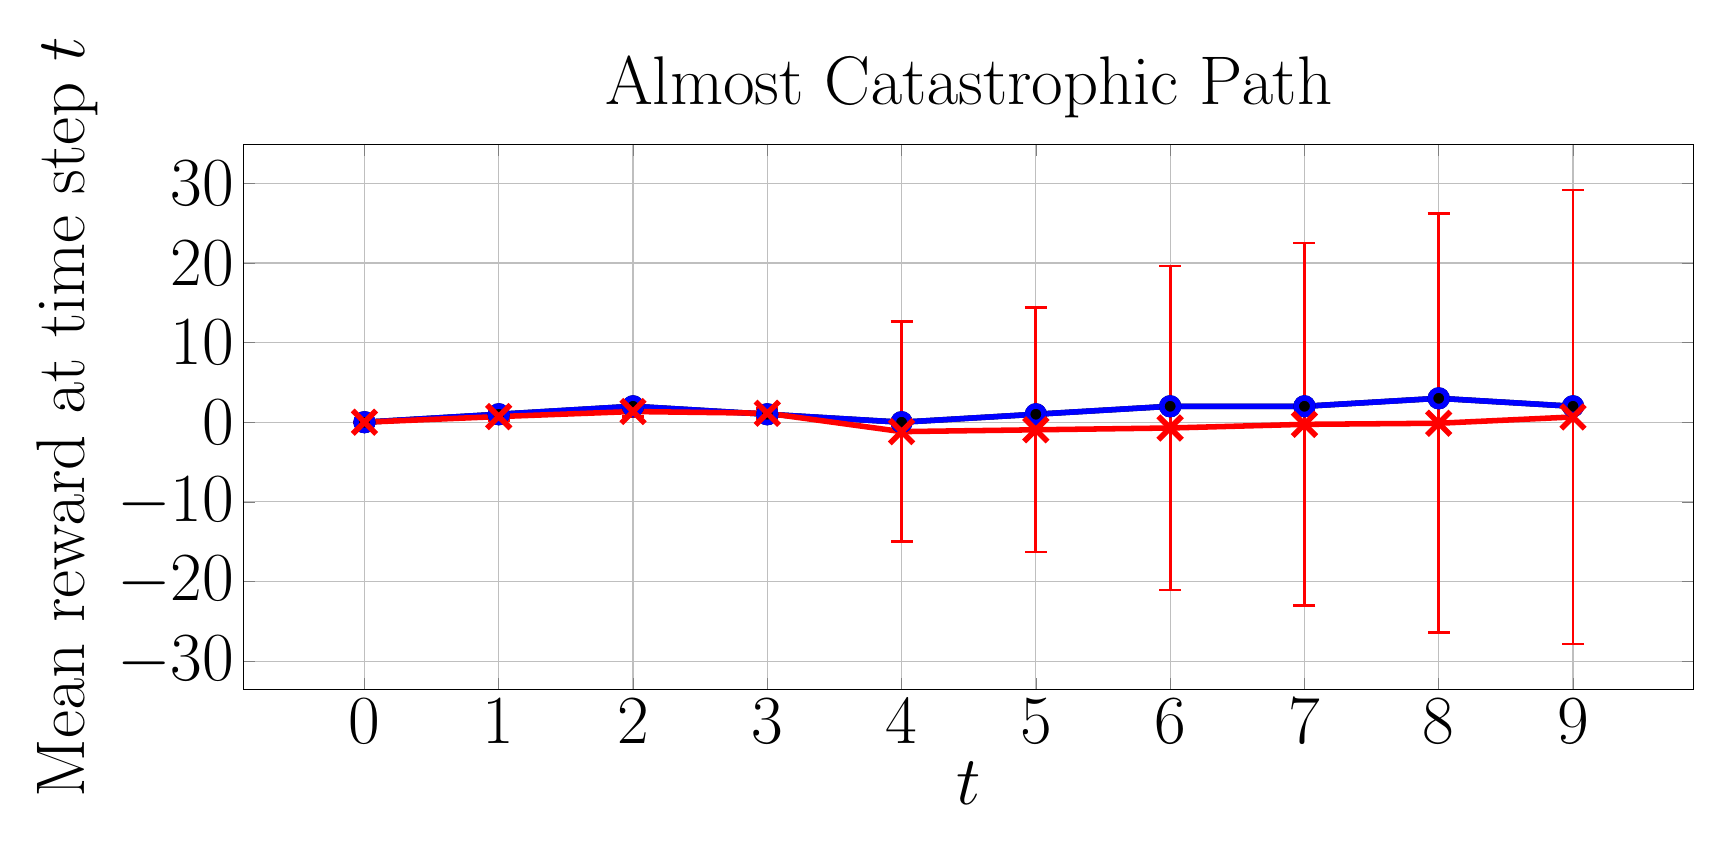
\begin{tikzpicture}
                \begin{axis}[
                    xlabel={$t$},
                    ylabel={Mean reward at time step $t$},
                    title={Almost Catastrophic Path},
                    grid=both,
                    width=20cm, height=8.5cm,
                    every axis/.style={font=\Huge},
                    %
                ]
                \addplot[
                    color=black, %
                    mark=*, %
                    line width=2pt,
                    mark size=3pt,
                    error bars/.cd,
                    y dir=both, %
                    y explicit, %
                    error bar style={line width=1pt,solid},
                    error mark options={line width=1pt,mark size=4pt,rotate=90}
                ]
                coordinates {
                    (0, 0.0)  +- (0, 0.0)
                    (1, 1.0)  +- (0, 0.0) 
                    (2, 2.0)  +- (0, 0.0) 
                    (3, 1.0)  +- (0, 0.0)
                    (4, 0.0)  +- (0, 0.0)
                    (5, 1.0) +- (0, 0.0)
                    (6, 2.0) +- (0, 0.0)
                    (7, 2.0) +- (0, 0.0)
                    (8, 3.0) +- (0, 0.0)
                    (9, 2.0) +- (0, 0.0)
                };
                %
                \addplot[
                    color=blue, %
                    mark=o, %
                    line width=2pt,
                    mark size=3pt,
                    error bars/.cd,
                    y dir=both, %
                    y explicit, %
                    error bar style={line width=1pt,solid},
                    error mark options={line width=1pt,mark size=4pt,rotate=90}
                ]
                coordinates {
                    (0, 0.0)  +- (0, 0.0)
                    (1, 1.0)  +- (0, 0.0) 
                    (2, 2.0)  +- (0, 0.0) 
                    (3, 1.0)  +- (0, 0.0)
                    (4, 0.0)  +- (0, 0.0)
                    (5, 1.0) +- (0, 0.0)
                    (6, 2.0) +- (0, 0.0)
                    (7, 2.0) +- (0, 0.0)
                    (8, 3.0) +- (0, 0.0)
                    (9, 2.0) +- (0, 0.0)
                };
                %
                \addplot[
                    color=red, %
                    mark=x, %
                    line width=2pt,
                    mark size=6pt,
                    error bars/.cd,
                    y dir=both, %
                    y explicit, %
                    error bar style={line width=1pt,solid},
                    error mark options={line width=1pt,mark size=4pt,rotate=90}
                ]
                coordinates {
                    (0, 0.0)  +- (0, 0.0)
                    (1, 0.7065655)  +- (0, 0.4553358) 
                    (2, 1.341673)  +- (0, 0.67091621) 
                    (3, 1.122926)  +- (0, 0.61281824)
                    (4, -1.1821935)  +- (0, 13.82444042)
                    (5, -0.952399)  +- (0, 15.35195457)
                    (6, -0.72672) +- (0, 20.33508414)
                    (7, -0.268983) +- (0, 22.77861454)
                    (8, -0.1310835) +- (0, 26.31013314)
                    (9, 0.65806) +- (0, 28.50670214)
                };
                %
            %
            %
            %
            %
            %
            %
            %
            %
            %
            %
            %
            %
            %
            %
            %
            %
            %
            %
                \end{axis}
            \end{tikzpicture}
         }
    }
    \hspace{1cm}
    \subfigure[\footnotesize Lowest cumulative reward: Interval CFMDP ($-698$), Gumbel-max SCM ($-698$)]{%
         \resizebox{0.76\columnwidth}{!}{
            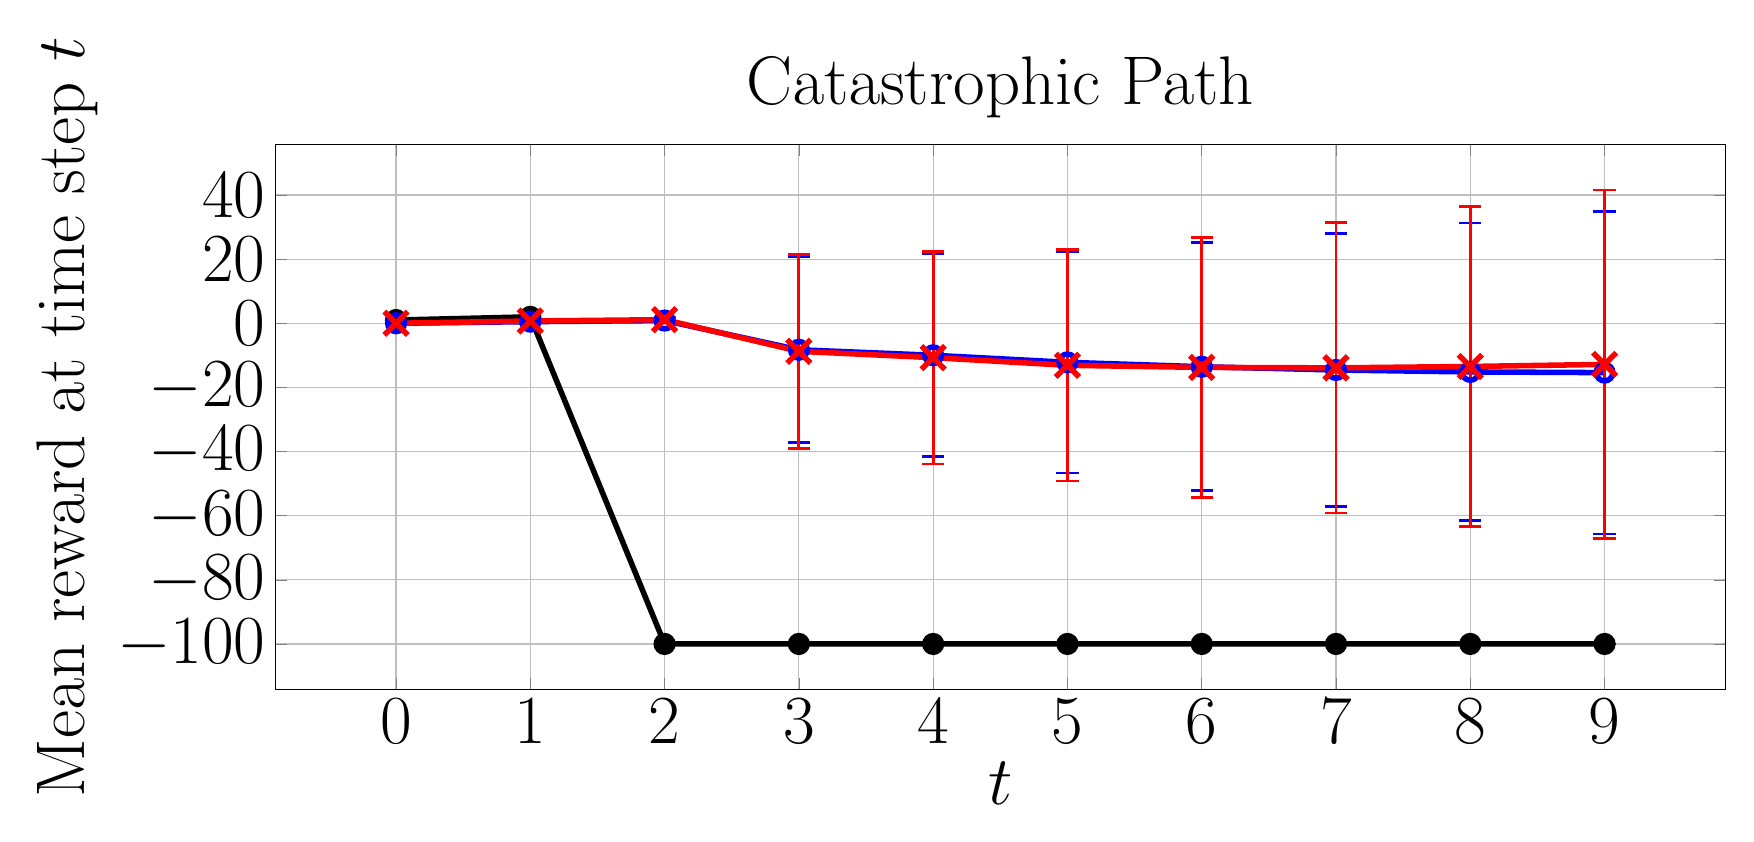
\begin{tikzpicture}
                \begin{axis}[
                    xlabel={$t$},
                    ylabel={Mean reward at time step $t$},
                    title={Catastrophic Path},
                    grid=both,
                    width=20cm, height=8.5cm,
                    every axis/.style={font=\Huge},
                    %
                ]
                \addplot[
                    color=black, %
                    mark=*, %
                    line width=2pt,
                    mark size=3pt,
                    error bars/.cd,
                    y dir=both, %
                    y explicit, %
                    error bar style={line width=1pt,solid},
                    error mark options={line width=1pt,mark size=4pt,rotate=90}
                ]
                coordinates {
                    (0, 1.0)  +- (0, 0.0)
                    (1, 2.0)  +- (0, 0.0) 
                    (2, -100.0)  +- (0, 0.0) 
                    (3, -100.0)  +- (0, 0.0)
                    (4, -100.0)  +- (0, 0.0)
                    (5, -100.0) +- (0, 0.0)
                    (6, -100.0) +- (0, 0.0)
                    (7, -100.0) +- (0, 0.0)
                    (8, -100.0) +- (0, 0.0)
                    (9, -100.0) +- (0, 0.0)
                };
                %
                \addplot[
                    color=blue, %
                    mark=o, %
                    line width=2pt,
                    mark size=3pt,
                    error bars/.cd,
                    y dir=both, %
                    y explicit, %
                    error bar style={line width=1pt,solid},
                    error mark options={line width=1pt,mark size=4pt,rotate=90}
                ]
                coordinates {
                    (0, 0.0)  +- (0, 0.0)
                    (1, 0.504814)  +- (0, 0.49997682) 
                    (2, 0.8439835)  +- (0, 0.76831917) 
                    (3, -8.2709165)  +- (0, 28.93656754)
                    (4, -9.981082)  +- (0, 31.66825363)
                    (5, -12.1776325) +- (0, 34.53463233)
                    (6, -13.556076) +- (0, 38.62845372)
                    (7, -14.574418) +- (0, 42.49603359)
                    (8, -15.1757075) +- (0, 46.41913968)
                    (9, -15.3900395) +- (0, 50.33563368)
                };
                %
                \addplot[
                    color=red, %
                    mark=x, %
                    line width=2pt,
                    mark size=6pt,
                    error bars/.cd,
                    y dir=both, %
                    y explicit, %
                    error bar style={line width=1pt,solid},
                    error mark options={line width=1pt,mark size=4pt,rotate=90}
                ]
                coordinates {
                    (0, 0.0)  +- (0, 0.0)
                    (1, 0.701873)  +- (0, 0.45743556) 
                    (2, 1.1227805)  +- (0, 0.73433129) 
                    (3, -8.7503255)  +- (0, 30.30257976)
                    (4, -10.722092)  +- (0, 33.17618589)
                    (5, -13.10721)  +- (0, 36.0648089)
                    (6, -13.7631645) +- (0, 40.56553451)
                    (7, -13.909043) +- (0, 45.23829402)
                    (8, -13.472517) +- (0, 49.96270296)
                    (9, -12.8278835) +- (0, 54.38618735)
                };
                %
            %
            %
            %
            %
            %
            %
            %
            %
            %
            %
            %
            %
            %
            %
            %
            %
            %
            %
                \end{axis}
            \end{tikzpicture}
         }
    }
    \caption{Average instant reward of CF paths induced by policies on GridWorld $p=0.4$.}
    \label{fig: reward p=0.4}
\end{figure*}

\subsection{Experimental Setup}
To compare policy performance, we measure the average rewards of counterfactual paths induced by our policy and the Gumbel-max policy by uniformly sampling $200$ counterfactual MDPs from the ICFMDP and generating $10,000$ counterfactual paths over each sampled CFMDP. \jl{Since the interval CFMDP depends on the observed path, we select $4$  paths of varying optimality to evaluate how the observed path impacts the performance of both policies: an optimal path, a slightly suboptimal path that could reach the optimal reward with a few changes, a catastrophic path that enters a catastrophic, terminal state with low reward, and an almost catastrophic path that was close to entering a catastrophic state.} When measuring the average probability bound widths and execution time needed to generate the ICFMDPs, we averaged over $20$ randomly generated observed paths
\footnote{Further training details are provided in Appendix \ref{app: training details}, and the code is provided at \href{https://github.com/ddv-lab/robust-cf-inference-in-MDPs}{https://github.com/ddv-lab/robust-cf-inference-in-MDPs}
%
%
.}.

\subsection{GridWorld}
\jl{The GridWorld MDP is a $4 \times 4$ grid where an agent must navigate from the top-left corner to the goal state in the bottom-right corner, avoiding a dangerous terminal state in the centre. At each time step, the agent can move up, down, left, or right, but there is a small probability (controlled by hyper-parameter $p$) of moving in an unintended direction. As the agent nears the goal, the reward for each state increases, culminating in a reward of $+100$ for reaching the goal. Entering the dangerous state results in a penalty of $-100$. We use two versions of GridWorld: a less stochastic version with $p=0.9$ (i.e., $90$\% chance of moving in the chosen direction) and a more stochastic version with $p=0.4$.}

\paragraph{GridWorld ($p=0.9$)}
When $p=0.9$, the counterfactual probability bounds are typically narrow (see Table \ref{tab:nonzero_probs} for average measurements). Consequently, as shown in Figure \ref{fig: reward p=0.9}, both policies are nearly identical and perform similarly well across the optimal, slightly suboptimal, and catastrophic paths.
%
However, for the almost catastrophic path, the interval CFMDP path is more conservative and follows the observed path more closely (as this is where the probability bounds are narrowest), which typically requires one additional step to reach the goal state than the Gumbel-max SCM policy.
%

\paragraph{GridWorld ($p=0.4$)}
\jl{When $p=0.4$, the GridWorld environment becomes more uncertain, increasing the risk of entering the dangerous state even if correct actions are chosen. Thus, as shown in Figure \ref{fig: reward p=0.4}, the interval CFMDP policy adopts a more conservative approach, avoiding deviation from the observed policy if it cannot guarantee higher counterfactual rewards (see the slightly suboptimal and almost catastrophic paths), whereas the Gumbel-max SCM is inconsistent: it can yield higher rewards, but also much lower rewards, reflected in the wide error bars.} For the catastrophic path, both policies must deviate from the observed path to achieve a higher reward and, in this case, perform similarly.
%
%
%
%
\subsection{Sepsis}
The Sepsis MDP \citep{oberst2019counterfactual} simulates trajectories of Sepsis patients. Each state consists of four vital signs (heart rate, blood pressure, oxygen concentration, and glucose levels), categorised as low, normal, or high.
and three treatments that can be toggled on/off at each time step (8 actions in total). Unlike \citet{oberst2019counterfactual}, we scale rewards based on the number of out-of-range vital signs, between $-1000$ (patient dies) and $1000$ (patient discharged). \jl{Like the GridWorld $p=0.4$ experiment, the Sepsis MDP is highly uncertain, as many states are equally likely to lead to optimal and poor outcomes. Thus, as shown in Figure \ref{fig: reward sepsis}, both policies follow the observed optimal and almost catastrophic paths to guarantee rewards are no worse than the observation.} However, improving the catastrophic path requires deviating from the observation. Here, the Gumbel-max SCM policy, on average, performs better than the interval CFMDP policy. But, since both policies have lower bounds clipped at $-1000$, neither policy reliably improves over the observation. In contrast, for the slightly suboptimal path, the interval CFMDP policy performs significantly better, shown by its higher lower bounds. 
Moreover, in these two cases, the worst-case counterfactual path generated by the interval CFMDP policy is better than that of the Gumbel-max SCM policy,
indicating its greater robustness.
%
\begin{figure*}
    \centering
     \resizebox{0.6\textwidth}{!}{
        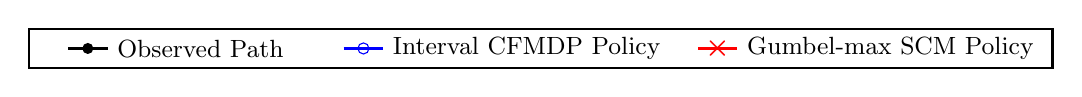
\begin{tikzpicture}[scale=1.0, every node/.style={scale=1.0}]
            \draw[thick, black] (-3, -0.25) rectangle (10, 0.25);
            %
            \draw[black, line width=1pt] (-2.5, 0.0) -- (-2,0.0);
            \fill[black] (-2.25,0.0) circle (2pt); %
            \node[right] at (-2,0.0) {\small Observed Path};
            
            %
            \draw[blue, line width=1pt] (1.0,0.0) -- (1.5,0.0);
            \node[draw=blue, circle, minimum size=4pt, inner sep=0pt] at (1.25,0.0) {}; %
            \node[right] at (1.5,0.0) {\small Interval CFMDP Policy};
            
            %
            \draw[red, line width=1pt] (5.5,0) -- (6,0);
            \node[red] at (5.75,0) {$\boldsymbol{\times}$}; %
            \node[right] at (6,0) {\small Gumbel-max SCM Policy};
        \end{tikzpicture}
    }\\
    \subfigure[\footnotesize Lowest cumulative reward: Interval CFMDP ($8000$), Gumbel-max SCM ($8000$)]{%
         \resizebox{0.76\columnwidth}{!}{
             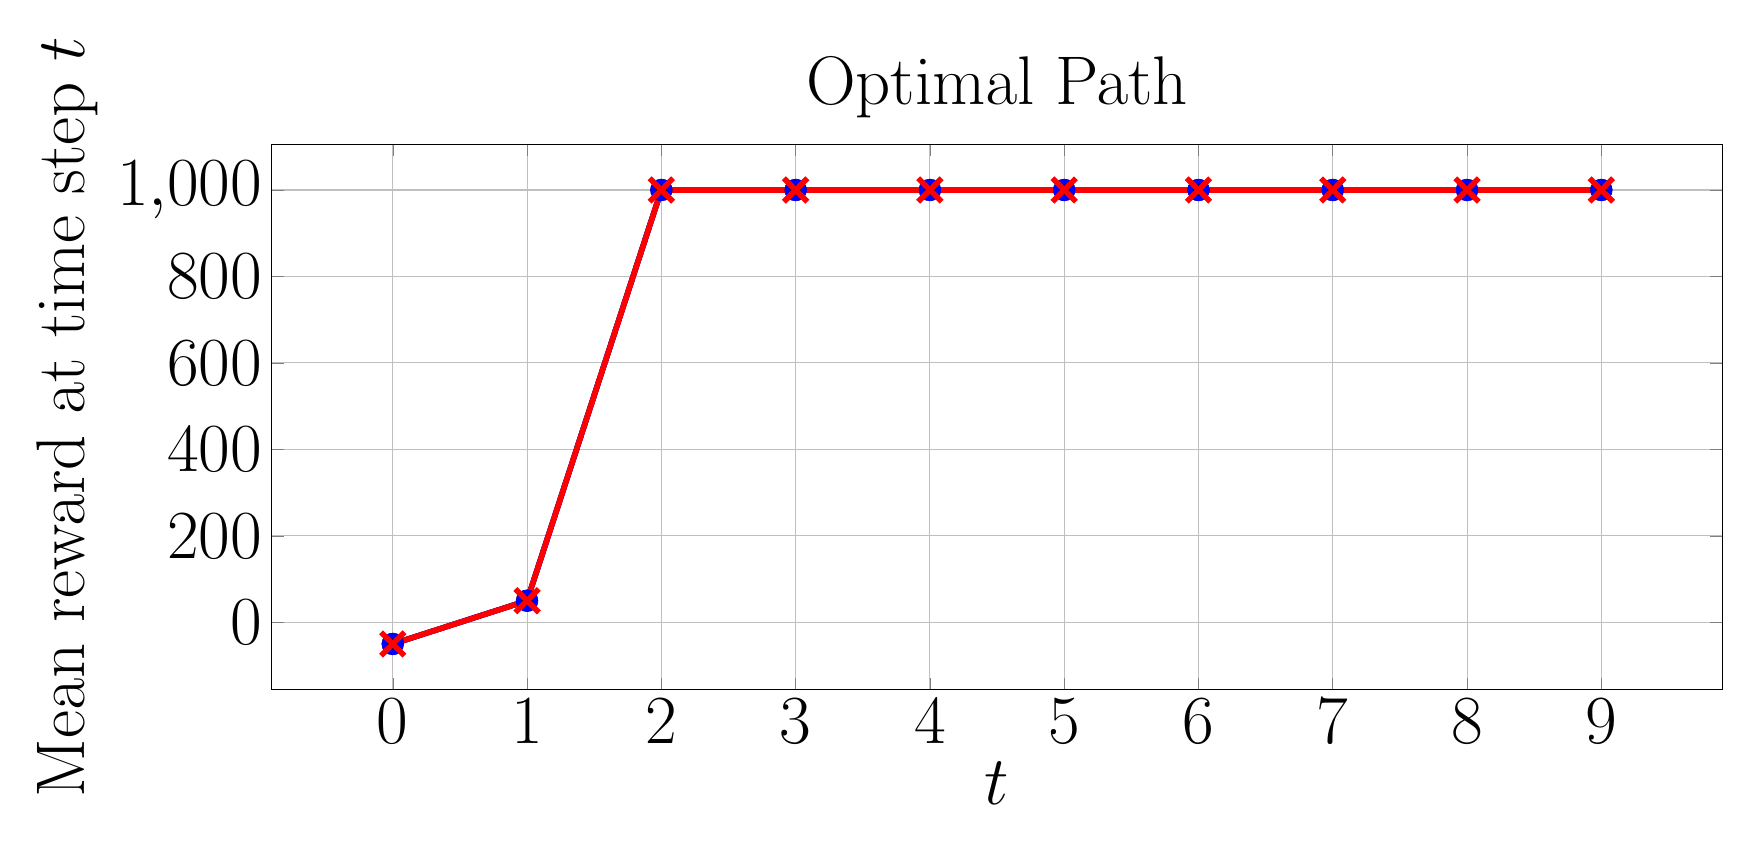
\begin{tikzpicture}
                \begin{axis}[
                    xlabel={$t$},
                    ylabel={Mean reward at time step $t$},
                    title={Optimal Path},
                    grid=both,
                    width=20cm, height=8.5cm,
                    every axis/.style={font=\Huge},
                    %
                ]
                \addplot[
                    color=black, %
                    mark=*, %
                    line width=2pt,
                    mark size=3pt,
                ]
                coordinates {
                    (0, -50.0)
                    (1, 50.0)
                    (2, 1000.0)
                    (3, 1000.0)
                    (4, 1000.0)
                    (5, 1000.0)
                    (6, 1000.0)
                    (7, 1000.0)
                    (8, 1000.0)
                    (9, 1000.0)
                };
                %
                \addplot[
                    color=blue, %
                    mark=o, %
                    line width=2pt,
                    mark size=3pt,
                    error bars/.cd,
                    y dir=both, %
                    y explicit, %
                    error bar style={line width=1pt,solid},
                    error mark options={line width=1pt,mark size=4pt,rotate=90}
                ]
                coordinates {
                    (0, -50.0)  +- (0, 0.0)
                    (1, 50.0)  +- (0, 0.0) 
                    (2, 1000.0)  +- (0, 0.0) 
                    (3, 1000.0)  +- (0, 0.0)
                    (4, 1000.0)  +- (0, 0.0)
                    (5, 1000.0) +- (0, 0.0)
                    (6, 1000.0) +- (0, 0.0)
                    (7, 1000.0) +- (0, 0.0)
                    (8, 1000.0) +- (0, 0.0)
                    (9, 1000.0) +- (0, 0.0)
                };
                %
                \addplot[
                    color=red, %
                    mark=x, %
                    line width=2pt,
                    mark size=6pt,
                    error bars/.cd,
                    y dir=both, %
                    y explicit, %
                    error bar style={line width=1pt,solid},
                    error mark options={line width=1pt,mark size=4pt,rotate=90}
                ]
                coordinates {
                    (0, -50.0)  +- (0, 0.0)
                    (1, 50.0)  +- (0, 0.0) 
                    (2, 1000.0)  +- (0, 0.0) 
                    (3, 1000.0)  +- (0, 0.0)
                    (4, 1000.0)  +- (0, 0.0)
                    (5, 1000.0) +- (0, 0.0)
                    (6, 1000.0) +- (0, 0.0)
                    (7, 1000.0) +- (0, 0.0)
                    (8, 1000.0) +- (0, 0.0)
                    (9, 1000.0) +- (0, 0.0)
                };
                %
                \end{axis}
            \end{tikzpicture}
         }
    }
    \hspace{1cm}
    \subfigure[\footnotesize Lowest cumulative reward: Interval CFMDP ($-5980$), Gumbel-max SCM ($-8000$)]{%
         \resizebox{0.76\columnwidth}{!}{
            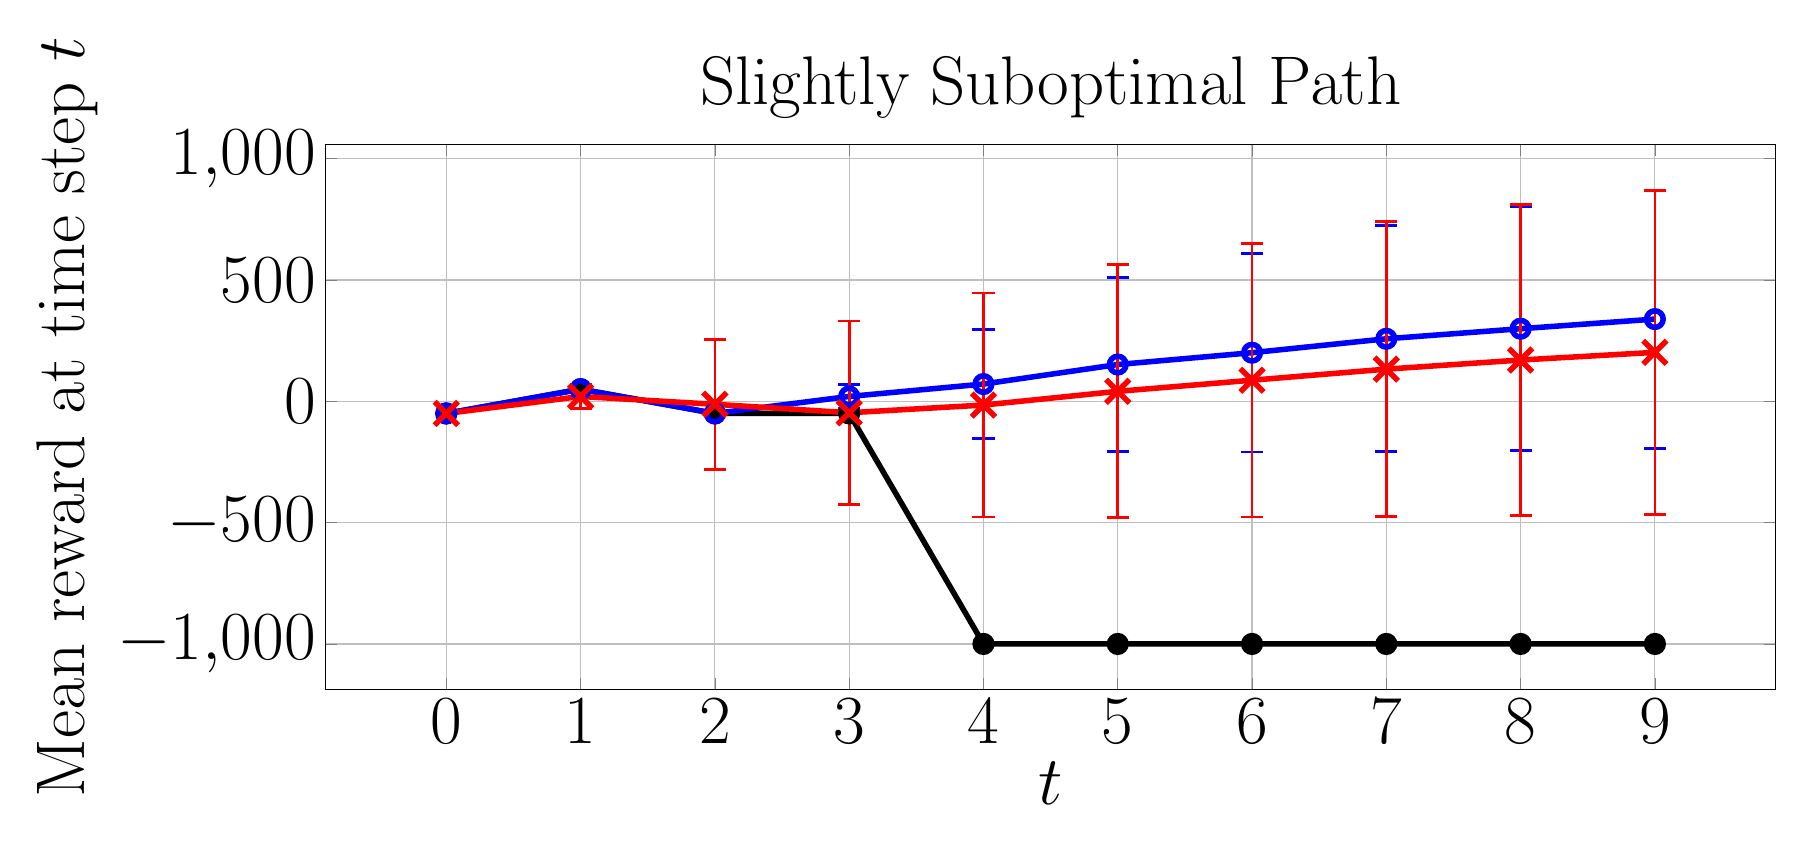
\begin{tikzpicture}
                \begin{axis}[
                    xlabel={$t$},
                    ylabel={Mean reward at time step $t$},
                    title={Slightly Suboptimal Path},
                    grid=both,
                    width=20cm, height=8.5cm,
                    every axis/.style={font=\Huge},
                    %
                ]
               \addplot[
                    color=black, %
                    mark=*, %
                    line width=2pt,
                    mark size=3pt,
                ]
                coordinates {
                    (0, -50.0)
                    (1, 50.0)
                    (2, -50.0)
                    (3, -50.0)
                    (4, -1000.0)
                    (5, -1000.0)
                    (6, -1000.0)
                    (7, -1000.0)
                    (8, -1000.0)
                    (9, -1000.0)
                };
                %
                \addplot[
                    color=blue, %
                    mark=o, %
                    line width=2pt,
                    mark size=3pt,
                    error bars/.cd,
                    y dir=both, %
                    y explicit, %
                    error bar style={line width=1pt,solid},
                    error mark options={line width=1pt,mark size=4pt,rotate=90}
                ]
                coordinates {
                    (0, -50.0)  +- (0, 0.0)
                    (1, 50.0)  +- (0, 0.0) 
                    (2, -50.0)  +- (0, 0.0) 
                    (3, 20.0631)  +- (0, 49.97539413)
                    (4, 71.206585)  +- (0, 226.02033693)
                    (5, 151.60797) +- (0, 359.23292559)
                    (6, 200.40593) +- (0, 408.86185176)
                    (7, 257.77948) +- (0, 466.10372804)
                    (8, 299.237465) +- (0, 501.82579506)
                    (9, 338.9129) +- (0, 532.06124996)
                };
                %
                \addplot[
                    color=red, %
                    mark=x, %
                    line width=2pt,
                    mark size=6pt,
                    error bars/.cd,
                    y dir=both, %
                    y explicit, %
                    error bar style={line width=1pt,solid},
                    error mark options={line width=1pt,mark size=4pt,rotate=90}
                ]
                coordinates {
                    (0, -50.0)  +- (0, 0.0)
                    (1, 20.00736)  +- (0, 49.99786741) 
                    (2, -12.282865)  +- (0, 267.598755) 
                    (3, -47.125995)  +- (0, 378.41755832)
                    (4, -15.381965)  +- (0, 461.77616558)
                    (5, 41.15459) +- (0, 521.53189262)
                    (6, 87.01595) +- (0, 564.22243126 )
                    (7, 132.62376) +- (0, 607.31338037)
                    (8, 170.168145) +- (0, 641.48013693)
                    (9, 201.813135) +- (0, 667.29441777)
                };
                %
                %
                %
                %
                %
                %
                %
                %
                %
                %
                %
                %
                %
                %
                %
                %
                %
                %
                %
                \end{axis}
            \end{tikzpicture}
         }
    }\\[-1.5pt]
    \subfigure[\footnotesize Lowest cumulative reward: Interval CFMDP ($100$), Gumbel-max SCM ($100$)]{%
         \resizebox{0.76\columnwidth}{!}{
             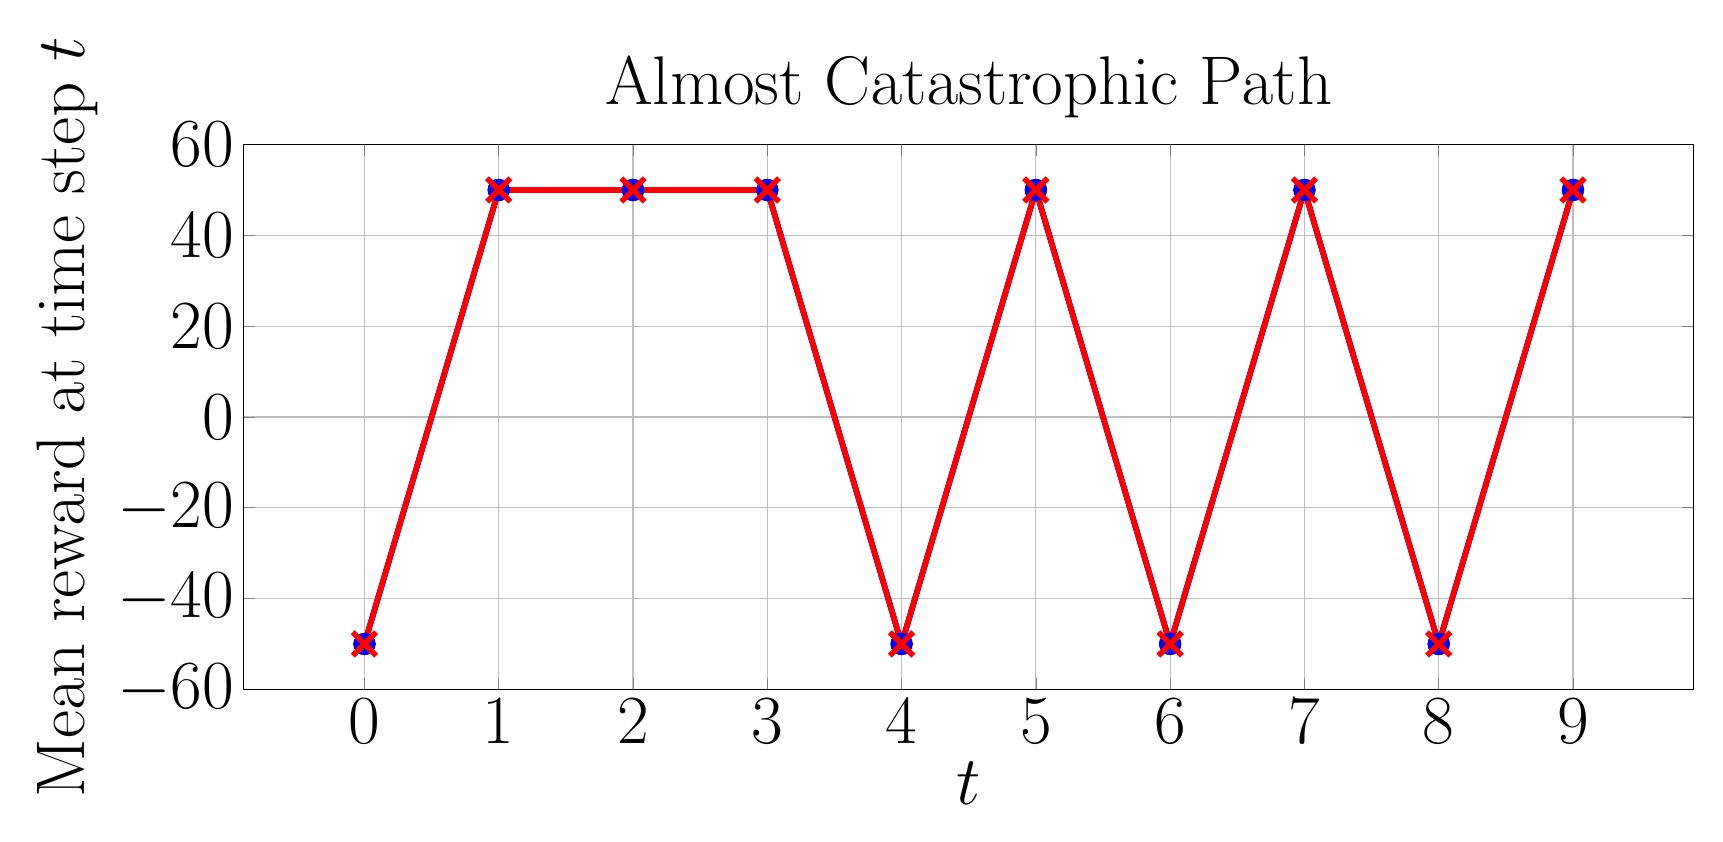
\begin{tikzpicture}
                \begin{axis}[
                    xlabel={$t$},
                    ylabel={Mean reward at time step $t$},
                    title={Almost Catastrophic Path},
                    grid=both,
                    every axis/.style={font=\Huge},
                    width=20cm, height=8.5cm,
                    %
                ]
               \addplot[
                    color=black, %
                    mark=*, %
                    line width=2pt,
                    mark size=3pt,
                ]
                coordinates {
                    (0, -50.0)
                    (1, 50.0)
                    (2, 50.0)
                    (3, 50.0)
                    (4, -50.0)
                    (5, 50.0)
                    (6, -50.0)
                    (7, 50.0)
                    (8, -50.0)
                    (9, 50.0)
                };
                %
                %
                \addplot[
                    color=blue, %
                    mark=o, %
                    line width=2pt,
                    mark size=3pt,
                    error bars/.cd,
                    y dir=both, %
                    y explicit, %
                    error bar style={line width=1pt,solid},
                    error mark options={line width=1pt,mark size=4pt,rotate=90}
                ]
                coordinates {
                    (0, -50.0)  +- (0, 0.0)
                    (1, 50.0)  +- (0, 0.0) 
                    (2, 50.0)  +- (0, 0.0) 
                    (3, 50.0)  +- (0, 0.0)
                    (4, -50.0)  +- (0, 0.0)
                    (5, 50.0) +- (0, 0.0)
                    (6, -50.0) +- (0, 0.0)
                    (7, 50.0) +- (0, 0.0)
                    (8, -50.0) +- (0, 0.0)
                    (9, 50.0) +- (0, 0.0)
                };
                %
                \addplot[
                    color=red, %
                    mark=x, %
                    line width=2pt,
                    mark size=6pt,
                    error bars/.cd,
                    y dir=both, %
                    y explicit, %
                    error bar style={line width=1pt,solid},
                    error mark options={line width=1pt,mark size=4pt,rotate=90}
                ]
                coordinates {
                    (0, -50.0)  +- (0, 0.0)
                    (1, 50.0)  +- (0, 0.0) 
                    (2, 50.0)  +- (0, 0.0) 
                    (3, 50.0)  +- (0, 0.0)
                    (4, -50.0)  +- (0, 0.0)
                    (5, 50.0) +- (0, 0.0)
                    (6, -50.0) +- (0, 0.0)
                    (7, 50.0) +- (0, 0.0)
                    (8, -50.0) +- (0, 0.0)
                    (9, 50.0) +- (0, 0.0)
                };
                %
                %
                %
                %
                %
                %
                %
                %
                %
                %
                %
                %
                %
                %
                %
                %
                %
                %
                %
                \end{axis}
            \end{tikzpicture}
         }
    }
    \hspace{1cm}
    \subfigure[\footnotesize Lowest cumulative reward: Interval CFMDP ($-7150$), Gumbel-max SCM ($-9050$)]{%
         \resizebox{0.76\columnwidth}{!}{
            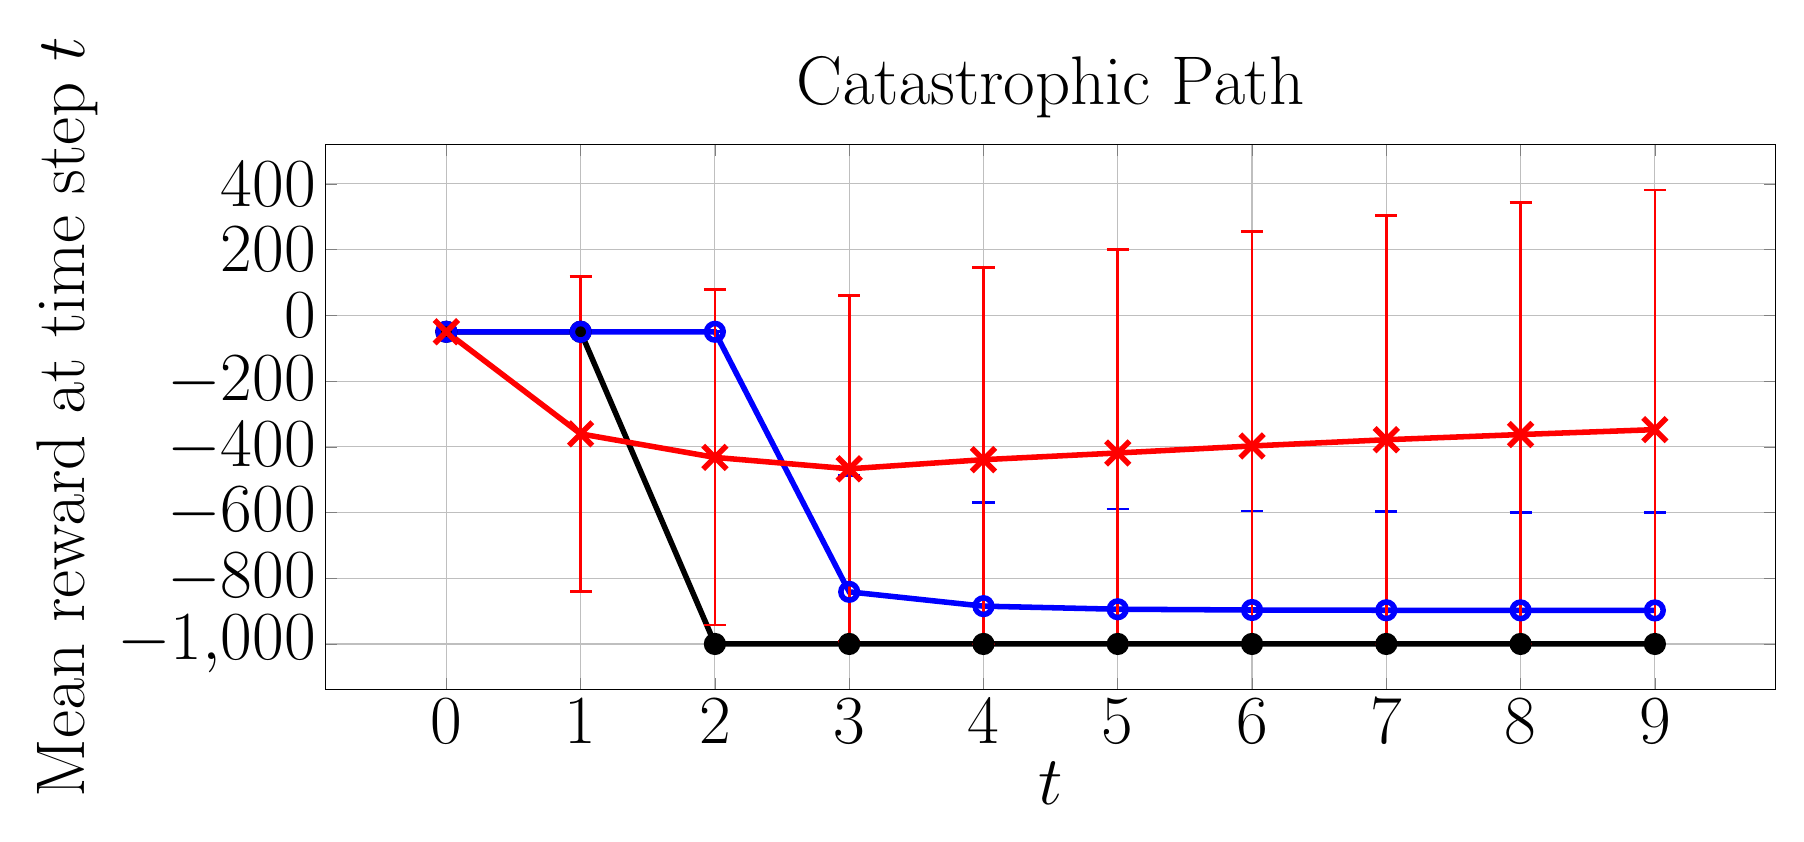
\begin{tikzpicture}
                \begin{axis}[
                    xlabel={$t$},
                    ylabel={Mean reward at time step $t$},
                    title={Catastrophic Path},
                    grid=both,
                    width=20cm, height=8.5cm,
                    every axis/.style={font=\Huge},
                    %
                ]
               \addplot[
                    color=black, %
                    mark=*, %
                    line width=2pt,
                    mark size=3pt,
                ]
                coordinates {
                    (0, -50.0)
                    (1, -50.0)
                    (2, -1000.0)
                    (3, -1000.0)
                    (4, -1000.0)
                    (5, -1000.0)
                    (6, -1000.0)
                    (7, -1000.0)
                    (8, -1000.0)
                    (9, -1000.0)
                };
                %
                %
                \addplot[
                    color=blue, %
                    mark=o, %
                    line width=2pt,
                    mark size=3pt,
                    error bars/.cd,
                    y dir=both, %
                    y explicit, %
                    error bar style={line width=1pt,solid},
                    error mark options={line width=1pt,mark size=4pt,rotate=90}
                ]
                coordinates {
                    (0, -50.0)  +- (0, 0.0)
                    (1, -50.0)  +- (0, 0.0) 
                    (2, -50.0)  +- (0, 0.0) 
                    (3, -841.440725)  += (0, 354.24605512) -= (0, 158.559275)
                    (4, -884.98225)  += (0, 315.37519669) -= (0, 115.01775)
                    (5, -894.330425) += (0, 304.88572805) -= (0, 105.669575)
                    (6, -896.696175) += (0, 301.19954514) -= (0, 103.303825)
                    (7, -897.4635) += (0, 299.61791279) -= (0, 102.5365)
                    (8, -897.77595) += (0, 298.80392585) -= (0, 102.22405)
                    (9, -897.942975) += (0, 298.32920557) -= (0, 102.057025)
                };
                %
                \addplot[
                    color=red, %
                    mark=x, %
                    line width=2pt,
                    mark size=6pt,
                    error bars/.cd,
                    y dir=both, %
                    y explicit, %
                    error bar style={line width=1pt,solid},
                    error mark options={line width=1pt,mark size=4pt,rotate=90}
                ]
            coordinates {
                    (0, -50.0)  +- (0, 0.0)
                    (1, -360.675265)  +- (0, 479.39812699) 
                    (2, -432.27629)  +- (0, 510.38620897) 
                    (3, -467.029545)  += (0, 526.36009628) -= (0, 526.36009628)
                    (4, -439.17429)  += (0, 583.96638919) -= (0, 560.82571)
                    (5, -418.82704) += (0, 618.43027478) -= (0, 581.17296)
                    (6, -397.464895) += (0, 652.67322574) -= (0, 602.535105)
                    (7, -378.49052) += (0, 682.85407033) -= (0, 621.50948)
                    (8, -362.654195) += (0, 707.01412023) -= (0, 637.345805)
                    (9, -347.737935) += (0, 729.29076479) -= (0, 652.262065)
                };
                %
                %
                %
                %
                %
                %
                %
                %
                %
                %
                %
                %
                %
                %
                %
                %
                %
                %
                %
                \end{axis}
            \end{tikzpicture}
         }
    }
    \caption{Average instant reward of CF paths induced by policies on Sepsis.}
    \label{fig: reward sepsis}
\end{figure*}

%
%
%
\subsection{Interval CFMDP Bounds}
%
%
Table \ref{tab:nonzero_probs} presents the mean counterfactual probability bound widths (excluding transitions where the upper bound is $0$) for each MDP, averaged over 20 observed paths. We compare the bounds under counterfactual stability (CS) and monotonicity (M) assumptions, CS alone, and no assumptions. This shows that the assumptions marginally reduce the bound widths, indicating the assumptions tighten the bounds without excluding too many causal models, as intended.
\renewcommand{\arraystretch}{1}

\begin{table}
\centering
\caption{Mean width of counterfactual probability bounds}
\resizebox{0.8\columnwidth}{!}{%
\begin{tabular}{|c|c|c|c|}
\hline
\multirow{2}{*}{\textbf{Environment}} & \multicolumn{3}{c|}{\textbf{Assumptions}} \\ \cline{2-4}
 & \textbf{CS + M} & \textbf{CS} & \textbf{None\tablefootnote{\jl{Equivalent to \citet{li2024probabilities}'s bounds (see Section \ref{sec: equivalence with Li}).}}} \\ \hline
\textbf{GridWorld} ($p=0.9$) & 0.0817 & 0.0977 & 0.100 \\ \hline
\textbf{GridWorld} ($p=0.4$) & 0.552  & 0.638  & 0.646 \\ \hline
\textbf{Sepsis} & 0.138 & 0.140 & 0.140 \\ \hline
\end{tabular}
}
\label{tab:nonzero_probs}
\end{table}


\subsection{Execution Times}
Table \ref{tab: times} compares the average time needed to generate the interval CFMDP vs.\ the Gumbel-max SCM CFMDP for 20 observations.
The GridWorld algorithms were run single-threaded, while the Sepsis experiments were run in parallel.
Generating the interval CFMDP is significantly faster as it uses exact analytical bounds, whereas the Gumbel-max CFMDP requires sampling from the Gumbel distribution to estimate counterfactual transition probabilities. \jl{Since constructing the counterfactual MDP models is the main bottleneck in both approaches, ours is more efficient overall and suitable for larger MDPs.}
\begin{table}
\centering
\caption{Mean execution time to generate CFMDPs}
\resizebox{0.99\columnwidth}{!}{%
\begin{tabular}{|c|c|c|}
\hline
\multirow{2}{*}{\textbf{Environment}} & \multicolumn{2}{c|}{\textbf{Mean Execution Time (s)}} \\ \cline{2-3} 
                                      & \textbf{Interval CFMDP} & \textbf{Gumbel-max CFMDP} \\ \hline
\textbf{GridWorld ($p=0.9$) }                  & 0.261                   & 56.1                      \\ \hline
\textbf{GridWorld ($p=0.4$)  }                 & 0.336                   & 54.5                      \\ \hline
\textbf{Sepsis}                                 & 688                     & 2940                      \\ \hline
\end{tabular}%
}
\label{tab: times}
\end{table}

% -> Experiment의 subsection으로 insert

%\section{Result}
%\section{Result} \label{sec:result}

\subsection{Setup}

In this section, we evaluate VB-Com across the following perspectives:
\begin{itemize}
    \item Under what conditions does VB-Com demonstrate superior performance compared to using a single-policy approach?
    \item How does VB-Com outperforms baseline methods in those scenarios?
    \item How well does the proposed return estimator contribute to the composition system?
\end{itemize}

\begin{figure}[h]
\centering{\includegraphics[width=0.5\textwidth]{figures/noise.png}}
\caption{We present four types of perception noises and implement them on heightmaps during evaluation: gaussian noise, \textcolor{red}{forward shifting noise}, \textcolor{green}{lateral shifting noise} and \textcolor{blue}{floating noise}.}
\label{noise}
\end{figure}

\subsubsection{Evaluation Noise}
To simulate situations where the robot encounters perception outliers not present in the simulation, we introduce a quantitative curriculum noise designed to mimic varying levels of perception deficiency. As shown in Fig. \ref{noise}, we focus on four types of noise: (1) \textbf{Gaussian noise}: noise points sampled from a Gaussian distribution, to the original heightmap. The noise level is scaled from 0.0 to 1.0, where the training noise level corresponds to a 0.1 noise level in this scenario. (2) \textbf{Shifting noise}: replacing points in the original heightmap with noise sampled from a Gaussian distribution. The range of replacement points is controlled by the noise level, where a $100\%$ noise level results in a fully noisy heightmap. The shifting direction can either be along the heading direction (red box) or sideways (green box). (3) \textbf{Floating noise}: The heightmap is displaced vertically, either upwards or downwards, the floating noise simulates variations in terrain height. (blue box).

\begin{table}[!ht]
\caption{Terrain Size Scales (m)}
\label{tab:terrains}
\begin{center}
\renewcommand\arraystretch{1.25}
\begin{tabular}{lcccc}
\toprule[1.0pt]
Terrain & Length & Width & Heights\\
\midrule[0.8pt]

Gaps        & $(0.6, 1.2)$ & $(\bm{0.6}, \bm{0.8})$ & $(-1.8, -1.5)$\\  
Hurdles     & $(0.8, 1.0)$ & $(0.1, 0.2)$ & $(\bm{0.2}, \bm{0.4})$\\  
Obstacles   & $(\bm{0.2}, \bm{0.4})$ & $(0.2, 0.4)$ & $(1.4,1.8)$\\  

\bottomrule[1.0pt]
\end{tabular}
\end{center}
\end{table}

\subsubsection{Experiments Setup}
In simulation, we conduct $10 \times 3$ experiments for each method across three types of terrain, replicating the experiments three times to calculate the variance. Each episode involves the robot navigating through 8 goal points, with each goal paired with a corresponding challenging terrain or obstacle. The size of the terrains is set to the maximum curriculum terrain level, as shown in Table \ref{tab:terrains}. The bolded values indicate the primary factors that contribute to the difficulty for the terrain.

\subsubsection{Baselines}
We primarily compare VB-Com with the vision and blind policies operating independently. Additionally, as previous works have shown that robust perceptive locomotion can be learned by incorporating various perception noises during training \cite{miki2022learning}, we add a \textbf{Noisy Perceptive policy baseline} trained using the same noises implemented in the evaluation. This allows us to examine how well the proposed VB-Com policy performs compared to policies that have already seen the evaluation noises. The evaluation noises are introduced to the Noisy Perceptive policy in a curriculum format during training, which evolves with the terrain level.

\begin{figure*}[h]
\centering{\includegraphics[width=\textwidth]{figures/returnsim.png}}
\caption{Illustrations of the variation in estimated return and action phases(0 for $a_b$ and 1 for $a_v$) across three concerned terrains.}
\label{return}
\end{figure*}

\subsection{Example Case}
First, we illustrate how VB-Com operates, specifically when the composition switches to $\pi_b$ and how it effectively controls the robot to traverse the terrain against deficient perception (Fig. \ref{return}). We demonstrate $3$ seconds of the estimated returns, along with the policy composition phase, as the robot walking through the challenging terrain during the simulation experiments at the noise level of $100\%$. Before the robot encounters challenging terrains, we observe that the estimated return $G^e_{\pi_v}(s_t)$ consistently exceeds $G^e_{\pi_b}(s_t)$, as the robot is walking on flat ground with relatively stable motion. This observation aligns with the discussion in Section \ref{subsec:vb-com}, where it was explained that $\pi_v$ benefits from the external state observation and results in a higher return $G_t$. This characteraistic ensures the robot operates at $\pi_b$ while stable motion. 

Once the deficient perception reaches the $100\%$ noise level, the robot will not be aware of the incoming challenging terrains until it collides with them. At this point, we observe that $G^e_{\pi}(s_t)$ drops sharply within several control steps, prompting the switch to the blind policy. This switch allows the robot to respond to the terrain, and once the motion stabilizes, $G^e_{\pi}(s_t)$ returns to a normal level, at which point the vision policy regains control. These cases demonstrate the effectiveness of VB-Com, which responds quickly to deficient perception, but avoids unnecessary switches to the blind policy when it is not needed.


\begin{table*}[!h]
\caption{VB-Com Evaluations}
\label{tab:VB-Com}
\begin{center}
\renewcommand\arraystretch{1.25}
\begin{tabular}{lccccccc}
\toprule[1.0pt]
Noise Level &Method & Goals Completed($\%$) & Rewards & Average Velocity & Fail Rate & Collision Steps($\%$) & Reach Steps\\
\midrule[0.8pt]

% \multirow{4}{*}{Prop Advisor}&0.25& $0.7560$& $0.7964$& $0.7001$ & \multirow{4}{*}{$0.8600$}\\

\multirow{2}{*}{0\% noise} & VB-Com & $84.05 \pm 2.28$ & \bm{$142.07 \pm 4.19$} & $0.71 \pm 0.01$ & \bm{$0.29 \pm 0.01$} & $1.50 \pm 0.14$ & $177.29 \pm 4.66$\\  
                              & Vision & $73.57 \pm 4.97$ & $118.07 \pm 10.42$ & $0.73 \pm 0.01$ & $0.42 \pm 0.07$ & \bm{$1.39 \pm 0.53$} & $204.82 \pm 28.91$\\  \midrule
\multirow{2}{*}{30\% noise} & VB-Com & $82.24 \pm 6.6$ & $132.81 \pm 7.64$ & $0.71 \pm 0.01$ & $0.34 \pm 0.10$ & $2.09 \pm 0.13$ & $178.13 \pm 4.13$\\  
                              & Vision & $72.76 \pm 2.29$ & $115.20 \pm 2.43$ & $0.75 \pm 0.02$ & $0.43 \pm 0.05$ & $2.52 \pm 0.32$ & $195.58 \pm 21.98$\\  \midrule
\multirow{2}{*}{70\% noise} & VB-Com & $82.48 \pm 1.20$ & $132.44 \pm 6.17$ & $0.70 \pm 0.02$ & $0.33 \pm 0.03$ & $2.12 \pm 0.11$ & $184.81 \pm 4.47$\\  
                              & Vision & $55.38 \pm 3.33$ & $58.24 \pm 13.97$ & $0.73 \pm 0.03$ & $0.67 \pm 0.07$ & $6.08 \pm 0.82$ & $190.50 \pm 18.28$\\  \midrule
\multirow{3}{*}{100\% noise} & VB-Com & \bm{$84.81 \pm 6.45$} & $129.99 \pm 9.84$ & $0.72 \pm 0.02$ & \bm{$0.29 \pm 0.08$} & $2.60 \pm 0.68$ & $182.29 \pm 11.47$\\  
                              & Vision & $48.71 \pm 5.60$ & $47.53 \pm 17.55$ & $0.70 \pm 0.06$ & $0.69 \pm 0.06$ & $6.92 \pm 1.36$ & $268.40 \pm 57.11$\\  
                              & Noisy Perceptive & $80.52 \pm 0.91$ & $116.94 \pm 4.07$ & \bm{$0.76 \pm 0.02$} & $0.32 \pm 0.04$ & $3.49 \pm 0.38$ & \bm{$154.98 \pm 4.41$}\\ \midrule
& Blind & $83.76 \pm 1.35$ & $131.29 \pm 3.48$ & $0.70 \pm 0.01$ & $0.33 \pm 0.05$ & $2.57 \pm 0.27$ & $184.08 \pm 1.85$\\  

% Perceptive  & $0.00 \pm 0.00$ & $0.00 \pm 0.00$ & $0.00 \pm 0.00$ & $0.00 \pm 0.00$ & $0.00 \pm 0.00$\\  
% Blind  & $0.00 \pm 0.00$ & $0.00 \pm 0.00$ & $0.00 \pm 0.00$ & $0.00 \pm 0.00$ & $0.00 \pm 0.00$\\  
% Noisy Perceptive & $0.00 \pm 0.00$ & $0.00 \pm 0.00$ & $0.00 \pm 0.00$ & $0.00 \pm 0.00$ & $0.00 \pm 0.00$\\  

\bottomrule[1.0pt]
\end{tabular}
\end{center}
\end{table*}

\subsection{Evaluations on Different Noise Levels}
\textbf{VB-Com achieves robust locomotion performance under different levels of perception deficiency.} As shown in Tab \ref{tab:VB-Com}, performance of the vision policy declines shaprly with the arise of noise level. In addition, since the evaluation experiments set the terrain curriculum to the maximum level, the vision policy struggles even at a $0\%$ noise level: It only achieves around $73\%$ goal-reaching success, with a termination rate exceeding $40\%$. This poor performance is likely due to the severe challenge terrains, such as the farthest range of the heightmap $(0.85m)$ is only $0.05m$ wider than the width of the gaps$(0.8m)$. In contrast, VB-Com achieves a stable higher goal-reaching success against different levels of perception deficiency. In contrast, VB-Com achieves consistently higher goal-reaching success across varying levels of perception deficiency, including both noise and perception range limitations.

Despite the high goal-reaching success, we also include additional metrics to further analyze the performance. The reward values recorded throughout each episode indicate the proposed method’s ability to achieve both goal completion and collision avoidance. These rewards strongly correlate with the robot’s success in reaching the target while minimizing collisions. For instance, VB-Com at the $0\%$ noise level achieves the highest rewards$(142.07)$, although the goal completion rate$(84.05)$ is slightly lower compared to the trail in $100\%$ noise level $(84.81)$. This is because VB-Com switches to the blind policy more often in  $100\%$  noise level, resulting in more frequent collisions and lower rewards obtained. 

The reach steps metrics indicates the smoothness of the policy in overcoming challenging obstacles. Since the switching mechanism requires several steps to respond effectively, VB-Com results in a higher number of reach steps as the noise level increases. This is because, under higher noise conditions, the system needs additional time to transition from the vision policy to the blind policy, which leads to more gradual and controlled responses to terrain challenges.
\begin{figure}[h]
\centering{\includegraphics[width=0.5\textwidth]{figures/noiseevalueate.png}}
\caption{We compare the collision and goal-reaching performances under different noise levels. VB-Com achieves low collisions and high success rates with accurate perception, and its success rate remains high under deficient perception.}
\label{noiseevalueate}
\end{figure}

\begin{figure}[h]
\centering{\includegraphics[width=0.5\textwidth]{figures/terraineval.png}}
\caption{Comparisons between the Noisy Perceptive policy and VB-Com in navigating gaps and hurdles separately.}
\label{terraineval}
\end{figure}


\subsection{Comparisons with Blind Policy}
\textbf{VB-Com achieves less collision than the blind policy when perception becomes less dificient.} As shown in Tab \ref{tab:VB-Com}, the blind policy achieves a relatively high Goals Completed rate $(83.76\%)$, as its performance is unaffected by deficient perception. Therefore, we include an evaluation of the collision performance between VB-Com and the blind policy to further highlight the advantage of the proposed framework. In our evaluations, "Collision Steps" is defined as the ratio of the number of steps during which the robot collision model (Fig \ref{robot}) makes illegal contact with the terrain or obstacles, relative to the total number of steps within an episode.

We can observe from Tab \ref{tab:VB-Com} that the collision steps increase with the noise level for VB-Com. Fig \ref{noiseevalueate} provides a more intuitive illustration: as perception becomes more comprehensive, VB-Com achieves both fewer collisions and better goal-reaching performance. In contrast, the blind policy maintains a high goal-reaching rate but results in more collisions, while the vision policy performs better in avoiding collisions when the perception is accurate and comprehensive. As the noise level increases, the performance of VB-Com begins to resemble that of the blind policy. These results demonstrate the effectiveness of the composition system, which benefits from both sub-policies to achieve better performance in terms of both goal-reaching and minimizing collisions.

\subsection{Comparisons with Noisy Perceptive Training}
\textbf{Compared to policies trained with noisy priors, VB-Com achieves equivalent performance without prior knowledge of the noise, while also demonstrating better training efficiency and the ability to handle more challenging terrain difficulties.} The comparisons (Tab \ref{tab:VB-Com}) with Noisy Perceptive policy show that the Noisy Perceptive policy achieves a relatively high goal completion rate $(80.52\%)$ but exhibits a higher collision step rate $(3.49\%)$. It can be concluded that, as severe noise is introduced during evaluation, the heightmap quickly becomes random noise with the increasing noise level. In response, the Noisy Perceptive policy begins to exhibit behavior similar to that of the blind policy—making contact with obstacles and reacting when the noisy signals overwhelm the external observations.

To further investigate the conditions under which the Noisy Perceptive policy fails to surpass the performance of VB-Com, we evaluate goal-reaching performance under different terrains (Fig. \ref{terraineval}). The results show that VB-Com outperforms the Noisy Perceptive policy in gap terrains, while the Noisy Perceptive policy performs better in hurdle situations, achieving a higher success rate in preventing the robot from being tripped by hurdles. However, recovering from missed gaps requires a quicker response, or the robot risks falling. These results demonstrate that the single-policy method fails to handle such dynamic challenges effectively, highlighting the advantages of the composition in VB-Com.

\begin{figure}[h]
\centering{\includegraphics[width=0.5\textwidth]{figures/trainplot.png}}
\caption{Training curves for terrain levels and the return estimation loss.}
\label{train}
\end{figure}

Moreover, the terrain level rises slowly for the Noisy Perceptive policy (Fig. \ref{train}-(a)), and it fails to reach the maximum level achieved by the vision and blind policies. This is because the policy struggles with the trade-off of whether to trust the external perception, which requires the addition of an extra module to address the challenge. This slow progression highlights the difficulty of handling high levels of perception deficiency, whereas VB-Com can efficiently navigate such situations by leveraging the strengths of both the vision and blind policies.

\begin{table}[!ht]
\caption{Return Estimation Evaluations}
\label{tab:RE}
\begin{center}
\renewcommand\arraystretch{1.25}
\begin{tabular}{lcccc}
\toprule[1.0pt]
Method & Goals Completed($\%$) & Collisions & Reach Steps\\
\midrule[0.8pt]

100-steps) & $78.24 \pm 1.86$ & \bm{$2.49 \pm 0.04$} & $193.7 \pm 3.2$\\  
RE(50-steps)  & \bm{$81.90 \pm 2.81$} & $2.75 \pm 0.17$ & $184.6 \pm 1.4$\\ 
Re(5-steps)   & $69.90 \pm 7.34$ & $5.23 \pm 0.59$ & $192.6 \pm 3.3$\\  
Re(1-step)    & $59.57 \pm 2.00$ & $4.78 \pm 0.16$ & \bm{$167.4 \pm 5.0$}\\  
MC-based      & $74.14 \pm 2.69$ & $4.26 \pm 0.56$ & $192.8 \pm 11.8$\\  

\bottomrule[1.0pt]
\end{tabular}
\end{center}
\end{table}

\subsection{Return Estimator Evaluations}
\textbf{The proposed return estimator achieves accurate and efficient return estimation with accessible states observations.} Since we update the return estimator using temporal difference, we compare it with the Monte Carlo-based search return estimator that estimate the furtuen expected returns with the following regression loss directly: $\mathbb{E}_t[\hat{G}_{\pi_i}^e(s_t) - \sum_{t} ^ {t+T} \gamma^t r(s_t, a_t)]$. As shown in Fig. \ref{train}-(a), the MC-based estimator struggles to converge due to the accumulation of noise. In contrast, the proposed TD-based return estimator within the vision policy convergent stably as it updates alongside the locomotion policy. The results in Tab \ref{tab:RE} further highlight the ineffectiveness of the MC-based return estimator in providing accurate estimations to guide the policy composition. Specifically, the MC-based estimator struggles to respond promptly to collisions with obstacles, this delay in response leads to larger collisions and longer reach steps, as the policy cannot effectively adjust its actions in real-time. 

\textbf{We also evaluate the impact of different switch periods (T), which define the expected return duration during return estimator updates.} While training performance remains consistent across varying periods, we observe that excessively short switch periods can negatively impact system performance. In such cases, the two policies may conflict, resulting in incomplete motion trajectories when traversing the challenging terrains and failures.

\textbf{We observe that training effectiveness is highly dependent on data variance.} For instance, the estimator within vision policy converges the fastest due to its access to more accurate and comprehensive state observations, leading to fewer low-return instances. In contrast, the estimator within Noisy Perceptive and blind policies encounter more collisions and lower returns, causing their loss to degrade more slowly.

\textbf{We demonstrate that the estimated return threhold $G_{th}$ is crucial to the performance of VB-Com.} Tab \ref{tab:TH} evaluates the system's performance under different values of $\alpha$, as well as without $G_{th}$. The results demonstrate that $G_{th}$ is critical for mitigating miscorrection during motion abnormalities, and that a value of $\alpha < 1.0$ ensures a sensitive response to the states that could lead to motion failures.

\begin{table}[!ht]
\caption{Estimated Return Threhold Evaluations}
\label{tab:TH}
\begin{center}
\renewcommand\arraystretch{1.25}
\begin{tabular}{lcccc}
\toprule[1.0pt]
Method & Goals Completed($\%$) & Collisions & Reach Steps\\
\midrule[0.8pt]
 
$\alpha = 2.0$   & $77.10 \pm 4.71$ & $2.63 \pm 0.68$ & $185.11 \pm 7.17$\\ 
$\alpha = 0.5$   & \bm{$85.76 \pm 2.88$} & $2.29 \pm 0.17$ & $186.96 \pm 3.83$\\  
$\alpha = 0.1$   & $84.43 \pm 1.23$ & \bm{$2.10 \pm 0.25$} & $\bm{184.35 \pm 6.27}$\\  
w/o $G_{th}$     & $48.48 \pm 1.28$ & $6.24 \pm 0.41$ & $261.96 \pm 35.63$\\  

\bottomrule[1.0pt]
\end{tabular}
\end{center}
\end{table}



\subsection{Real-World Experiments}

We deploy the proposed system on both the Unitree G1 and Unitree H1 robots and evaluate the performance of the proposed VB-Com method. 
\begin{figure*}[h]
\centering{\includegraphics[width= \textwidth]{figures/hardwarecurve.png}}
\caption{Illustrations of the variation in estimated return under static/dynamic obstacles in hardware experiments.}
\label{hardwarecurve}
\end{figure*}

\subsubsection{Hardware Return Estimations}

We illustrate how VB-Com operates on real robots by plotting $4$ seconds of the estimated return while the robot avoids static (left) and dynamic (right) obstacles (Fig \ref{hardwarecurve}). The results demonstrate that, for static obstacles (a standing person), the elevation map can accurately perceive the obstacle, allowing the robot to plan motions in advance and avoid collisions. Corresponding to this behavior, we observe that the estimated return on the G1 stays a high value, with $\hat{G}^e_{\pi_b}$ slightly lower than $\hat{G}^e_{\pi_v}$, consistent with the scenario where the vision policy continues to operate within VB-Com.

On the other hand, when a person moves towards the robot at high speed, the perception module fails to detect the obstacle, causing a collision, both $\hat{G}^e_{\pi_b}$ and $\hat{G}^e_{\pi_v}$ decline sharply upon collision. However, VB-Com quickly switches to $\pi_b$ to avoid the person, demonstrating the  \textbf{rapid response to collision provided by the proposed return estimation and the successful obstacle avoidance capability of VB-Com under perceptual deficiency}.


\begin{figure}[h]
\centering{\includegraphics[width=0.5\textwidth]{figures/g1avoid.png}}
\caption{ Real-world comparisons of VB-Com, vision, and blind policies in obstacle avoidance on the G1.}
\label{avoid}
\end{figure}

\subsubsection{Avoid Obstacles}
In this section, we make comparisons between VB-Com along with the vision policy and blind policy on G1 (Fig \ref{avoid}), to demonstrate the superior performance of VB-Com in hardware compared with signle policies. In the evaluation scenario, G1 encounters two consecutive obstacles along its path. The second dynamic obstacle obstructs the robot's direction before the elevation map can perceive it. VB-Com enables the robot to avoid the static obstacle without collision and subsequently avoid the dynamic obstacle after it collides with the suddenly appearing obstacle.

In contrast, for the baseline policies, the blind policy makes unnecessary contact with the static obstacles before avoiding them, which damages the environment. As for the vision policy, the robot collides with the obstacle and is unable to avoid it until the newly added obstacle is detected and integrated into the map.

\begin{figure}[h]
\centering{\includegraphics[width=0.5\textwidth]{figures/hurdlegap.png}}
\caption{Hardware demonstrations on the robots traversing gaps and hurldes given deficient perception with VB-Com.}
\label{hurdlegap}
\end{figure}

\subsubsection{Performance Against Deficient Perception}
In this section, we demonstrate the ability of VB-Com to traverse challenging terrains given deficient perception (Fig. \ref{hurdlegap}). We provide zero inputs for the heightmaps to evaluate the performance of VB-Com under perceptual deficiency. We introduce two consecutive hurdles, and the robot successfully recovers after colliding with them by switching to $\pi_b$. Additionally, we demonstrate that VB-Com enables recovery from a missed step on an unobserved gap. In this case, VB-Com saves the robot by performing a larger forward step to traverse the gap without perception, as the blind policy has learned during simulation.




%\section{Analysis}
%\section{Analysis}
\label{sec:analysis}
In the following sections, we will analyze European type approval regulation\footnote{Strictly speaking, the German enabling act (AFGBV) does not regulate type-approval, but how test \& operating permits are issued for SAE-Level-4 systems. Type-approval regulation for SAE-Level-3 systems follows UN Regulation No. 157 (UN-ECE-ALKS) \parencite{un157}.} regarding the underlying notions of ``safety'' and ``risk''.
We will classify these notions according to their absolute or relative character, underlying risk sources, or underlying concepts of harm.

\subsection{Classification of Safety Notions}
\label{sec:safety-notions}
We will refer to \emph{absolute} notions of safety as conceptualizations that assume the complete absence of any kind of risk.
Opposed to this, \emph{relative} notions of safety are based on a conceptualization that specifically includes risk acceptance criteria, e.g., in terms of ``tolerable'' risk or ``sufficient'' safety.

For classifying notions of safety by their underlying risk (or rather ``hazard'') sources, and different concepts of harm, \Cref{fig:hazard-sources} provides an overview of our reasoning, which is closely in line with the argumentation provided by Waymo in \parencite{favaro2023}.
We prefer ``hazard sources'' over ``risk sources'', as a risk must always be related to a \emph{cause} or \emph{source of harm} (i.e., a hazard \parencite[p.~1, def. 3.2]{iso51}).
Without a concrete (scenario) context that the system is operating in, a hazard is \emph{latent}: E.g., when operating in public traffic, there is a fundamental possibility that a \emph{collision with a pedestrian} leads to (physical) harm for that pedestrian. 
However, only if an automated vehicle shows (potentially) hazardous behavior (e.g., not decelerating properly) \emph{and} is located near a pedestrian (context), the hazard is instantiated and leads to a hazardous event.
\begin{figure*}
    \includeimg[width=.9\textwidth]{hazard-sources0.pdf}
    \caption{Graphical summary of a taxonomy of risk related to automated vehicles, extended based on ISO 21448 (\parencite{iso21448}) and \parencite{favaro2023}. Top: Causal chain from hazard sources to actual harm; bottom: summary of the individual elements' contributions to a resulting risk. Graphic translated from \parencite{nolte2024} \label{fig:hazard-sources}}
\end{figure*}
If the hazardous event cannot be mitigated or controlled, we see a loss event in which the pedestrian's health is harmed.
Note that this hypothetical chain of events is summarized in the definition of risk:
The probability of occurrence of harm is determined by a) the frequency with which hazard sources manifest, b) the time for which the system operates in a context that exposes the possibility of harm, and c) by the probability with which a hazardous event can be controlled.
A risk can then be determined as a function of the probability of harm and the severity of the harm potentially inflicted on the pedestrian.

In the following, we will apply this general model to introduce different types of hazard sources and also different types of harm.
\cref{fig:hazard-sources} shows two distinct hazard sources, i.e., functional insufficiencies and E/E-failures that can lead to hazardous behavior.
ISO~21488 \parencite{iso21448} defines functional insufficiencies as insufficiencies that stem from an incomplete or faulty system specification (specification insufficiencies).
In addition, the standard considers insufficiencies that stem from insufficient technical capability to operate inside the targeted Operational Design Domain (performance insufficiencies).
Functional insufficiencies are related to the ``Safety of the Intended Functionality (SOTIF)'' (according to ISO~21448), ``Behavioral Safety'' (according to Waymo \parencite{waymo2018}), or ``Operational Safety'' (according to UN Regulation No. 157 \parencite{un157}).
E/E-Failures are related to classic functional safety and are covered exhaustively by ISO~26262 \parencite{iso2018}.
Additional hazard sources can, e.g., be related to malicious security attacks (ISO~21434), or even to mechanical failures that should be covered (in the US) in the Federal Motor Vehicle Safety Standards (FMVSS).

For the classification of notions of safety by the related harm, in \parencite{salem2024, nolte2024}, we take a different approach compared to \parencite{koopman2024}:
We extend the concept of harm to the violation of stakeholder \emph{values}, where values are considered to be a ``standard of varying importance among other such standards that, when combined, form a value pattern that reduces complexity for stakeholders [\ldots] [and] determines situational actions [\ldots].'' \parencite{albert2008}
In this sense, values are profound, personal determinants for individual or collective behavior.
The notion of values being organized in a weighted value pattern shows that values can be ranked according to importance.
For automated vehicles, \emph{physical wellbeing} and \emph{mobility} can, e.g., be considered values which need to be balanced to achieve societal acceptance, in line with the discussion of required tradeoffs in \cref{sec:terminology}.
For the analysis of the following regulatory frameworks, we will evaluate if the given safety or risk notions allow tradeoffs regarding underlying stakeholder values. 

\subsection{UN Regulation No. 157 \& European Implementing Regulation (EU) 2022/1426}
\label{sec:enabling-act}
UN Regulation No. 157 \parencite{un157} and the European Implementing Regulation 2022/1426 \parencite{eu1426} provide type approval regulation for automated vehicles equipped with SAE-Level-3 (UN Reg. 157) and Level 4 (EU 2022/1426) systems on an international (UN Reg. 157) and European (EU 2022/1426) level.

Generally, EU type approval considers UN ECE regulations mandatory for its member states ((EU) 2018/858, \parencite{eu858}), while the EU largely forgoes implementing EU-specific type approval rules, it maintains the right to alter or to amend UN ECE regulation \parencite{eu858}.

In this respect, the terminology and conceptualizations in the EU Implementing Act closely follow those in UN Reg. No. 157.
The EU Implementing Act gives a clear reference to UN Reg. No. 157 \parencite[][Preamble,  Paragraph 1]{eu1426}.
Hence, the documents can be assessed in parallel.
Differences will be pointed out as necessary.

Both acts are written in rather technical language, including the formulation of technical requirements (e.g., regarding deceleration values or speeds in certain scenarios).
While providing exhaustive definitions and terminology, neither of both documents provide an actual definition of risk or safety.
The definition of ``unreasonable'' risk in both documents does not define risk, but only what is considered \emph{unreasonable}. It states that the ``overall level of risk for [the driver, (only in UN Reg. 157)] vehicle occupants and other road users which is increased compared to a competently and carefully driven manual vehicle.''
The pertaining notions of safety and risk can hence only be derived from the context in which they are used.

\subsubsection{Absolute vs. Relative Notions of Safety}
In line with the technical detail provided in the acts, both clearly imply a \emph{relative} notion of safety and refer to the absence of \emph{unreasonable} risk throughout, which is typical for technical safety definitions.

Both acts require sufficient proof and documentation that the to-be-approved automated driving systems are ``free of unreasonable safety risks to vehicle occupants and other road users'' for type approval.\footnote{As it targets SAE-Level-3 systems, UN Reg. 157 also refers to the driver, where applicable.}
In this respect, both acts demand that the manufacturers perform verification and validation activities for performance requirements that include ``[\ldots] the conclusion that the system is designed in such a way that it is free from unreasonable risks [\ldots]''.
Additionally, \emph{risk minimization} is a recurring theme when it comes to the definition of Minimum Risk Maneuvers (MRM).

Finally, supporting the relative notions of safety and risk, UN Reg. 157 introduces the concept of ``reasonable foreseeable and preventable'' \parencite[Article 1, Clause 5.1.1.]{un157} collisions, which implies that a residual risk will remain with the introduction of automated vehicles.
\parencite[][Appendix 3, Clause 3.1.]{un157} explicitly states that only \emph{some} scenarios that are unpreventable for a competent human driver can actually be prevented by an automated driving system.
While this concept is not applied throughout the EU Implementing Act, both documents explicitly refer to \emph{residual} risks that are related to the operation of automated driving systems (\parencite[][Annex I, Clause 1]{un157}, \parencite[][Annex II, Clause 7.1.1.]{eu1426}).

\subsubsection{Hazard Sources}
Hazard sources that are explicitly differentiated in UN Reg. 157 and (EU) 2022/1426 are E/E-failures that are in scope of functional safety (ISO~26262) and functional insufficiencies that are in scope of behavioral (or ``operational'') safety (ISO~21448).
Both documents consistently differentiate both sources when formulating requirements.

While the acts share a common definition of ``operational'' safety (\parencite[][Article 2, def. 30.]{eu1426}, \parencite[][Annex 4, def. 2.15.]{un157}), the definitions for functional safety differ.
\parencite{un157} defines functional safety as the ``absence of unreasonable risk under the occurrence of hazards caused by a malfunctioning behaviour of electric/electronic systems [\ldots]'', \parencite{eu1426} drops the specification of ``electric/electronic systems'' from the definition.
When taken at face value, this definition would mean that functional safety included all possible hazard sources, regardless of their origin, which is a deviation from the otherwise precise usage of safety-related terminology.

\subsubsection{Harm Types}
As the acts lack explicit definitions of safety and risk, there is no consistent and explicit notion of different harm types that could be differentiated.

\parencite{un157} gives little hints regarding different considered harm types.
``The absence of unreasonable risk'' in terms of human driving performance could hence be related to any chosen performance metric that allows a comparison with a competent careful human driver including, e.g., accident statistics, statistics about rule violations, or changes in traffic flow.

In \parencite{eu1426}, ``safety'' is, implicitly, attributed to the absence of unreasonable risk to life and limb of humans.
This is supported by the performance requirements that are formulated:
\parencite[][Annex II, Clause 1.1.2. (d)]{eu1426} demands that an automated driving system can adapt the vehicle behavior in a way that it minimizes risk and prioritizes the protection of human life.

Both acts demand the adherence to traffic rules (\parencite[][Annex 2, Clause 1.3.]{eu1426}, \parencite[][Clause 5.1.2.]{un157}).
\parencite[][Annex II, Clause 1.1.2. (c)]{eu1426} also demands that an automated driving system shall adapt its behavior to surrounding traffic conditions, such as the current traffic flow.
With the relative notion of risk in both acts, the unspecific clear statement that there may be unpreventable accidents \parencite{un157}, and a demand of prioritization of human life in \parencite{eu1426}, both acts could be interpreted to allow developers to make tradeoffs as discussed in \cref{sec:terminology}.


\subsubsection{Conclusion}
To summarize, the UN Reg. 157 and the (EU) 2022/1426 both clearly support the technical notion of safety as the absence of unreasonable risk.
The notion is used consistently throughout both documents, providing a sufficiently clear terminology for the developers of automated vehicles.
Uncertainty remains when it comes to considered harm types: Both acts do not explicitly allow for broader notions of safety, in the sense of \parencite{koopman2024} or \parencite{salem2024}.
Finally, a minor weak spot can be seen in the definition of risk acceptance criteria: Both acts take the human driving performance as a baseline.
While (EU) 2022/1426 specifies that these criteria are specific to the systems' Operational Design Domain \parencite[][Annex II, Clause 7.1.1.]{eu1426}, the reference to the concrete Operational Design Domain is missing in UN Reg. 157.
Without a clearly defined notion of safety, however, it remains unclear, how aspects beyond net accident statistics (which are given as an example in \parencite[][Annex II, Clause 7.1.1.]{eu1426}), can be addressed practically, as demanded by \parencite{koopman2024}.

\subsection{German Regulation (StVG \& AFGBV)}
\label{sec:afgbv}
The German L3 (Automated Driving Act) and L4 (Act on Autonomous Driving) Acts from 2017 and 2021,\footnote{Formally, these are amendments to the German Road Traffic Act (StVG): 06/21/2017, BGBl. I p. 1648, 07/12/2021 BGBl. I p. 3108.} respectively, provide enabling regulation for the operation of SAE-Level-3 and 4 vehicles on German roads.
The German Implementing Regulation (\parencite{afgbv}, AFGBV) defines how this enabling regulation is to be implemented for granting testing permits for SAE-Level-3 and -4 and driving permits for SAE-Level-3 and -4 automated driving systems.\footnote{Note that these permits do not grant EU-wide type approval, but serve as a special solution for German roads only. At the same time, the AFGBV has the same scope as (EU) 2022/1426.}
With all three acts, Germany was the first country to regulate the approval of automated vehicles for a domestic market.
All acts are subject to (repeated) evaluation until the year 2030 regarding their impact on the development of automated driving technology.
An assessment of the German AFGBV and comparisons to (EU) 2022/1426 have been given in \cite{steininger2022} in German.

Just as for UN Reg. 157 and (EU) 2022/1426, neither the StVG nor the AFGBV provide a clear definition of ``safety'' or ``risk'' -- even though the "safety" of the road traffic is one major goal of the StVG and StVO.
Again, different implicit notions of both concepts can only be interpreted from the context of existing wording.
An additional complication that is related to the German language is that ``safety'' and ``security'' can both be addressed as ``Sicherheit'', adding another potential source of unclarity.
Literal Quotations in this section are our translations from the German act.

\subsubsection{Absolute vs. Relative Notions of Safety}
For assessing absolute vs. relative notions of safety in German regulation, it should be mentioned that the main goal of the German StVO is to ensure the ``safety and ease of traffic flow'' -- an already diametral goal that requires human drivers to make tradeoffs.\footnote{For human drivers, this also creates legal uncertainty which can sometimes only be settled in a-posteriori court cases.}
While UN and EU regulation clearly shows a relative notion of safety\footnote{And even the StVG contains sections that use wording such as ``best possible safety for vehicle occupants'' (§1d (4) StVG) and acknowledges that there are unavoidable hazards to human life (§1e (2) No. 2c)).}, the German AFGBV contains ambiguous statements in this respect:
Several paragraphs contain a demand for a hazard free operation of automated vehicles.
§4 (1) No. 4 AFGBV, e.g., states that ``the operation of vehicles with autonomous driving functions must neither negatively impact road traffic safety or traffic flow, nor endanger the life and limb of persons.''
Additionally, §6 (1) AFGBV states that the permits for testing and operation have to be revoked, if it becomes apparent that a ``negative impact on road traffic safety or traffic flow, or hazards to the life and limb of persons cannot be ruled out''.
The same wording is used for the approval of operational design domains regulated in §10 (1) No. 1.
A particularly misleading statement is made regarding the requirements for technical supervision instances which are regulated in §14 (3) AFGBV which states that an automated vehicle has to be  ``immediately removed from the public traffic space if a risk minimal state leads to hazards to road traffic safety or traffic flow''.
Considering the argumentation in \cref{sec:terminology}, that residual risks related to the operation of automated driving systems are inevitable, these are strong statements which, if taken at face value, technically prohibit the operation of automated vehicles.
It suggests an \emph{absolute} notion of safety that requires the complete absence of risk.  
The last statement above is particularly contradictory in itself, considering that a risk \emph{minimal} state always implies a residual risk.

In addition to these absolute safety notions, there are passages which suggest a relative notion of safety:
The approval for Operational Design Domains is coupled to the proof that the operation of an automated vehicle ``neither negatively impacts road traffic safety or traffic flow, nor significantly endangers the life and limb of persons beyond the general risk of an impact that is typical of local road traffic'' (§9 (2) No. 3 AFGBV).
The addition of a relative risk measure ``beyond the general risk of an impact'' provides a relaxation (cf. also \cite{steininger2022}, who criticizes the aforementioned absolute safety notion) that also yields an implicit acceptance criterion (\emph{statistically as good as} human drivers) similar to the requirements stated in UN Reg. 157 and (EU) 2022/1426.

Additional hints for a relative notion of safety can be found in Annex 1, Part 1, No. 1.1 and Annex 1, Part 2, No. 10.
Part 1, No 1.1 specifies collision-avoidance requirements and acknowledges that not all collisions can be avoided.\footnote{The same is true for Part 2, No. 10, Clause 10.2.5.}
Part 2, No. 10 specifies requirements for test cases.
It demands that test cases are suitable to provide evidence that the ``safety of a vehicle with an autonomous driving function is increased compared to the safety of human-driven vehicles''.
This does not only acknowledge residual risks, but also yields an acceptance criterion (\emph{better} than human drivers) that is different from the implied acceptance criterion given in §9 (2) No. 3 AFGBV.

\subsubsection{Hazard Sources}
Regarding hazard sources, Annex 1 and 3 AFGBV explicitly refer to ISO~26262 and ISO~21448 (or rather its predecessor ISO/PAS~21448:2019).
However, regarding the discussion of actual hazard sources, the context in which both standards are mentioned is partially unclear:
Annex 1, Clause 1.3 discusses requirements for path and speed planning.
Clause 1.3 d) demands that in intersections, a Time to Collision (TTC) greater than 3 seconds must be guaranteed.
If manufacturers deviate from this, it is demanded that ``state-of-the-art, systematic safety evaluations'' are performed.
Fulfillment of the state of the art is assumed if ``the guidelines of ISO~26262:2018-12 Road Vehicles -- Functional Safety are fulfilled''.
Technically, ISO~26262 is not suitable to define the state of the art in this context, as the requirements discussed fall in the scope of operational (or behavioral) safety (ISO~21448).
A hazard source ``violated minimal time to collision'' is clearly a functional insufficiency, not an E/E-failure.

Similar unclarity presents itself in Annex 3, Clause 1 AFGBV: 
Clause 1 specifies the contents of the ``functional specification''.
The ``specification of the functionality'' is an artifact which is demanded in ISO~21448:2022 (Clause 5.3) \parencite{iso21448}.
However, Annex 3, Clause 1 AFGBV states that the ``functional specification'' is considered to comply to the state of the art, if the ``functional specification'' adheres to ISO~26262-3:2018 (Concept Phase).
Again, this assumes SOTIF-related contents as part of ISO~26262, which introduces the ``Item Definition'' as an artifact, which is significantly different from the ``specification of the functionality'' which is demanded by ISO~21448.
Finally, Annex 3, Clause 3 AFGBV demands a ``documentation of the safety concept'' which ``allows a functional safety assessment''.
A safety concept that is related to operational / behavioral safety is not demanded.
Technically, the unclarity with respect to the addressed harm types lead to the fact that the requirements provided by the AFGBV do not comply with the state of the art in the field, providing questionable regulation.

\subsubsection{Harm Types}
Just like UN Reg. 157 and (EU) 2022/1426, the German StVG and AFGBV do not explicitly differentiate concrete harm types for their notions of safety.
However, the AFGBV mentions three main concerns for the operation of automated vehicles which are \emph{traffic flow} (e.g., §4 (1) No. 4 AFGBV), compliance to \emph{traffic law} (e.g., §1e (2) No. 2 StVG), and the \emph{life and limb of humans} (e.g., §4 (1) No. 4 AFGBV).

Again, there is some ambiguity in the chosen wording:
The conflict between traffic flow and safety has already been argued in \cref{sec:terminology}.
The wording given in §4 (1) No. 4 and §6 (1) AFGBV  demand to ensure (absolute) safety \emph{and} traffic flow at the same time, which is impossible (cf. \cref{sec:terminology}) from an engineering perspective.
§1e (2) No. 2 StVG defines that ``vehicles with an autonomous driving function must [\ldots] be capable to comply to [\ldots] traffic rules in a self-contained manner''.
Taken at face value, this wording implies that an automated driving system could lose its testing or operating permit as soon as it violates a traffic rule.
A way out could be provided by §1 of the German Traffic Act (StVO) which demands careful and considerate behavior of all traffic participants and by that allows judgement calls for human drivers.
However, if §1 is applicable in certain situations is often settled in court cases. 
For developers, the application of §1 StVO during system design hence remains a legal risk.

While there are rather absolute statements as mentioned above, sections of the AFGBV and StVG can be interpreted to allow tradeoffs:
§1e (2) No. 2 b) demands that a system,  ``in case of an inevitable, alternative harm to legal objectives, considers the significance of the legal objectives, where the protection of human life has highest priority''.
This exact wording \emph{could} provide some slack for the absolute demands in other parts of the acts, enabling tradeoffs between (tolerable) risk and mobility as discussed in \cref{sec:terminology}.
However, it remains unclear if this interpretation is legally possible.

\subsubsection{Conclusion}
Compared to UN Reg. 157 and (EU) 2022/1426, the German StVG and AFGBV introduce openly inconsistent notions of safety and risk which are partially directly contradictory:
The wording partially implies absolute and relative notions of safety and risk at the same time.
The implied validation targets (``better'' or ``as good as'' human drivers) are equally contradictory. 
The partially implied absolute notions of safety, when taken at face value, prohibit engineers from making the tradeoffs required to develop a system that is safe and provides customer benefit at the same time. 
In consequence, the wording in the acts is prone to introducing legal uncertainty.
This uncertainty creates additional clarification need and effort for manufacturers and engineers who design and develop SAE-Level-3 and -4 automated driving systems. The use of undefined legal terms not only makes it more difficult for engineers to comply with the law, but also complicates the interpretation of the law and leads to legal uncertainty.

\subsection{UK Automated Vehicles Act 2024 (2024 c. 10)}
The UK has issued a national enabling act for regulating the approval of automated vehicles on the roads in the UK.
To the best of our knowledge, concrete implementing regulation has not been issued yet.
Regarding terminology, the act begins with a dedicated terminology section to clarify the terms used in the act \parencite[Part 1, Chapter 1, Section 1]{ukav2024}.
In that regard, the act defines a vehicle to drive ```autonomously' if --- (a)
it is being controlled not by an individual but by equipment of the vehicle, and (b) neither the vehicle nor its surroundings are being monitored by an individual with a view to immediate intervention in the driving of the vehicle.''
The act hence covers SAE-Level-3 to SAE-Level-5 automated driving systems.

\subsubsection{Absolute vs. Relative Notions of Safety}
While not providing an explicit definition of safety and risk, the UK Automated Vehicles Act (``UK AV Act'') \parencite{ukav2024} explicitly refers to a relative notion of safety.
Part~1, Chapter~1, Section~1, Clause (7)~(a) defines that an automated vehicle travels ```safely' if it travels to an acceptably safe standard''.
This clarifies that absolute safety is not achievable and that acceptance criteria to prove the acceptability of residual risk are required, even though a concrete safety definition is not given.
The act explicitly tasks the UK Secretary of State\footnote{Which means, that concrete implementation regulation needs to be enacted.} to install safety principles to determine the ``acceptably safe standard'' in Part~1, Chapter~1, Section~1, Clause (7)~(a).
In this respect, the act also provides one general validation target as it demands that the safety principles must ensure that ``authorized automated vehicles will achieve a level of safety equivalent to, or higher than, that of careful and competent human drivers''.
Hence, the top-level validation risk acceptance criterion assumed for UK regulation is ``\emph{at least as good} as human drivers''.

\subsubsection{Hazard Sources}
The UK AV Act contains no statements that could be directly related to different hazard sources.
Note that, in contrast to the rest of the analyzed documents, the UK AV Act is enabling rather than implementing regulation.
It is hence comparable to the German StVG, which does not refer to concrete hazard sources as well.

\subsubsection{Types of Harm}
Even though providing a clear relative safety notion, the missing definition of risk also implies a lack of explicitly differentiable types of harm.
Implicitly, three different types of harm can be derived from the wording in the act.
This includes the harm to life and limb of humans\footnote{Part~1, Chapter~3, Section~25 defines ``aggravated offence where death or serious injury occurs'' \parencite{ukav2024}.}, the violation of traffic rules\footnote{Part~1, Chapter~1, Clause~(7)~(b) defines that an automated vehicle travels ```legally' if it travels with an acceptably low risk of committing a traffic infraction''}, and the cause of inconvenience to the public \parencite[Part~1, Chapter~1, Section~58, Clause (2)~(d)]{ukav2024}.

The act connects all the aforementioned types of harm to ``risk'' or ``acceptable safety''.
While the act generally defines criminal offenses for providing ``false or misleading information about safety'', it also acknowledges possible defenses if it can be proven that ``reasonable precautions'' were taken and that ``due diligence'' was exercised to ``avoid the commission of the offence''.
This statement could enable tradeoffs within the scope of ``reasonable risk'' to the life and limb of humans, the violation of traffic rules, or to the cause of inconvenience to the public, as we argued in \cref{sec:terminology}.

\subsubsection{Conclusion}
From the set of reviewed documents, the current UK AV Act is the one with the most obvious relative notions of safety and risk and the one that seems to provide a legal framework for permitting tradeoffs.
In our review, we did not spot major inconsistency beyond a missing definitions of safety and risk\footnote{Note that with the Office for Product Safety and Standards (OPSS), there is a British government agency that maintains an exhaustive and widely focussed ``Risk Lexicon'' that provides suitable risk definitions. For us, it remains unclear, to what extent this terminology is assumed general knowledge in British legislation.}.
The general, relative notion of safety and the related alleged ability for designers to argue well-founded development tradeoffs within the legal framework could prove beneficial for the actual implementation of automated driving systems.
While the act thus appears as a solid foundation for the market introduction of automated vehicles, without accompanying implementing regulation, it is too early to draw definite conclusions.

\section{Conclusion}
\section{Conclusion}
In this work, we propose a simple yet effective approach, called SMILE, for graph few-shot learning with fewer tasks. Specifically, we introduce a novel dual-level mixup strategy, including within-task and across-task mixup, for enriching the diversity of nodes within each task and the diversity of tasks. Also, we incorporate the degree-based prior information to learn expressive node embeddings. Theoretically, we prove that SMILE effectively enhances the model's generalization performance. Empirically, we conduct extensive experiments on multiple benchmarks and the results suggest that SMILE significantly outperforms other baselines, including both in-domain and cross-domain few-shot settings.

\section{Limitations}
\section*{Limitations and Ethical Considerations}

\noindent\textbf{Limitations.} The primary limitation of our work is that it extends only the dataset provided by MUSE and employs DeepSeek-v3 for question generation. 
To mitigate this generalization risk, we have released our code and the generated audit suite, allowing researchers to utilize our framework to create additional audit datasets and evaluate their quality. Meanwhile, this is also our future work to extend our framework to other benchmarks.

\noindent\textbf{Ethical Considerations.} Machine unlearning can be employed to mitigate risks associated with LLMs in terms of privacy, security, bias, and copyright. Our work is dedicated to providing a comprehensive evaluation framework to help researchers better understand the unlearning effectiveness of LLMs, which we believe will have a positive impact on society.

%\section*{Acknowledgments}
%\section*{Acknowledgment}
This work was supported by the National Natural Science Foundation of China (62441239,~U23A20319,~62172056,~62472394,~62192784, \\ U22B2038) as well as the 8th Young Elite Scientists Sponsorship Program by CAST (2022QNRC001).


%\bibliography{anthology,custom}
% Custom bibliography entries only
\bibliography{acl_latex}

\clearpage
\appendix
\section{Appendix}
\subsection{Lloyd-Max Algorithm}
\label{subsec:Lloyd-Max}
For a given quantization bitwidth $B$ and an operand $\bm{X}$, the Lloyd-Max algorithm finds $2^B$ quantization levels $\{\hat{x}_i\}_{i=1}^{2^B}$ such that quantizing $\bm{X}$ by rounding each scalar in $\bm{X}$ to the nearest quantization level minimizes the quantization MSE. 

The algorithm starts with an initial guess of quantization levels and then iteratively computes quantization thresholds $\{\tau_i\}_{i=1}^{2^B-1}$ and updates quantization levels $\{\hat{x}_i\}_{i=1}^{2^B}$. Specifically, at iteration $n$, thresholds are set to the midpoints of the previous iteration's levels:
\begin{align*}
    \tau_i^{(n)}=\frac{\hat{x}_i^{(n-1)}+\hat{x}_{i+1}^{(n-1)}}2 \text{ for } i=1\ldots 2^B-1
\end{align*}
Subsequently, the quantization levels are re-computed as conditional means of the data regions defined by the new thresholds:
\begin{align*}
    \hat{x}_i^{(n)}=\mathbb{E}\left[ \bm{X} \big| \bm{X}\in [\tau_{i-1}^{(n)},\tau_i^{(n)}] \right] \text{ for } i=1\ldots 2^B
\end{align*}
where to satisfy boundary conditions we have $\tau_0=-\infty$ and $\tau_{2^B}=\infty$. The algorithm iterates the above steps until convergence.

Figure \ref{fig:lm_quant} compares the quantization levels of a $7$-bit floating point (E3M3) quantizer (left) to a $7$-bit Lloyd-Max quantizer (right) when quantizing a layer of weights from the GPT3-126M model at a per-tensor granularity. As shown, the Lloyd-Max quantizer achieves substantially lower quantization MSE. Further, Table \ref{tab:FP7_vs_LM7} shows the superior perplexity achieved by Lloyd-Max quantizers for bitwidths of $7$, $6$ and $5$. The difference between the quantizers is clear at 5 bits, where per-tensor FP quantization incurs a drastic and unacceptable increase in perplexity, while Lloyd-Max quantization incurs a much smaller increase. Nevertheless, we note that even the optimal Lloyd-Max quantizer incurs a notable ($\sim 1.5$) increase in perplexity due to the coarse granularity of quantization. 

\begin{figure}[h]
  \centering
  \includegraphics[width=0.7\linewidth]{sections/figures/LM7_FP7.pdf}
  \caption{\small Quantization levels and the corresponding quantization MSE of Floating Point (left) vs Lloyd-Max (right) Quantizers for a layer of weights in the GPT3-126M model.}
  \label{fig:lm_quant}
\end{figure}

\begin{table}[h]\scriptsize
\begin{center}
\caption{\label{tab:FP7_vs_LM7} \small Comparing perplexity (lower is better) achieved by floating point quantizers and Lloyd-Max quantizers on a GPT3-126M model for the Wikitext-103 dataset.}
\begin{tabular}{c|cc|c}
\hline
 \multirow{2}{*}{\textbf{Bitwidth}} & \multicolumn{2}{|c|}{\textbf{Floating-Point Quantizer}} & \textbf{Lloyd-Max Quantizer} \\
 & Best Format & Wikitext-103 Perplexity & Wikitext-103 Perplexity \\
\hline
7 & E3M3 & 18.32 & 18.27 \\
6 & E3M2 & 19.07 & 18.51 \\
5 & E4M0 & 43.89 & 19.71 \\
\hline
\end{tabular}
\end{center}
\end{table}

\subsection{Proof of Local Optimality of LO-BCQ}
\label{subsec:lobcq_opt_proof}
For a given block $\bm{b}_j$, the quantization MSE during LO-BCQ can be empirically evaluated as $\frac{1}{L_b}\lVert \bm{b}_j- \bm{\hat{b}}_j\rVert^2_2$ where $\bm{\hat{b}}_j$ is computed from equation (\ref{eq:clustered_quantization_definition}) as $C_{f(\bm{b}_j)}(\bm{b}_j)$. Further, for a given block cluster $\mathcal{B}_i$, we compute the quantization MSE as $\frac{1}{|\mathcal{B}_{i}|}\sum_{\bm{b} \in \mathcal{B}_{i}} \frac{1}{L_b}\lVert \bm{b}- C_i^{(n)}(\bm{b})\rVert^2_2$. Therefore, at the end of iteration $n$, we evaluate the overall quantization MSE $J^{(n)}$ for a given operand $\bm{X}$ composed of $N_c$ block clusters as:
\begin{align*}
    \label{eq:mse_iter_n}
    J^{(n)} = \frac{1}{N_c} \sum_{i=1}^{N_c} \frac{1}{|\mathcal{B}_{i}^{(n)}|}\sum_{\bm{v} \in \mathcal{B}_{i}^{(n)}} \frac{1}{L_b}\lVert \bm{b}- B_i^{(n)}(\bm{b})\rVert^2_2
\end{align*}

At the end of iteration $n$, the codebooks are updated from $\mathcal{C}^{(n-1)}$ to $\mathcal{C}^{(n)}$. However, the mapping of a given vector $\bm{b}_j$ to quantizers $\mathcal{C}^{(n)}$ remains as  $f^{(n)}(\bm{b}_j)$. At the next iteration, during the vector clustering step, $f^{(n+1)}(\bm{b}_j)$ finds new mapping of $\bm{b}_j$ to updated codebooks $\mathcal{C}^{(n)}$ such that the quantization MSE over the candidate codebooks is minimized. Therefore, we obtain the following result for $\bm{b}_j$:
\begin{align*}
\frac{1}{L_b}\lVert \bm{b}_j - C_{f^{(n+1)}(\bm{b}_j)}^{(n)}(\bm{b}_j)\rVert^2_2 \le \frac{1}{L_b}\lVert \bm{b}_j - C_{f^{(n)}(\bm{b}_j)}^{(n)}(\bm{b}_j)\rVert^2_2
\end{align*}

That is, quantizing $\bm{b}_j$ at the end of the block clustering step of iteration $n+1$ results in lower quantization MSE compared to quantizing at the end of iteration $n$. Since this is true for all $\bm{b} \in \bm{X}$, we assert the following:
\begin{equation}
\begin{split}
\label{eq:mse_ineq_1}
    \tilde{J}^{(n+1)} &= \frac{1}{N_c} \sum_{i=1}^{N_c} \frac{1}{|\mathcal{B}_{i}^{(n+1)}|}\sum_{\bm{b} \in \mathcal{B}_{i}^{(n+1)}} \frac{1}{L_b}\lVert \bm{b} - C_i^{(n)}(b)\rVert^2_2 \le J^{(n)}
\end{split}
\end{equation}
where $\tilde{J}^{(n+1)}$ is the the quantization MSE after the vector clustering step at iteration $n+1$.

Next, during the codebook update step (\ref{eq:quantizers_update}) at iteration $n+1$, the per-cluster codebooks $\mathcal{C}^{(n)}$ are updated to $\mathcal{C}^{(n+1)}$ by invoking the Lloyd-Max algorithm \citep{Lloyd}. We know that for any given value distribution, the Lloyd-Max algorithm minimizes the quantization MSE. Therefore, for a given vector cluster $\mathcal{B}_i$ we obtain the following result:

\begin{equation}
    \frac{1}{|\mathcal{B}_{i}^{(n+1)}|}\sum_{\bm{b} \in \mathcal{B}_{i}^{(n+1)}} \frac{1}{L_b}\lVert \bm{b}- C_i^{(n+1)}(\bm{b})\rVert^2_2 \le \frac{1}{|\mathcal{B}_{i}^{(n+1)}|}\sum_{\bm{b} \in \mathcal{B}_{i}^{(n+1)}} \frac{1}{L_b}\lVert \bm{b}- C_i^{(n)}(\bm{b})\rVert^2_2
\end{equation}

The above equation states that quantizing the given block cluster $\mathcal{B}_i$ after updating the associated codebook from $C_i^{(n)}$ to $C_i^{(n+1)}$ results in lower quantization MSE. Since this is true for all the block clusters, we derive the following result: 
\begin{equation}
\begin{split}
\label{eq:mse_ineq_2}
     J^{(n+1)} &= \frac{1}{N_c} \sum_{i=1}^{N_c} \frac{1}{|\mathcal{B}_{i}^{(n+1)}|}\sum_{\bm{b} \in \mathcal{B}_{i}^{(n+1)}} \frac{1}{L_b}\lVert \bm{b}- C_i^{(n+1)}(\bm{b})\rVert^2_2  \le \tilde{J}^{(n+1)}   
\end{split}
\end{equation}

Following (\ref{eq:mse_ineq_1}) and (\ref{eq:mse_ineq_2}), we find that the quantization MSE is non-increasing for each iteration, that is, $J^{(1)} \ge J^{(2)} \ge J^{(3)} \ge \ldots \ge J^{(M)}$ where $M$ is the maximum number of iterations. 
%Therefore, we can say that if the algorithm converges, then it must be that it has converged to a local minimum. 
\hfill $\blacksquare$


\begin{figure}
    \begin{center}
    \includegraphics[width=0.5\textwidth]{sections//figures/mse_vs_iter.pdf}
    \end{center}
    \caption{\small NMSE vs iterations during LO-BCQ compared to other block quantization proposals}
    \label{fig:nmse_vs_iter}
\end{figure}

Figure \ref{fig:nmse_vs_iter} shows the empirical convergence of LO-BCQ across several block lengths and number of codebooks. Also, the MSE achieved by LO-BCQ is compared to baselines such as MXFP and VSQ. As shown, LO-BCQ converges to a lower MSE than the baselines. Further, we achieve better convergence for larger number of codebooks ($N_c$) and for a smaller block length ($L_b$), both of which increase the bitwidth of BCQ (see Eq \ref{eq:bitwidth_bcq}).


\subsection{Additional Accuracy Results}
%Table \ref{tab:lobcq_config} lists the various LOBCQ configurations and their corresponding bitwidths.
\begin{table}
\setlength{\tabcolsep}{4.75pt}
\begin{center}
\caption{\label{tab:lobcq_config} Various LO-BCQ configurations and their bitwidths.}
\begin{tabular}{|c||c|c|c|c||c|c||c|} 
\hline
 & \multicolumn{4}{|c||}{$L_b=8$} & \multicolumn{2}{|c||}{$L_b=4$} & $L_b=2$ \\
 \hline
 \backslashbox{$L_A$\kern-1em}{\kern-1em$N_c$} & 2 & 4 & 8 & 16 & 2 & 4 & 2 \\
 \hline
 64 & 4.25 & 4.375 & 4.5 & 4.625 & 4.375 & 4.625 & 4.625\\
 \hline
 32 & 4.375 & 4.5 & 4.625& 4.75 & 4.5 & 4.75 & 4.75 \\
 \hline
 16 & 4.625 & 4.75& 4.875 & 5 & 4.75 & 5 & 5 \\
 \hline
\end{tabular}
\end{center}
\end{table}

%\subsection{Perplexity achieved by various LO-BCQ configurations on Wikitext-103 dataset}

\begin{table} \centering
\begin{tabular}{|c||c|c|c|c||c|c||c|} 
\hline
 $L_b \rightarrow$& \multicolumn{4}{c||}{8} & \multicolumn{2}{c||}{4} & 2\\
 \hline
 \backslashbox{$L_A$\kern-1em}{\kern-1em$N_c$} & 2 & 4 & 8 & 16 & 2 & 4 & 2  \\
 %$N_c \rightarrow$ & 2 & 4 & 8 & 16 & 2 & 4 & 2 \\
 \hline
 \hline
 \multicolumn{8}{c}{GPT3-1.3B (FP32 PPL = 9.98)} \\ 
 \hline
 \hline
 64 & 10.40 & 10.23 & 10.17 & 10.15 &  10.28 & 10.18 & 10.19 \\
 \hline
 32 & 10.25 & 10.20 & 10.15 & 10.12 &  10.23 & 10.17 & 10.17 \\
 \hline
 16 & 10.22 & 10.16 & 10.10 & 10.09 &  10.21 & 10.14 & 10.16 \\
 \hline
  \hline
 \multicolumn{8}{c}{GPT3-8B (FP32 PPL = 7.38)} \\ 
 \hline
 \hline
 64 & 7.61 & 7.52 & 7.48 &  7.47 &  7.55 &  7.49 & 7.50 \\
 \hline
 32 & 7.52 & 7.50 & 7.46 &  7.45 &  7.52 &  7.48 & 7.48  \\
 \hline
 16 & 7.51 & 7.48 & 7.44 &  7.44 &  7.51 &  7.49 & 7.47  \\
 \hline
\end{tabular}
\caption{\label{tab:ppl_gpt3_abalation} Wikitext-103 perplexity across GPT3-1.3B and 8B models.}
\end{table}

\begin{table} \centering
\begin{tabular}{|c||c|c|c|c||} 
\hline
 $L_b \rightarrow$& \multicolumn{4}{c||}{8}\\
 \hline
 \backslashbox{$L_A$\kern-1em}{\kern-1em$N_c$} & 2 & 4 & 8 & 16 \\
 %$N_c \rightarrow$ & 2 & 4 & 8 & 16 & 2 & 4 & 2 \\
 \hline
 \hline
 \multicolumn{5}{|c|}{Llama2-7B (FP32 PPL = 5.06)} \\ 
 \hline
 \hline
 64 & 5.31 & 5.26 & 5.19 & 5.18  \\
 \hline
 32 & 5.23 & 5.25 & 5.18 & 5.15  \\
 \hline
 16 & 5.23 & 5.19 & 5.16 & 5.14  \\
 \hline
 \multicolumn{5}{|c|}{Nemotron4-15B (FP32 PPL = 5.87)} \\ 
 \hline
 \hline
 64  & 6.3 & 6.20 & 6.13 & 6.08  \\
 \hline
 32  & 6.24 & 6.12 & 6.07 & 6.03  \\
 \hline
 16  & 6.12 & 6.14 & 6.04 & 6.02  \\
 \hline
 \multicolumn{5}{|c|}{Nemotron4-340B (FP32 PPL = 3.48)} \\ 
 \hline
 \hline
 64 & 3.67 & 3.62 & 3.60 & 3.59 \\
 \hline
 32 & 3.63 & 3.61 & 3.59 & 3.56 \\
 \hline
 16 & 3.61 & 3.58 & 3.57 & 3.55 \\
 \hline
\end{tabular}
\caption{\label{tab:ppl_llama7B_nemo15B} Wikitext-103 perplexity compared to FP32 baseline in Llama2-7B and Nemotron4-15B, 340B models}
\end{table}

%\subsection{Perplexity achieved by various LO-BCQ configurations on MMLU dataset}


\begin{table} \centering
\begin{tabular}{|c||c|c|c|c||c|c|c|c|} 
\hline
 $L_b \rightarrow$& \multicolumn{4}{c||}{8} & \multicolumn{4}{c||}{8}\\
 \hline
 \backslashbox{$L_A$\kern-1em}{\kern-1em$N_c$} & 2 & 4 & 8 & 16 & 2 & 4 & 8 & 16  \\
 %$N_c \rightarrow$ & 2 & 4 & 8 & 16 & 2 & 4 & 2 \\
 \hline
 \hline
 \multicolumn{5}{|c|}{Llama2-7B (FP32 Accuracy = 45.8\%)} & \multicolumn{4}{|c|}{Llama2-70B (FP32 Accuracy = 69.12\%)} \\ 
 \hline
 \hline
 64 & 43.9 & 43.4 & 43.9 & 44.9 & 68.07 & 68.27 & 68.17 & 68.75 \\
 \hline
 32 & 44.5 & 43.8 & 44.9 & 44.5 & 68.37 & 68.51 & 68.35 & 68.27  \\
 \hline
 16 & 43.9 & 42.7 & 44.9 & 45 & 68.12 & 68.77 & 68.31 & 68.59  \\
 \hline
 \hline
 \multicolumn{5}{|c|}{GPT3-22B (FP32 Accuracy = 38.75\%)} & \multicolumn{4}{|c|}{Nemotron4-15B (FP32 Accuracy = 64.3\%)} \\ 
 \hline
 \hline
 64 & 36.71 & 38.85 & 38.13 & 38.92 & 63.17 & 62.36 & 63.72 & 64.09 \\
 \hline
 32 & 37.95 & 38.69 & 39.45 & 38.34 & 64.05 & 62.30 & 63.8 & 64.33  \\
 \hline
 16 & 38.88 & 38.80 & 38.31 & 38.92 & 63.22 & 63.51 & 63.93 & 64.43  \\
 \hline
\end{tabular}
\caption{\label{tab:mmlu_abalation} Accuracy on MMLU dataset across GPT3-22B, Llama2-7B, 70B and Nemotron4-15B models.}
\end{table}


%\subsection{Perplexity achieved by various LO-BCQ configurations on LM evaluation harness}

\begin{table} \centering
\begin{tabular}{|c||c|c|c|c||c|c|c|c|} 
\hline
 $L_b \rightarrow$& \multicolumn{4}{c||}{8} & \multicolumn{4}{c||}{8}\\
 \hline
 \backslashbox{$L_A$\kern-1em}{\kern-1em$N_c$} & 2 & 4 & 8 & 16 & 2 & 4 & 8 & 16  \\
 %$N_c \rightarrow$ & 2 & 4 & 8 & 16 & 2 & 4 & 2 \\
 \hline
 \hline
 \multicolumn{5}{|c|}{Race (FP32 Accuracy = 37.51\%)} & \multicolumn{4}{|c|}{Boolq (FP32 Accuracy = 64.62\%)} \\ 
 \hline
 \hline
 64 & 36.94 & 37.13 & 36.27 & 37.13 & 63.73 & 62.26 & 63.49 & 63.36 \\
 \hline
 32 & 37.03 & 36.36 & 36.08 & 37.03 & 62.54 & 63.51 & 63.49 & 63.55  \\
 \hline
 16 & 37.03 & 37.03 & 36.46 & 37.03 & 61.1 & 63.79 & 63.58 & 63.33  \\
 \hline
 \hline
 \multicolumn{5}{|c|}{Winogrande (FP32 Accuracy = 58.01\%)} & \multicolumn{4}{|c|}{Piqa (FP32 Accuracy = 74.21\%)} \\ 
 \hline
 \hline
 64 & 58.17 & 57.22 & 57.85 & 58.33 & 73.01 & 73.07 & 73.07 & 72.80 \\
 \hline
 32 & 59.12 & 58.09 & 57.85 & 58.41 & 73.01 & 73.94 & 72.74 & 73.18  \\
 \hline
 16 & 57.93 & 58.88 & 57.93 & 58.56 & 73.94 & 72.80 & 73.01 & 73.94  \\
 \hline
\end{tabular}
\caption{\label{tab:mmlu_abalation} Accuracy on LM evaluation harness tasks on GPT3-1.3B model.}
\end{table}

\begin{table} \centering
\begin{tabular}{|c||c|c|c|c||c|c|c|c|} 
\hline
 $L_b \rightarrow$& \multicolumn{4}{c||}{8} & \multicolumn{4}{c||}{8}\\
 \hline
 \backslashbox{$L_A$\kern-1em}{\kern-1em$N_c$} & 2 & 4 & 8 & 16 & 2 & 4 & 8 & 16  \\
 %$N_c \rightarrow$ & 2 & 4 & 8 & 16 & 2 & 4 & 2 \\
 \hline
 \hline
 \multicolumn{5}{|c|}{Race (FP32 Accuracy = 41.34\%)} & \multicolumn{4}{|c|}{Boolq (FP32 Accuracy = 68.32\%)} \\ 
 \hline
 \hline
 64 & 40.48 & 40.10 & 39.43 & 39.90 & 69.20 & 68.41 & 69.45 & 68.56 \\
 \hline
 32 & 39.52 & 39.52 & 40.77 & 39.62 & 68.32 & 67.43 & 68.17 & 69.30  \\
 \hline
 16 & 39.81 & 39.71 & 39.90 & 40.38 & 68.10 & 66.33 & 69.51 & 69.42  \\
 \hline
 \hline
 \multicolumn{5}{|c|}{Winogrande (FP32 Accuracy = 67.88\%)} & \multicolumn{4}{|c|}{Piqa (FP32 Accuracy = 78.78\%)} \\ 
 \hline
 \hline
 64 & 66.85 & 66.61 & 67.72 & 67.88 & 77.31 & 77.42 & 77.75 & 77.64 \\
 \hline
 32 & 67.25 & 67.72 & 67.72 & 67.00 & 77.31 & 77.04 & 77.80 & 77.37  \\
 \hline
 16 & 68.11 & 68.90 & 67.88 & 67.48 & 77.37 & 78.13 & 78.13 & 77.69  \\
 \hline
\end{tabular}
\caption{\label{tab:mmlu_abalation} Accuracy on LM evaluation harness tasks on GPT3-8B model.}
\end{table}

\begin{table} \centering
\begin{tabular}{|c||c|c|c|c||c|c|c|c|} 
\hline
 $L_b \rightarrow$& \multicolumn{4}{c||}{8} & \multicolumn{4}{c||}{8}\\
 \hline
 \backslashbox{$L_A$\kern-1em}{\kern-1em$N_c$} & 2 & 4 & 8 & 16 & 2 & 4 & 8 & 16  \\
 %$N_c \rightarrow$ & 2 & 4 & 8 & 16 & 2 & 4 & 2 \\
 \hline
 \hline
 \multicolumn{5}{|c|}{Race (FP32 Accuracy = 40.67\%)} & \multicolumn{4}{|c|}{Boolq (FP32 Accuracy = 76.54\%)} \\ 
 \hline
 \hline
 64 & 40.48 & 40.10 & 39.43 & 39.90 & 75.41 & 75.11 & 77.09 & 75.66 \\
 \hline
 32 & 39.52 & 39.52 & 40.77 & 39.62 & 76.02 & 76.02 & 75.96 & 75.35  \\
 \hline
 16 & 39.81 & 39.71 & 39.90 & 40.38 & 75.05 & 73.82 & 75.72 & 76.09  \\
 \hline
 \hline
 \multicolumn{5}{|c|}{Winogrande (FP32 Accuracy = 70.64\%)} & \multicolumn{4}{|c|}{Piqa (FP32 Accuracy = 79.16\%)} \\ 
 \hline
 \hline
 64 & 69.14 & 70.17 & 70.17 & 70.56 & 78.24 & 79.00 & 78.62 & 78.73 \\
 \hline
 32 & 70.96 & 69.69 & 71.27 & 69.30 & 78.56 & 79.49 & 79.16 & 78.89  \\
 \hline
 16 & 71.03 & 69.53 & 69.69 & 70.40 & 78.13 & 79.16 & 79.00 & 79.00  \\
 \hline
\end{tabular}
\caption{\label{tab:mmlu_abalation} Accuracy on LM evaluation harness tasks on GPT3-22B model.}
\end{table}

\begin{table} \centering
\begin{tabular}{|c||c|c|c|c||c|c|c|c|} 
\hline
 $L_b \rightarrow$& \multicolumn{4}{c||}{8} & \multicolumn{4}{c||}{8}\\
 \hline
 \backslashbox{$L_A$\kern-1em}{\kern-1em$N_c$} & 2 & 4 & 8 & 16 & 2 & 4 & 8 & 16  \\
 %$N_c \rightarrow$ & 2 & 4 & 8 & 16 & 2 & 4 & 2 \\
 \hline
 \hline
 \multicolumn{5}{|c|}{Race (FP32 Accuracy = 44.4\%)} & \multicolumn{4}{|c|}{Boolq (FP32 Accuracy = 79.29\%)} \\ 
 \hline
 \hline
 64 & 42.49 & 42.51 & 42.58 & 43.45 & 77.58 & 77.37 & 77.43 & 78.1 \\
 \hline
 32 & 43.35 & 42.49 & 43.64 & 43.73 & 77.86 & 75.32 & 77.28 & 77.86  \\
 \hline
 16 & 44.21 & 44.21 & 43.64 & 42.97 & 78.65 & 77 & 76.94 & 77.98  \\
 \hline
 \hline
 \multicolumn{5}{|c|}{Winogrande (FP32 Accuracy = 69.38\%)} & \multicolumn{4}{|c|}{Piqa (FP32 Accuracy = 78.07\%)} \\ 
 \hline
 \hline
 64 & 68.9 & 68.43 & 69.77 & 68.19 & 77.09 & 76.82 & 77.09 & 77.86 \\
 \hline
 32 & 69.38 & 68.51 & 68.82 & 68.90 & 78.07 & 76.71 & 78.07 & 77.86  \\
 \hline
 16 & 69.53 & 67.09 & 69.38 & 68.90 & 77.37 & 77.8 & 77.91 & 77.69  \\
 \hline
\end{tabular}
\caption{\label{tab:mmlu_abalation} Accuracy on LM evaluation harness tasks on Llama2-7B model.}
\end{table}

\begin{table} \centering
\begin{tabular}{|c||c|c|c|c||c|c|c|c|} 
\hline
 $L_b \rightarrow$& \multicolumn{4}{c||}{8} & \multicolumn{4}{c||}{8}\\
 \hline
 \backslashbox{$L_A$\kern-1em}{\kern-1em$N_c$} & 2 & 4 & 8 & 16 & 2 & 4 & 8 & 16  \\
 %$N_c \rightarrow$ & 2 & 4 & 8 & 16 & 2 & 4 & 2 \\
 \hline
 \hline
 \multicolumn{5}{|c|}{Race (FP32 Accuracy = 48.8\%)} & \multicolumn{4}{|c|}{Boolq (FP32 Accuracy = 85.23\%)} \\ 
 \hline
 \hline
 64 & 49.00 & 49.00 & 49.28 & 48.71 & 82.82 & 84.28 & 84.03 & 84.25 \\
 \hline
 32 & 49.57 & 48.52 & 48.33 & 49.28 & 83.85 & 84.46 & 84.31 & 84.93  \\
 \hline
 16 & 49.85 & 49.09 & 49.28 & 48.99 & 85.11 & 84.46 & 84.61 & 83.94  \\
 \hline
 \hline
 \multicolumn{5}{|c|}{Winogrande (FP32 Accuracy = 79.95\%)} & \multicolumn{4}{|c|}{Piqa (FP32 Accuracy = 81.56\%)} \\ 
 \hline
 \hline
 64 & 78.77 & 78.45 & 78.37 & 79.16 & 81.45 & 80.69 & 81.45 & 81.5 \\
 \hline
 32 & 78.45 & 79.01 & 78.69 & 80.66 & 81.56 & 80.58 & 81.18 & 81.34  \\
 \hline
 16 & 79.95 & 79.56 & 79.79 & 79.72 & 81.28 & 81.66 & 81.28 & 80.96  \\
 \hline
\end{tabular}
\caption{\label{tab:mmlu_abalation} Accuracy on LM evaluation harness tasks on Llama2-70B model.}
\end{table}

%\section{MSE Studies}
%\textcolor{red}{TODO}


\subsection{Number Formats and Quantization Method}
\label{subsec:numFormats_quantMethod}
\subsubsection{Integer Format}
An $n$-bit signed integer (INT) is typically represented with a 2s-complement format \citep{yao2022zeroquant,xiao2023smoothquant,dai2021vsq}, where the most significant bit denotes the sign.

\subsubsection{Floating Point Format}
An $n$-bit signed floating point (FP) number $x$ comprises of a 1-bit sign ($x_{\mathrm{sign}}$), $B_m$-bit mantissa ($x_{\mathrm{mant}}$) and $B_e$-bit exponent ($x_{\mathrm{exp}}$) such that $B_m+B_e=n-1$. The associated constant exponent bias ($E_{\mathrm{bias}}$) is computed as $(2^{{B_e}-1}-1)$. We denote this format as $E_{B_e}M_{B_m}$.  

\subsubsection{Quantization Scheme}
\label{subsec:quant_method}
A quantization scheme dictates how a given unquantized tensor is converted to its quantized representation. We consider FP formats for the purpose of illustration. Given an unquantized tensor $\bm{X}$ and an FP format $E_{B_e}M_{B_m}$, we first, we compute the quantization scale factor $s_X$ that maps the maximum absolute value of $\bm{X}$ to the maximum quantization level of the $E_{B_e}M_{B_m}$ format as follows:
\begin{align}
\label{eq:sf}
    s_X = \frac{\mathrm{max}(|\bm{X}|)}{\mathrm{max}(E_{B_e}M_{B_m})}
\end{align}
In the above equation, $|\cdot|$ denotes the absolute value function.

Next, we scale $\bm{X}$ by $s_X$ and quantize it to $\hat{\bm{X}}$ by rounding it to the nearest quantization level of $E_{B_e}M_{B_m}$ as:

\begin{align}
\label{eq:tensor_quant}
    \hat{\bm{X}} = \text{round-to-nearest}\left(\frac{\bm{X}}{s_X}, E_{B_e}M_{B_m}\right)
\end{align}

We perform dynamic max-scaled quantization \citep{wu2020integer}, where the scale factor $s$ for activations is dynamically computed during runtime.

\subsection{Vector Scaled Quantization}
\begin{wrapfigure}{r}{0.35\linewidth}
  \centering
  \includegraphics[width=\linewidth]{sections/figures/vsquant.jpg}
  \caption{\small Vectorwise decomposition for per-vector scaled quantization (VSQ \citep{dai2021vsq}).}
  \label{fig:vsquant}
\end{wrapfigure}
During VSQ \citep{dai2021vsq}, the operand tensors are decomposed into 1D vectors in a hardware friendly manner as shown in Figure \ref{fig:vsquant}. Since the decomposed tensors are used as operands in matrix multiplications during inference, it is beneficial to perform this decomposition along the reduction dimension of the multiplication. The vectorwise quantization is performed similar to tensorwise quantization described in Equations \ref{eq:sf} and \ref{eq:tensor_quant}, where a scale factor $s_v$ is required for each vector $\bm{v}$ that maps the maximum absolute value of that vector to the maximum quantization level. While smaller vector lengths can lead to larger accuracy gains, the associated memory and computational overheads due to the per-vector scale factors increases. To alleviate these overheads, VSQ \citep{dai2021vsq} proposed a second level quantization of the per-vector scale factors to unsigned integers, while MX \citep{rouhani2023shared} quantizes them to integer powers of 2 (denoted as $2^{INT}$).

\subsubsection{MX Format}
The MX format proposed in \citep{rouhani2023microscaling} introduces the concept of sub-block shifting. For every two scalar elements of $b$-bits each, there is a shared exponent bit. The value of this exponent bit is determined through an empirical analysis that targets minimizing quantization MSE. We note that the FP format $E_{1}M_{b}$ is strictly better than MX from an accuracy perspective since it allocates a dedicated exponent bit to each scalar as opposed to sharing it across two scalars. Therefore, we conservatively bound the accuracy of a $b+2$-bit signed MX format with that of a $E_{1}M_{b}$ format in our comparisons. For instance, we use E1M2 format as a proxy for MX4.

\begin{figure}
    \centering
    \includegraphics[width=1\linewidth]{sections//figures/BlockFormats.pdf}
    \caption{\small Comparing LO-BCQ to MX format.}
    \label{fig:block_formats}
\end{figure}

Figure \ref{fig:block_formats} compares our $4$-bit LO-BCQ block format to MX \citep{rouhani2023microscaling}. As shown, both LO-BCQ and MX decompose a given operand tensor into block arrays and each block array into blocks. Similar to MX, we find that per-block quantization ($L_b < L_A$) leads to better accuracy due to increased flexibility. While MX achieves this through per-block $1$-bit micro-scales, we associate a dedicated codebook to each block through a per-block codebook selector. Further, MX quantizes the per-block array scale-factor to E8M0 format without per-tensor scaling. In contrast during LO-BCQ, we find that per-tensor scaling combined with quantization of per-block array scale-factor to E4M3 format results in superior inference accuracy across models. 


\end{document}